\section{Anàlisi descriptiva bàsica (sense processar)}
Abans de realitzar qualsevol tipus de preprocessat, s’ha dut a terme un anàlisi exploratori de dades (EDA) inicial per tal de conèixer les dades amb les que treballem. Mencionar que no s’ha partit d’un dataset raw, sinó d’un ja va tractat per treballar-hi en el passat. Per aquest motiu, d’entrada es comentaran alguns dels principals canvis que es van dur a terme , donant així més context sobre aquestes dades en cas de desconèixer els passos seguits en l’assignatura anterior.

\subsection{Anàlisi realitzat en el passat}
Es va realitzar un anàlisi unvariant i bivariant, entre d'altres, que van permetre extreure algunes conclusions. D'aquestes, es va realitzar tant una selecció de instàncies (instance selection) com una de variables (feature selection). 

A partir d'aquest anàlisi, ja s'havia realitzat un preprocessat. Per tant, en la base de dades actual no existeixen problemes (excepte en les variables noves). No hi ha dades mancants, ni valors extranys. Tot i això, un anàlisi univariant i bivariant ens pot servir per observar amb quines dades tractem i per contextualitzar els procediments posteriors.

\subsection{Anàlisi univariant}

La cançó que apareix més cops en la base de dades és Blinding Lights, de The Weeknd(\ref{fig:UnivariateR_track}). D'altra banda, l'artista amb més aparicions és Post Malone (\ref{fig:UnivariateR_artist}). Tot i això, aquest fet és degut als missing data que hem afegit, i realment la cançó que apareix més cops és Someone You Loved de Lewis Capaldi (figura (\ref{fig:UnivariateP_track}) de l'univariate després del preprocessat).

\begin{figure}[H]
\centering
    \begin{minipage}{.4\textwidth}
        \centering
        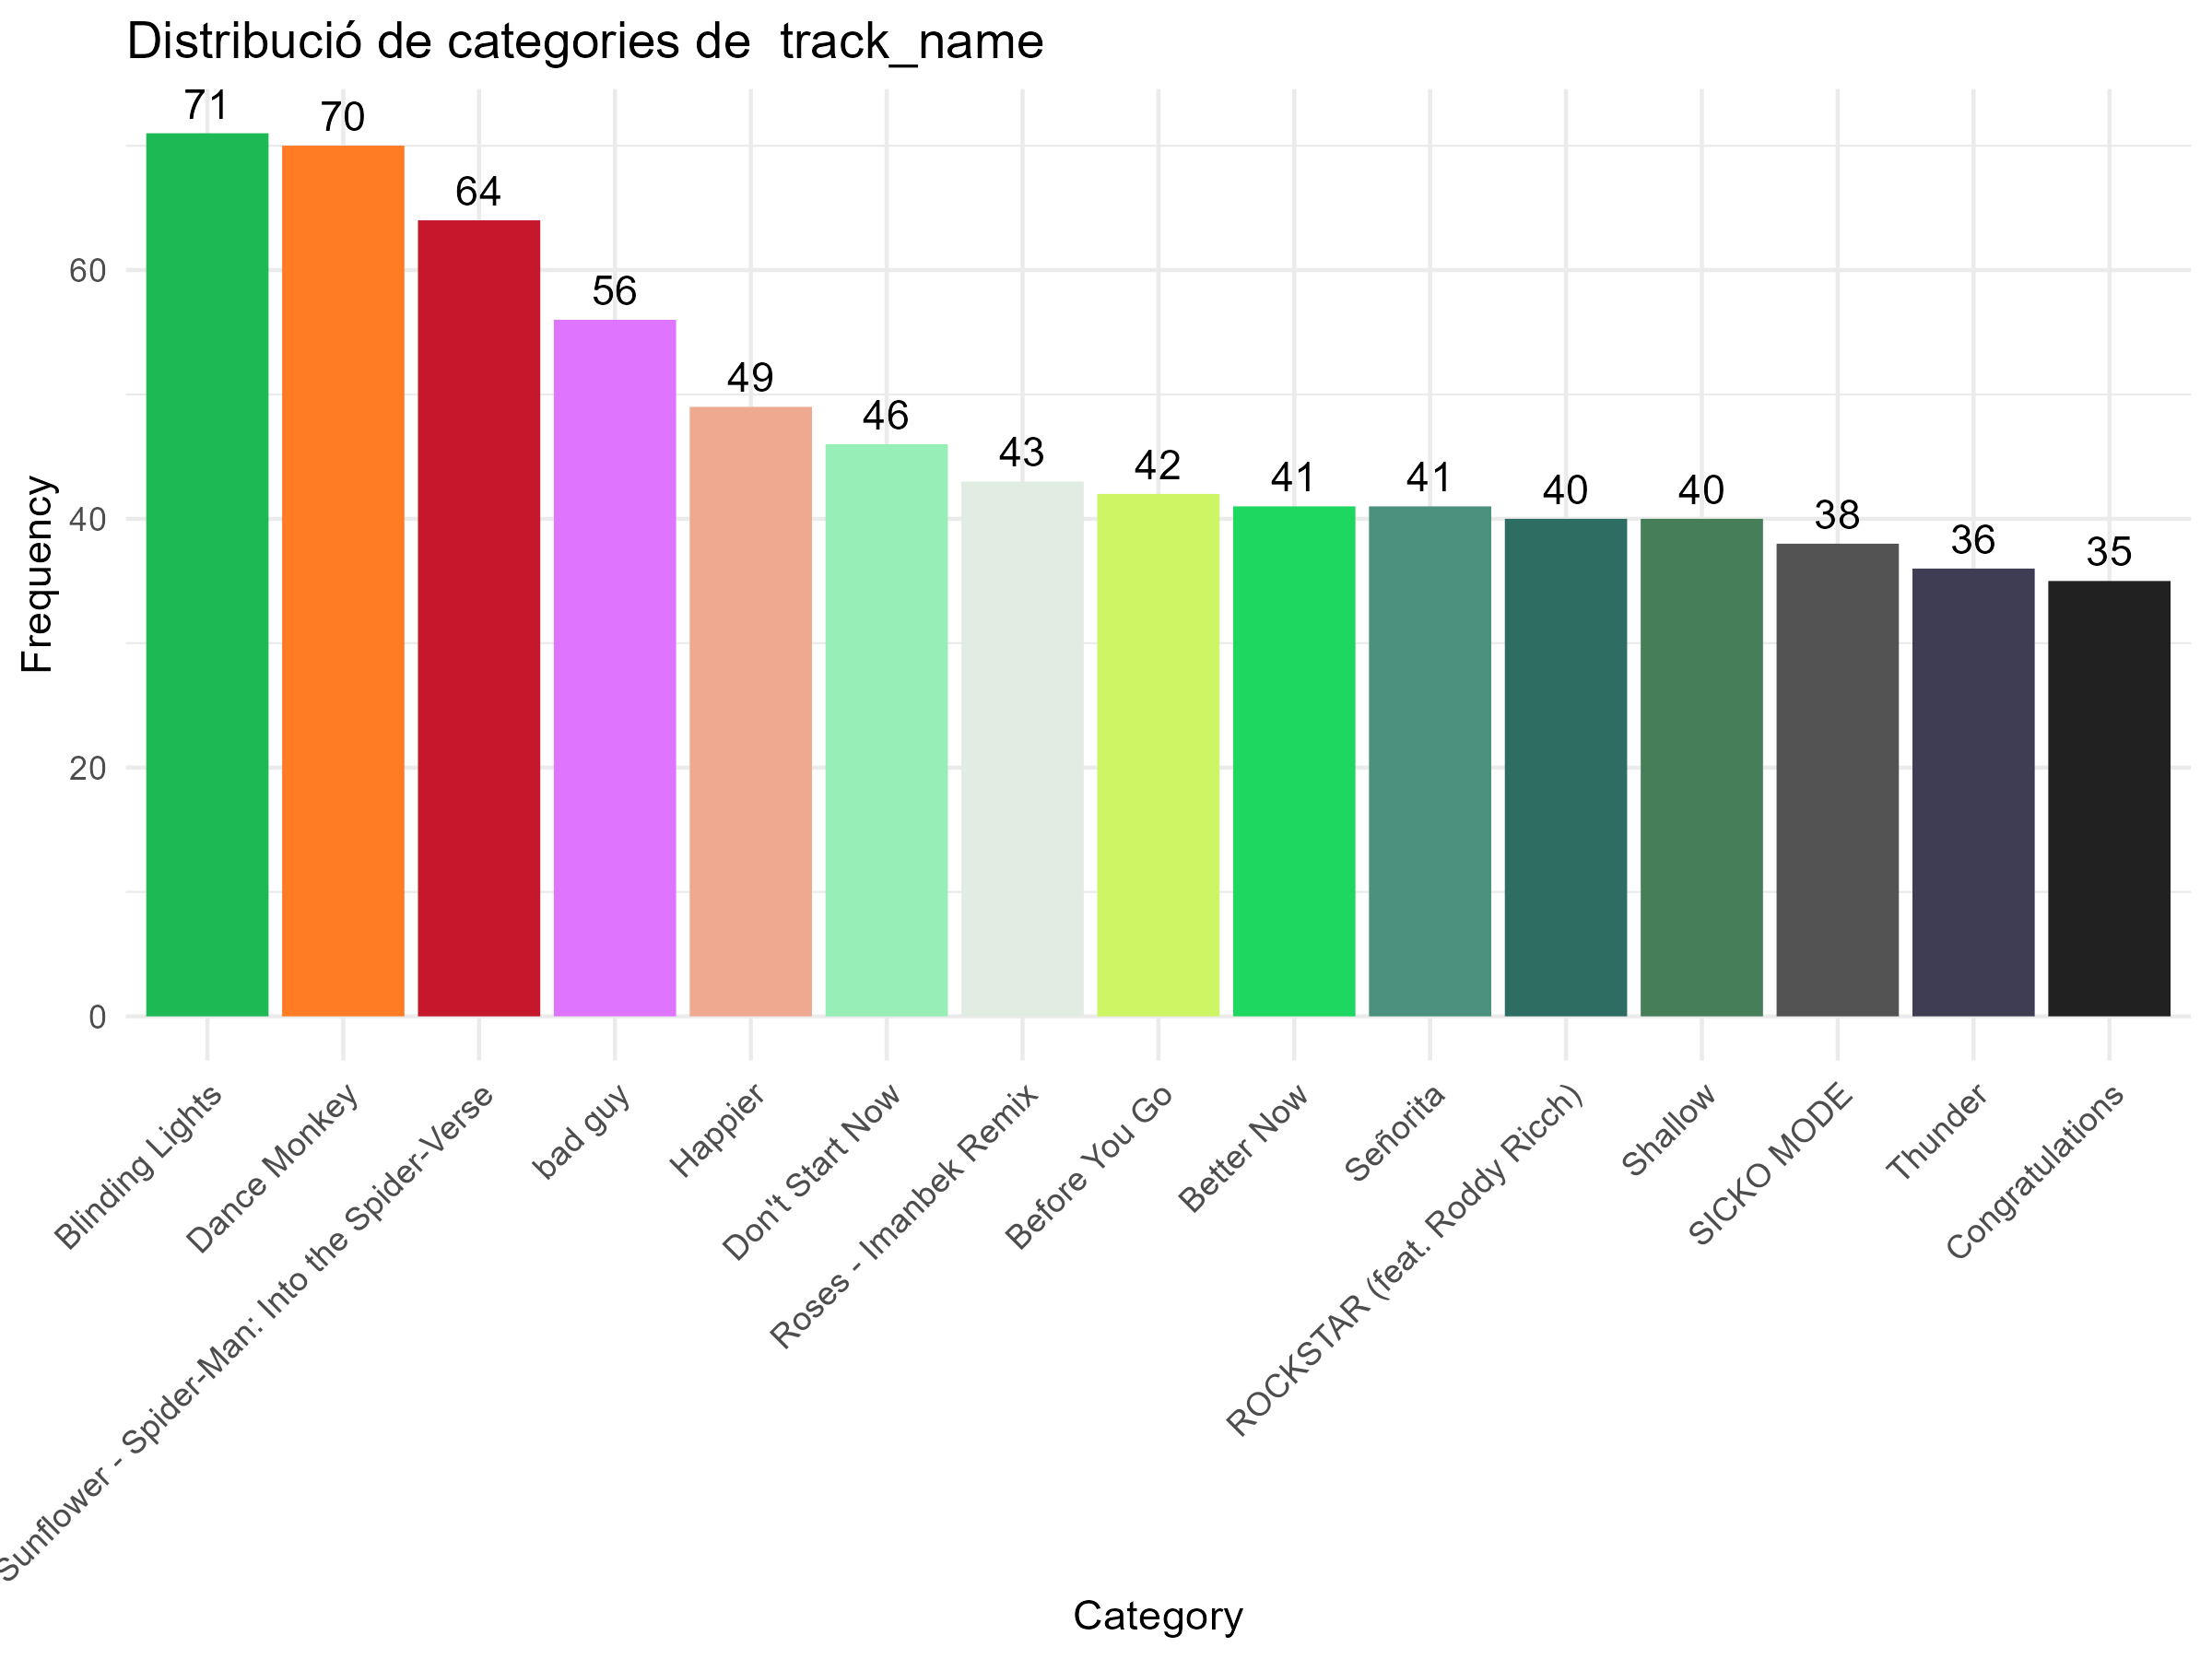
\includegraphics[width=0.95\linewidth]{Images/2_Univariate/bar_track_name.png}
        \caption{Bar plot de \textit{track\_name}}
        \label{fig:UnivariateR_track}
    \end{minipage}%
    \begin{minipage}{.4\textwidth}
        \centering
        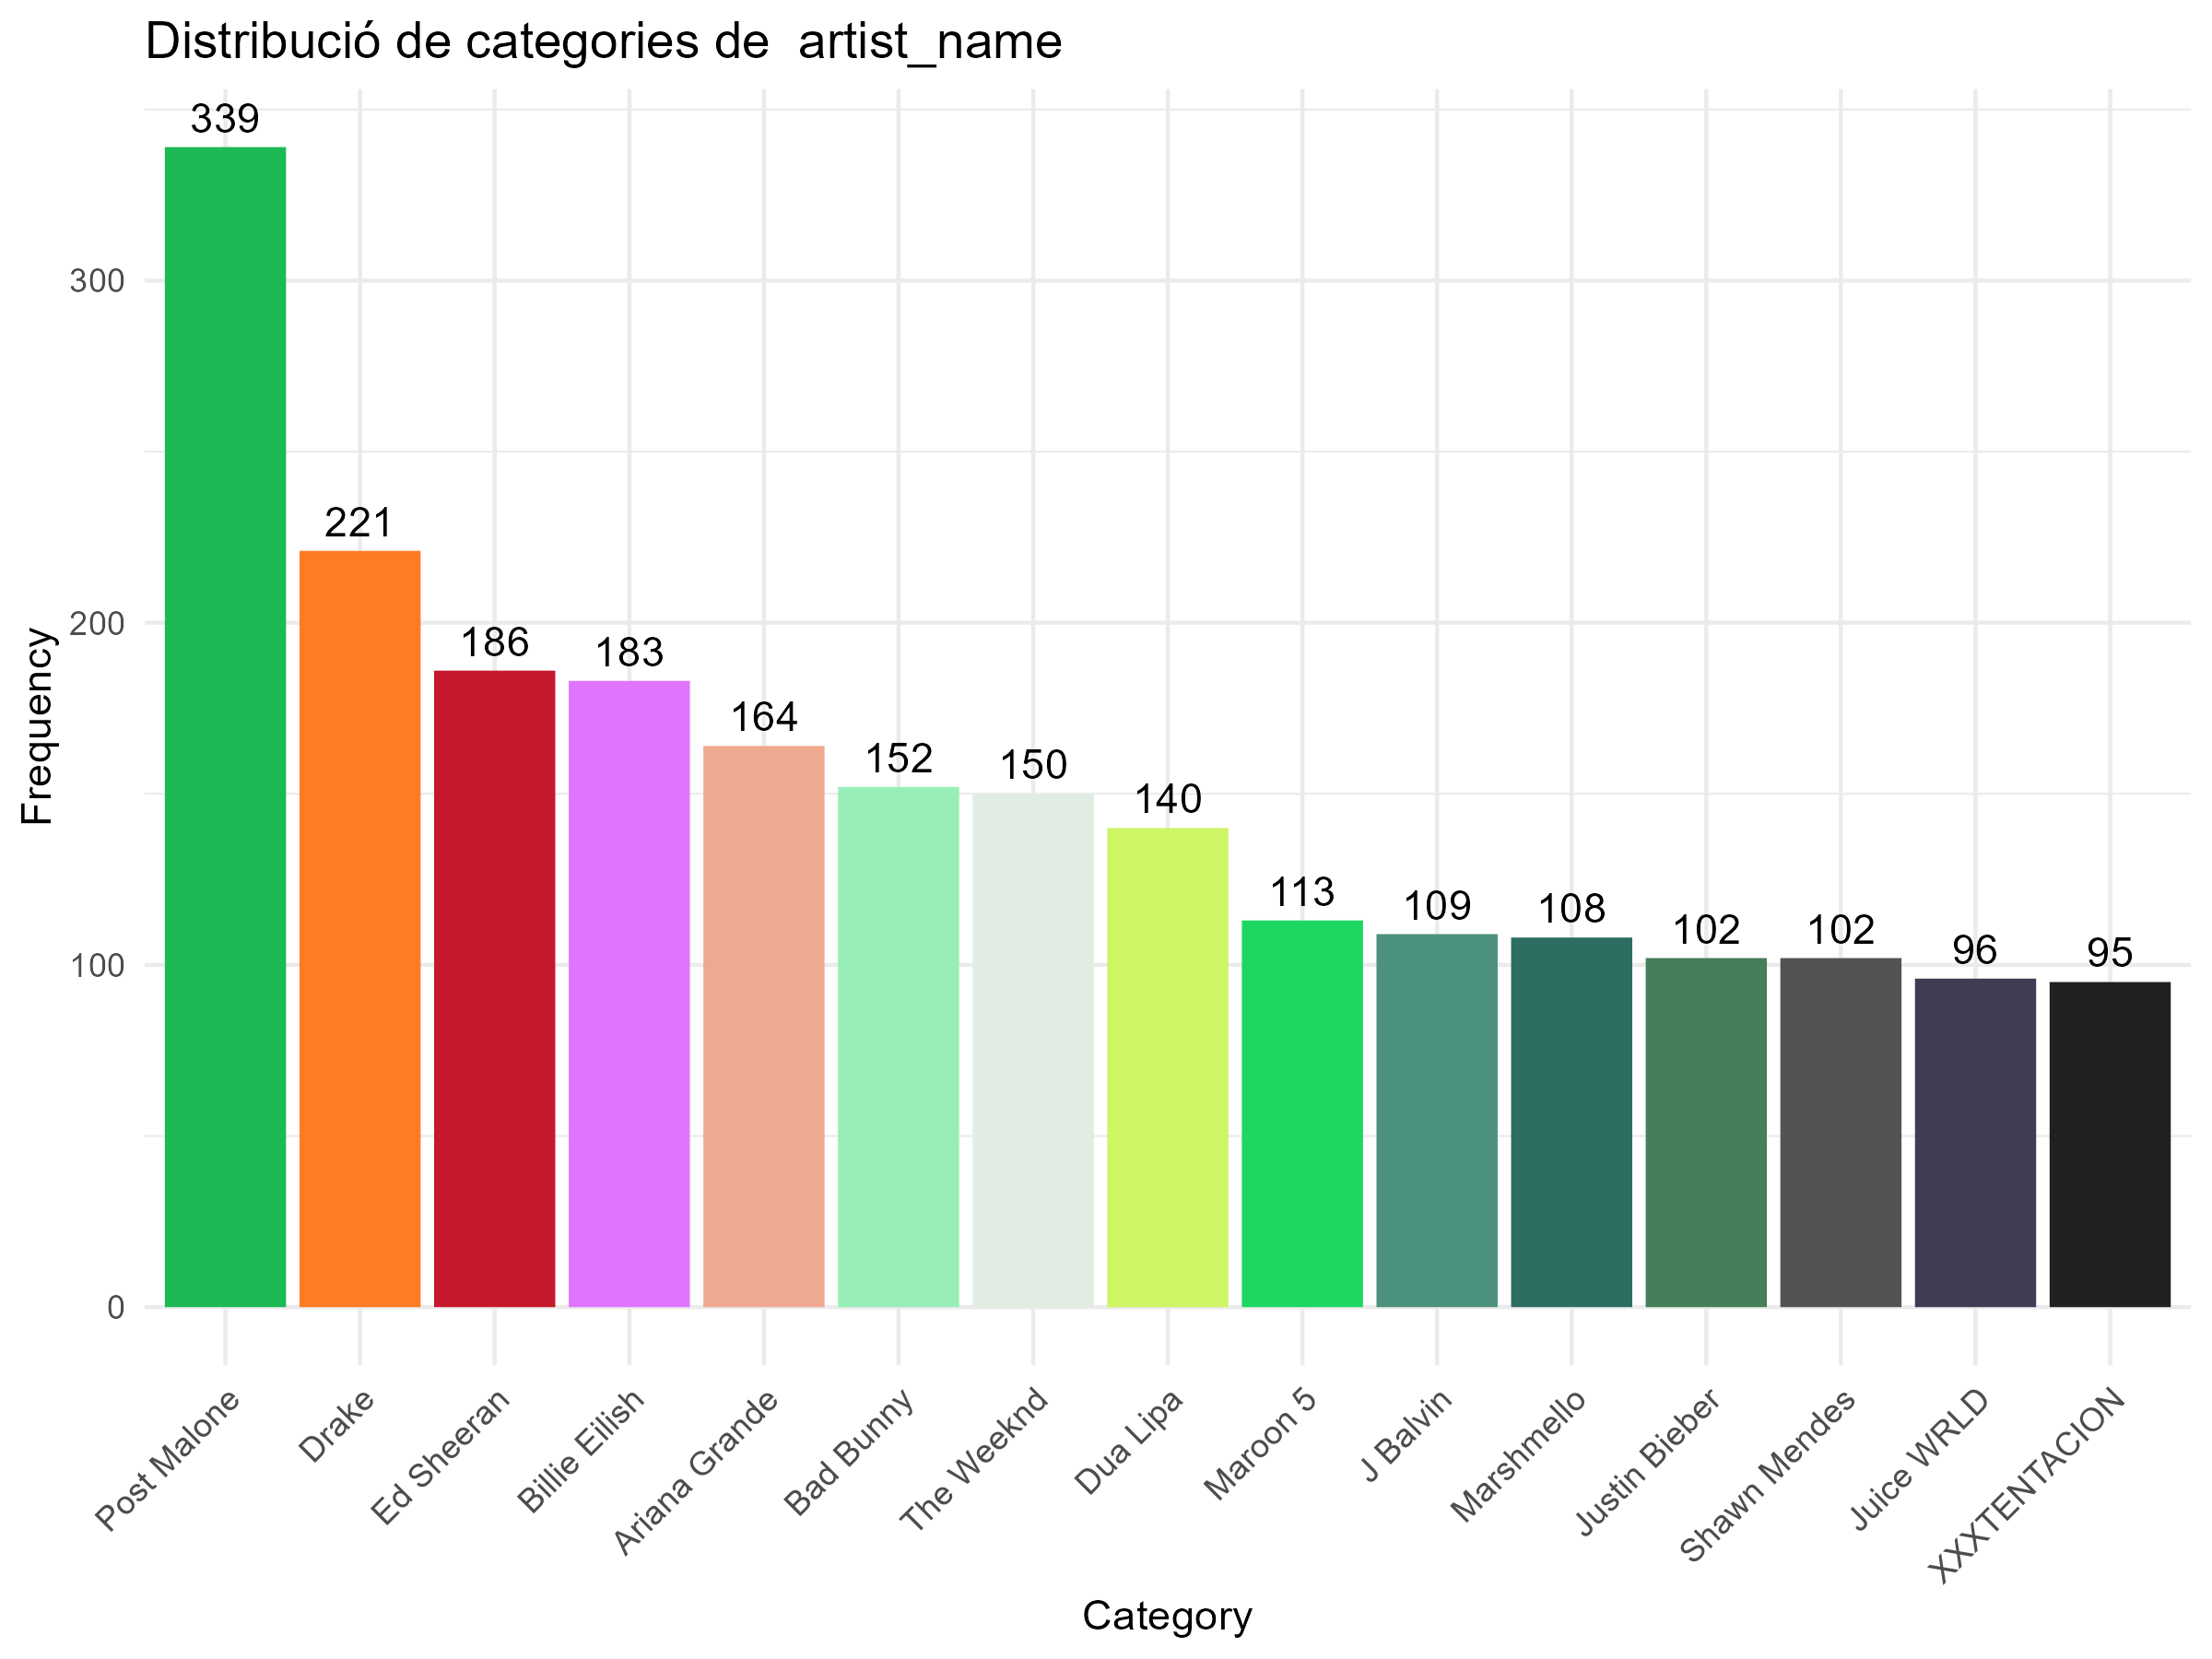
\includegraphics[width=0.95\linewidth]{Images/2_Univariate/bar_artist_name.png}
        \caption{Bar plot de \textit{artist\_name}}
        \label{fig:UnivariateR_artist}
    \end{minipage}%
\end{figure}

Pel que fa als gèneres de les cançons, el 69.6\% pertanyen al gènere pop (\ref{fig:UnivariateR_pop}). El 47.1\% són de hip-hop (\ref{fig:UnivariateR_hiphop}), i el 37.4\% electro (\ref{fig:UnivariateR_electro}) i un 12.3\% latino (\ref{fig:UnivariateR_latino}). La resta de gèneres (rock, christmas i cinema) tenen menys d'un 5\% d'aparicions.

\begin{figure}[H]
\centering
    \begin{minipage}{.4\textwidth}
        \centering
        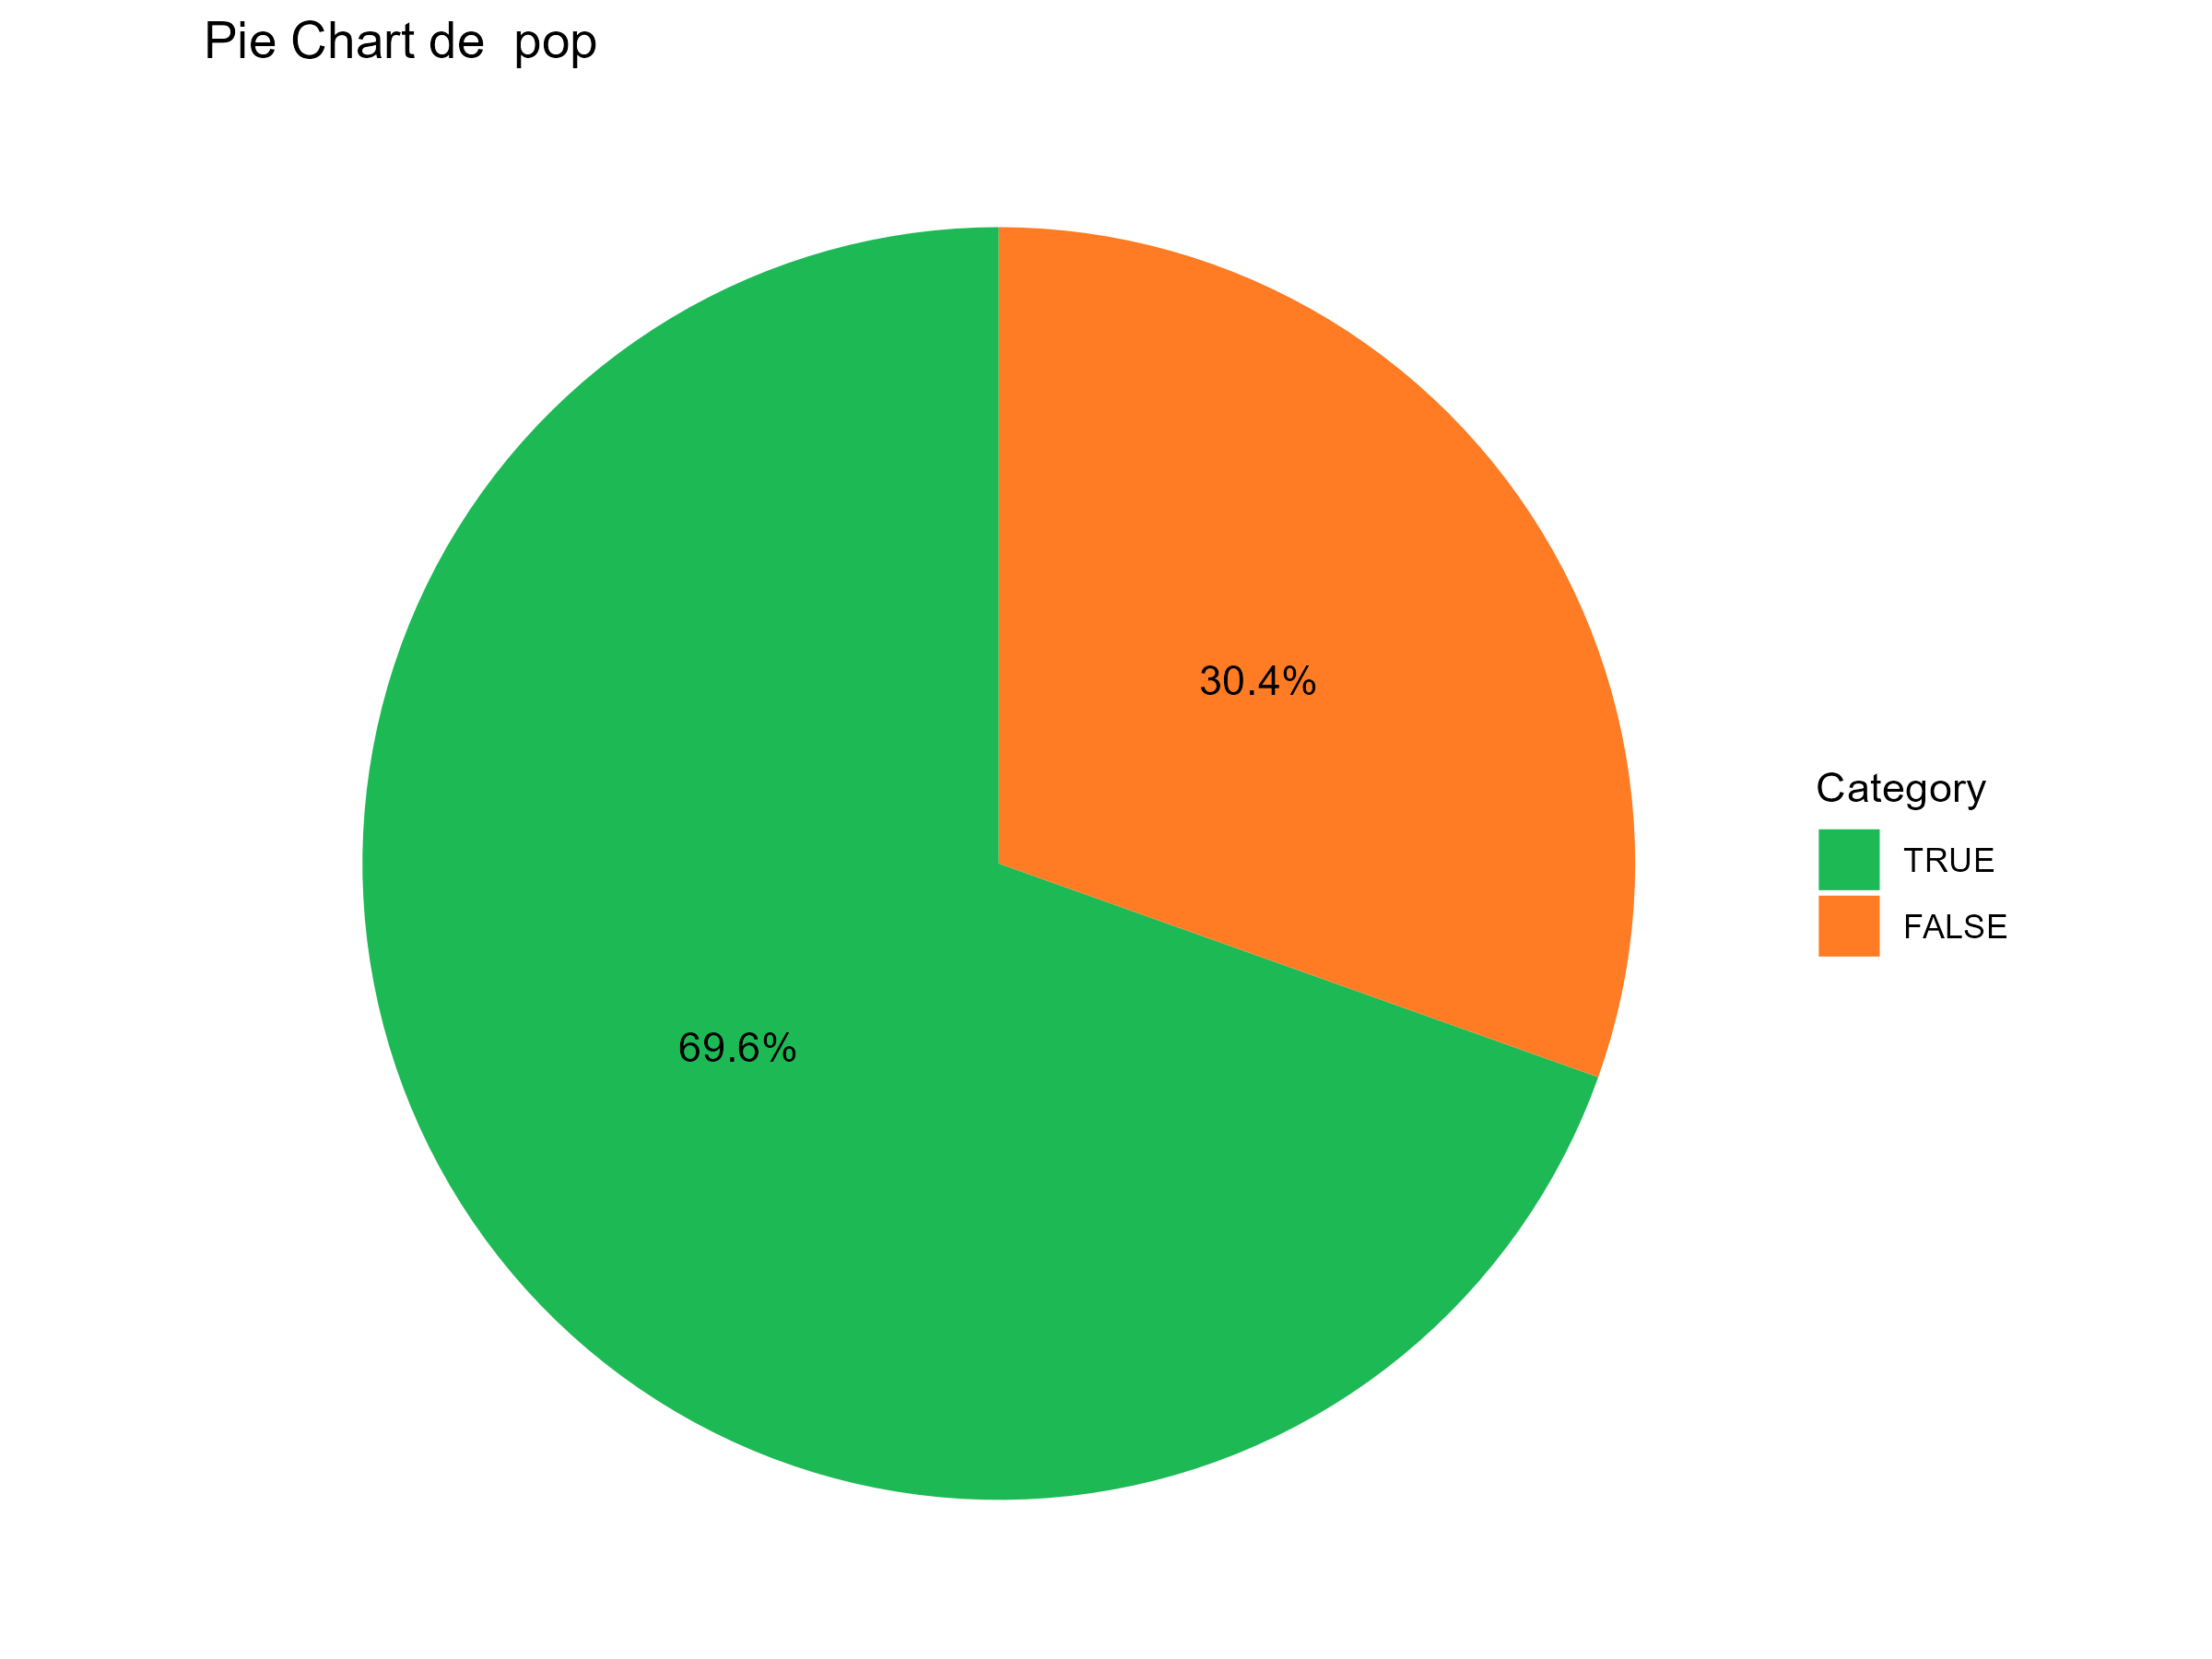
\includegraphics[width=0.95\linewidth]{Images/2_Univariate/pie_pop.png}
        \caption{Pie plot de \textit{pop}}
        \label{fig:UnivariateR_pop}
    \end{minipage}%
    \begin{minipage}{.4\textwidth}
        \centering
        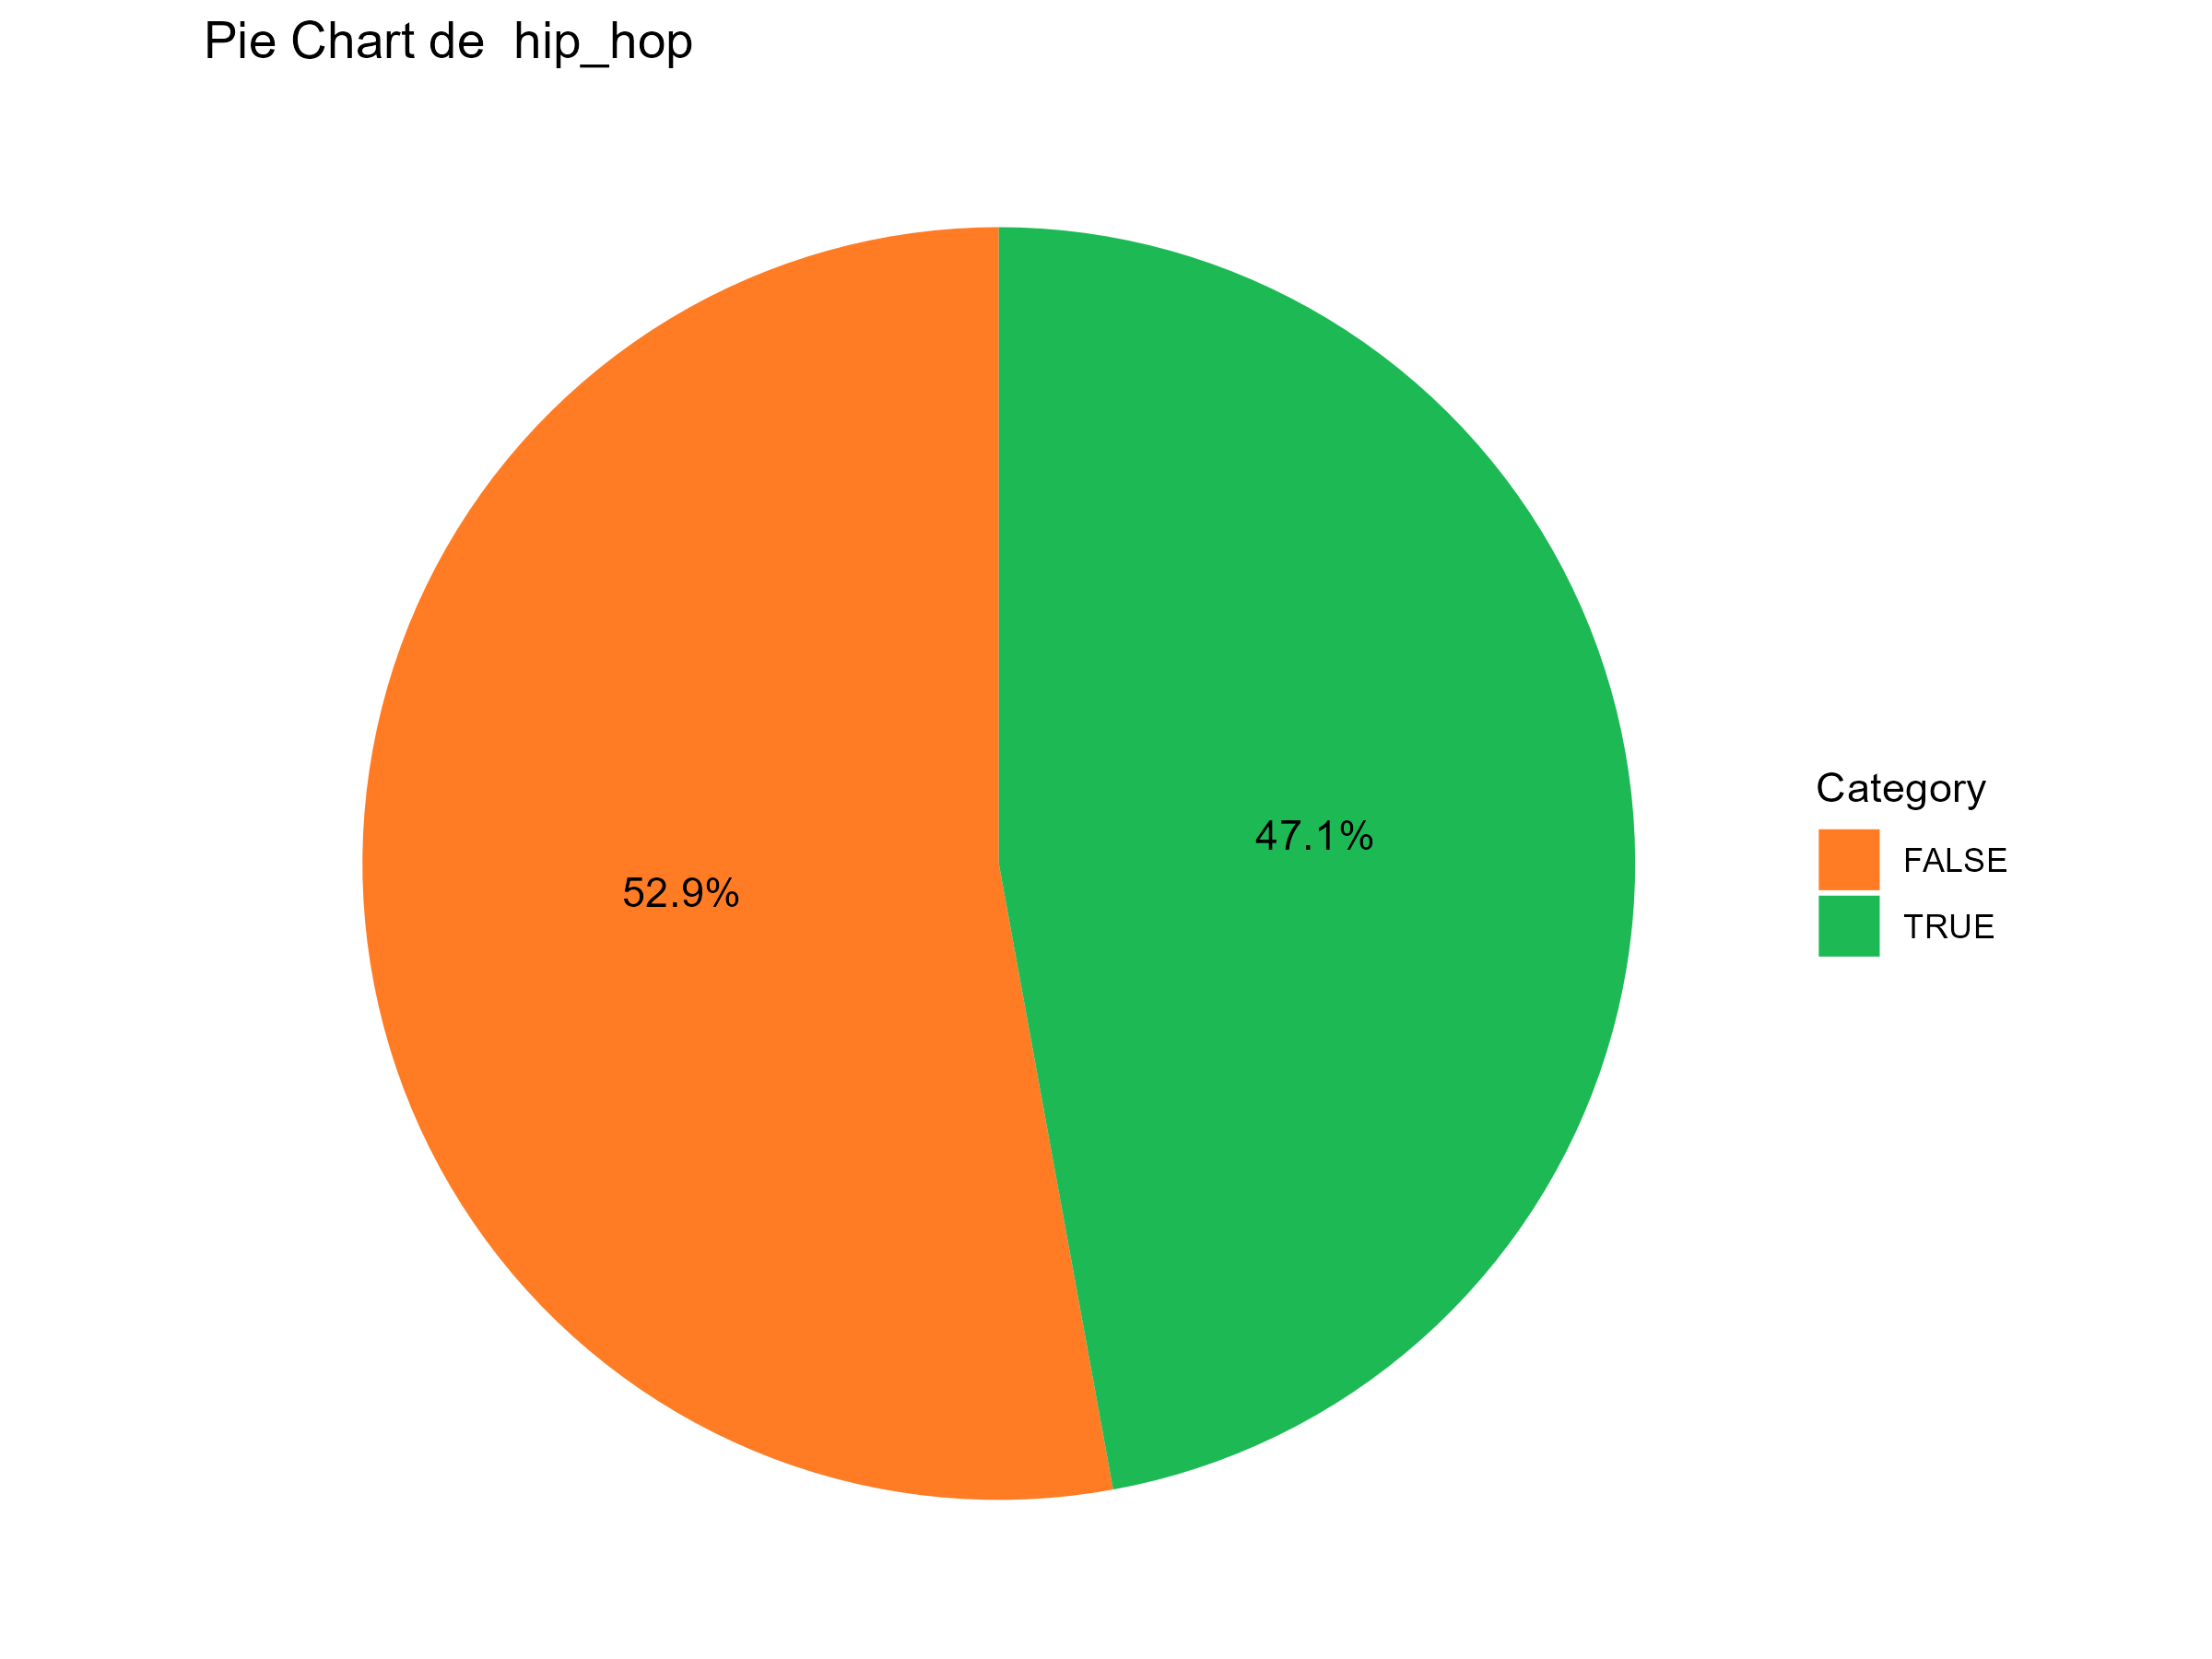
\includegraphics[width=0.95\linewidth]{Images/2_Univariate/pie_hip_hop.png}
        \caption{Bar plot de \textit{hip\_hop}}
        \label{fig:UnivariateR_hiphop}
    \end{minipage}%
\end{figure}

\begin{figure}[H]
\centering
    \begin{minipage}{.4\textwidth}
        \centering
        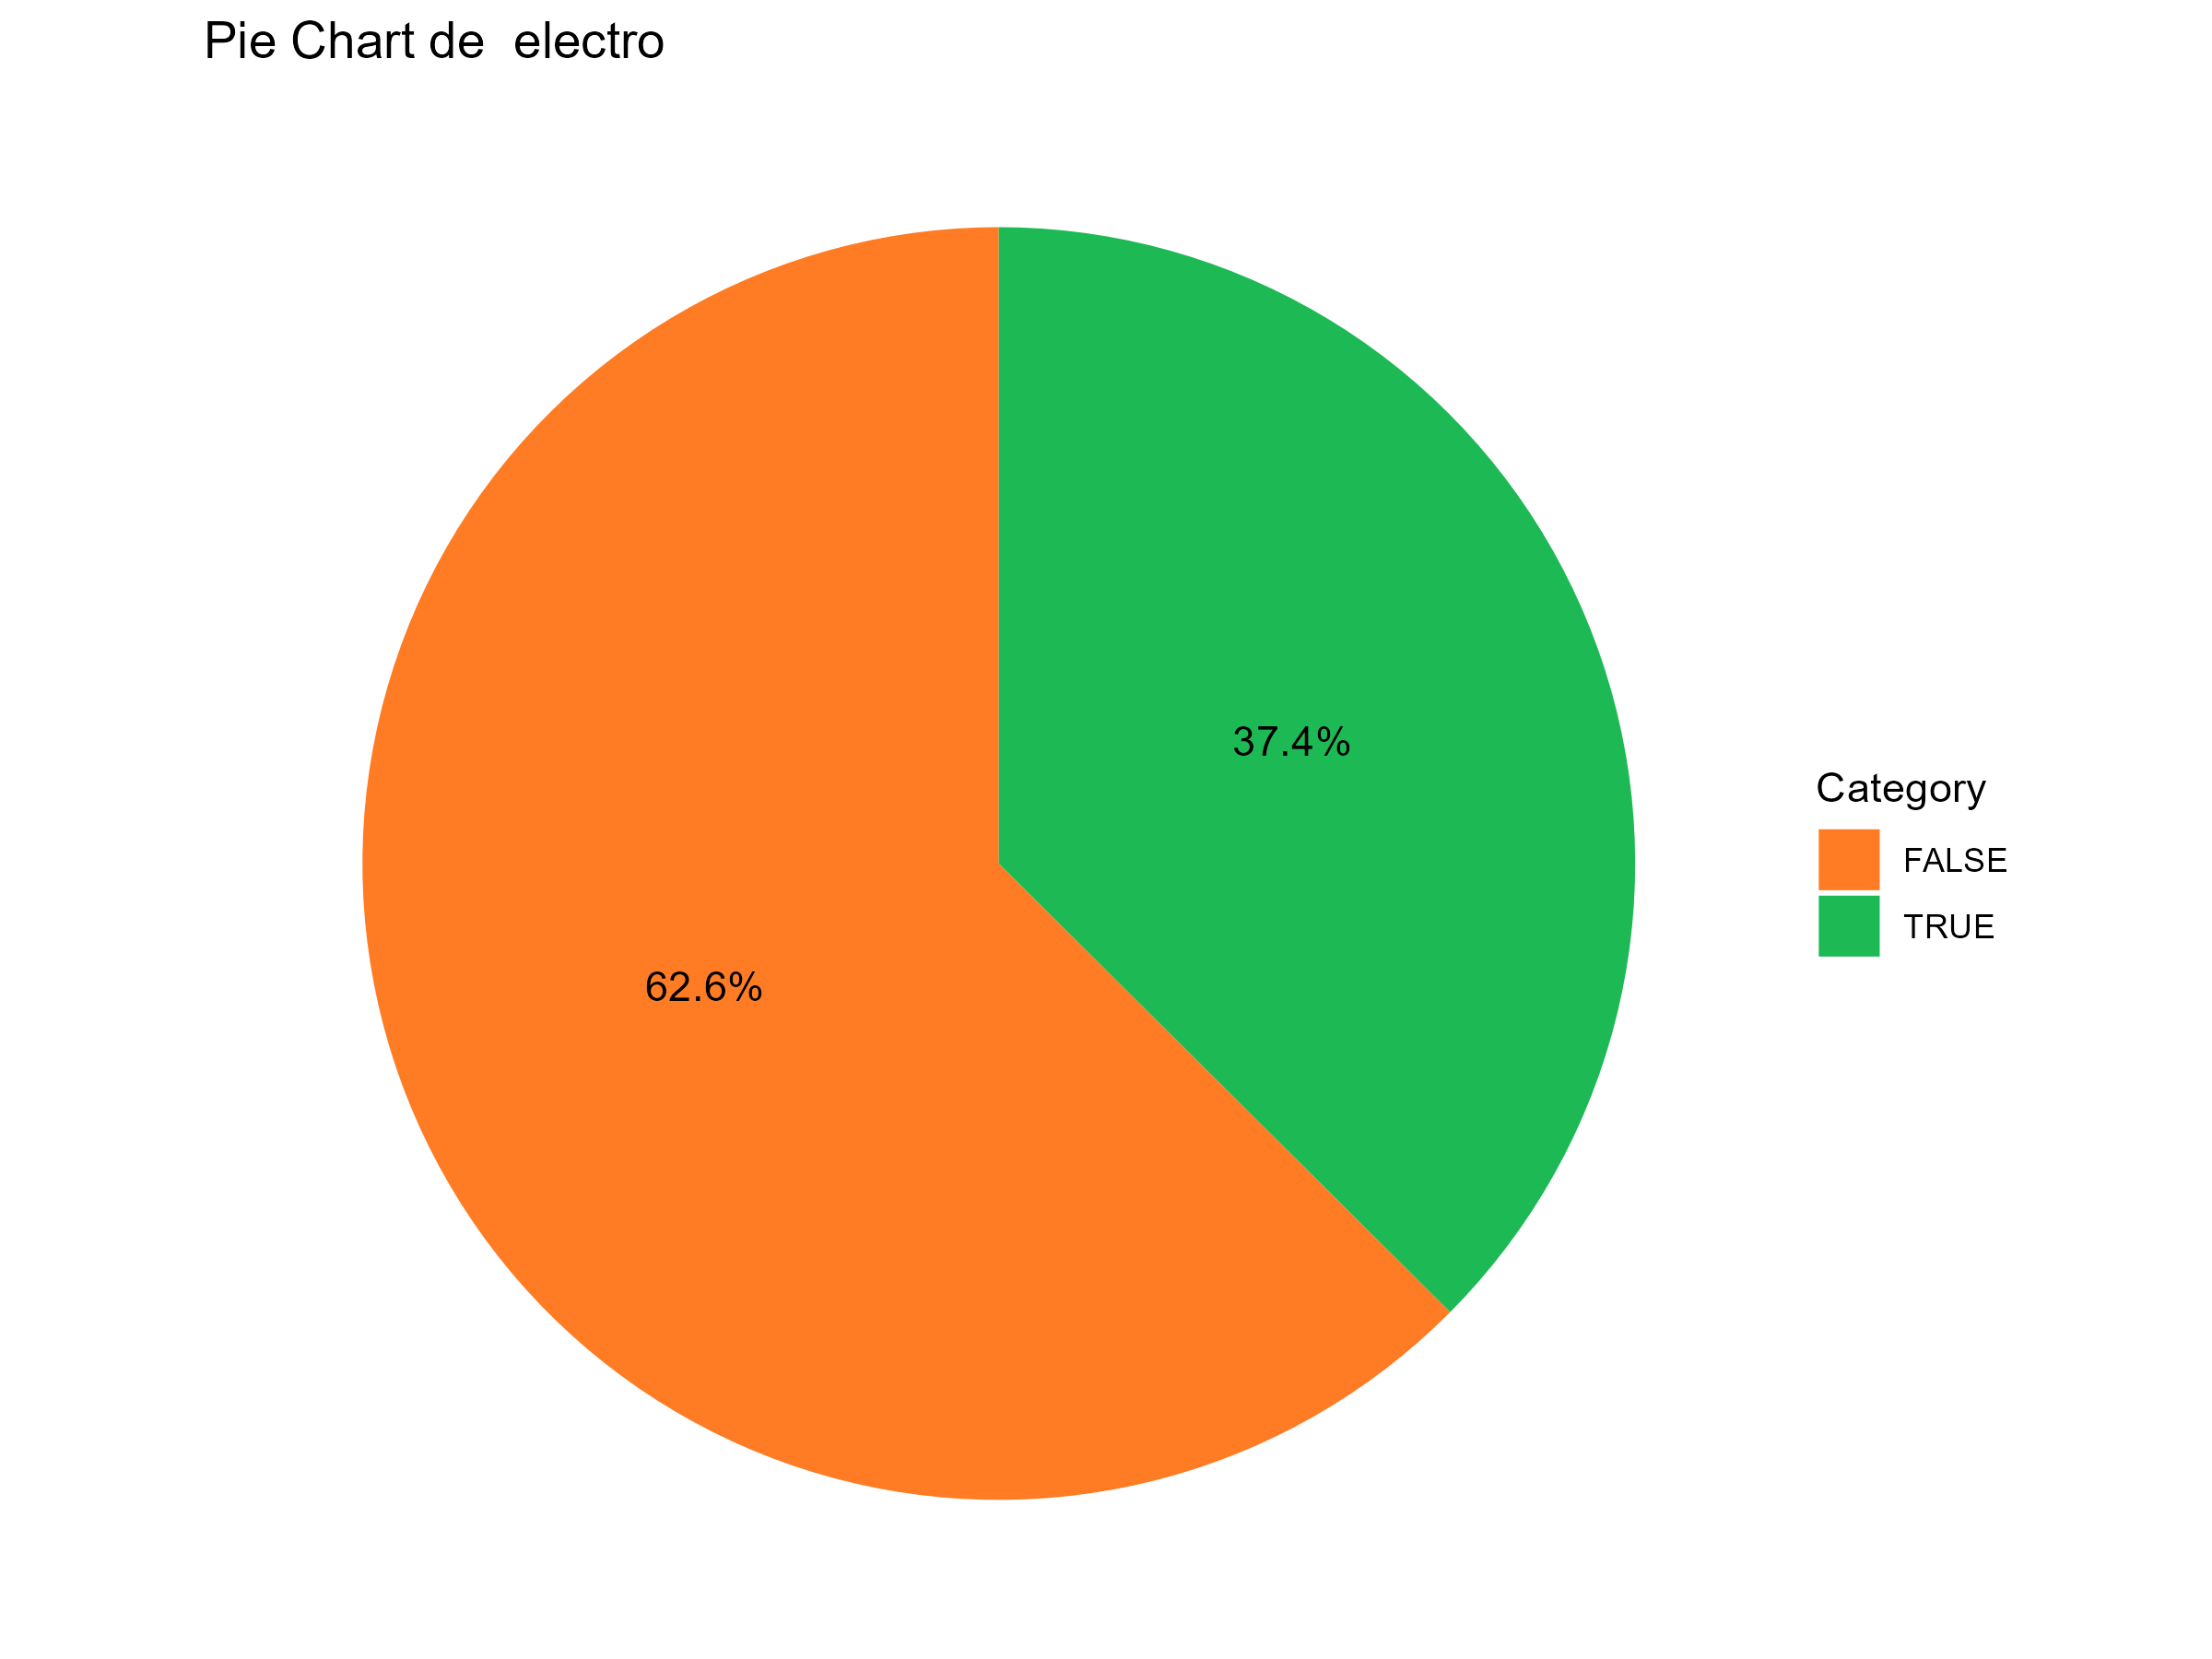
\includegraphics[width=0.95\linewidth]{Images/2_Univariate/pie_electro.png}
        \caption{Pie plot de \textit{electro}}
        \label{fig:UnivariateR_electro}
    \end{minipage}%
    \begin{minipage}{.4\textwidth}
        \centering
        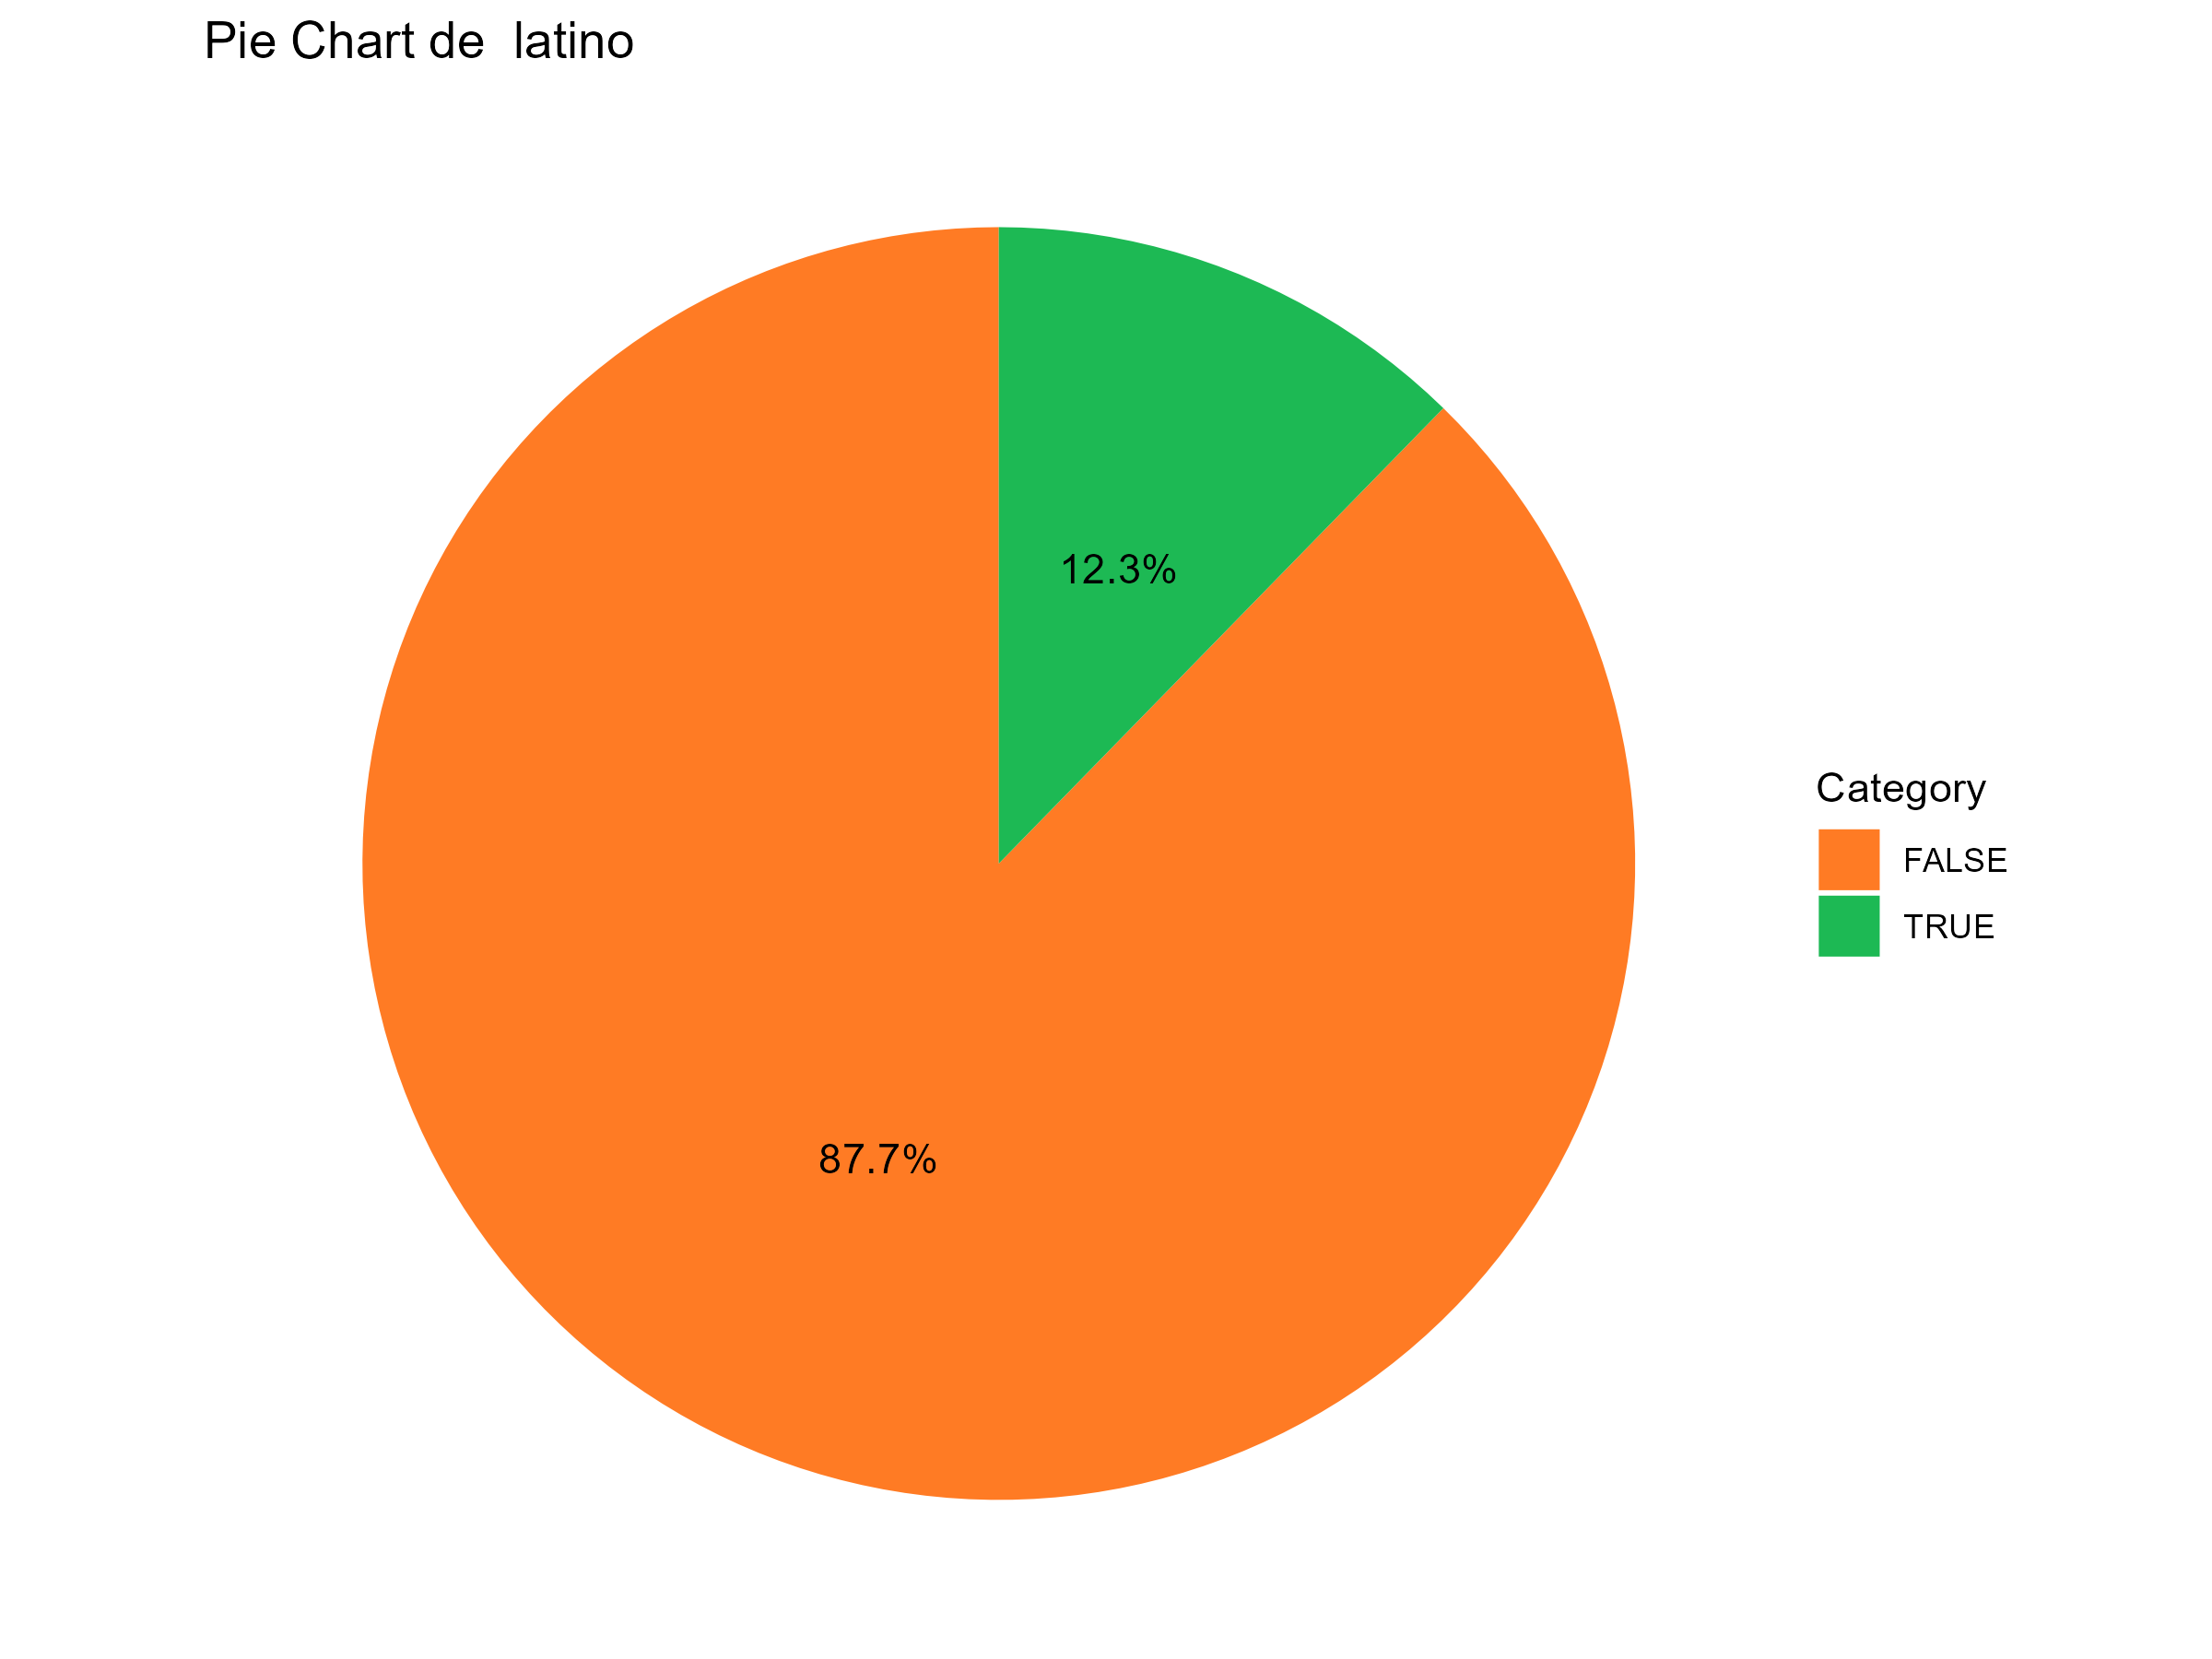
\includegraphics[width=0.95\linewidth]{Images/2_Univariate/pie_latino.png}
        \caption{Bar plot de \textit{latino}}
        \label{fig:UnivariateR_latino}
    \end{minipage}%
\end{figure}

Danceability i energy presenten unes distribucions bastant normals (figures \ref{fig:UnivariateR_danceability} i \ref{fig:UnivariateR_energy}), lleugerament desviades cap a valors majors a 0.5. En canvi, liveness o acousticness presenten distribucions més aviat exponencials (figures \ref{fig:UnivariateR_liveness} i \ref{fig:UnivariateR_acousticness}).

\begin{figure}[H]
\centering
    \begin{minipage}{.4\textwidth}
        \centering
        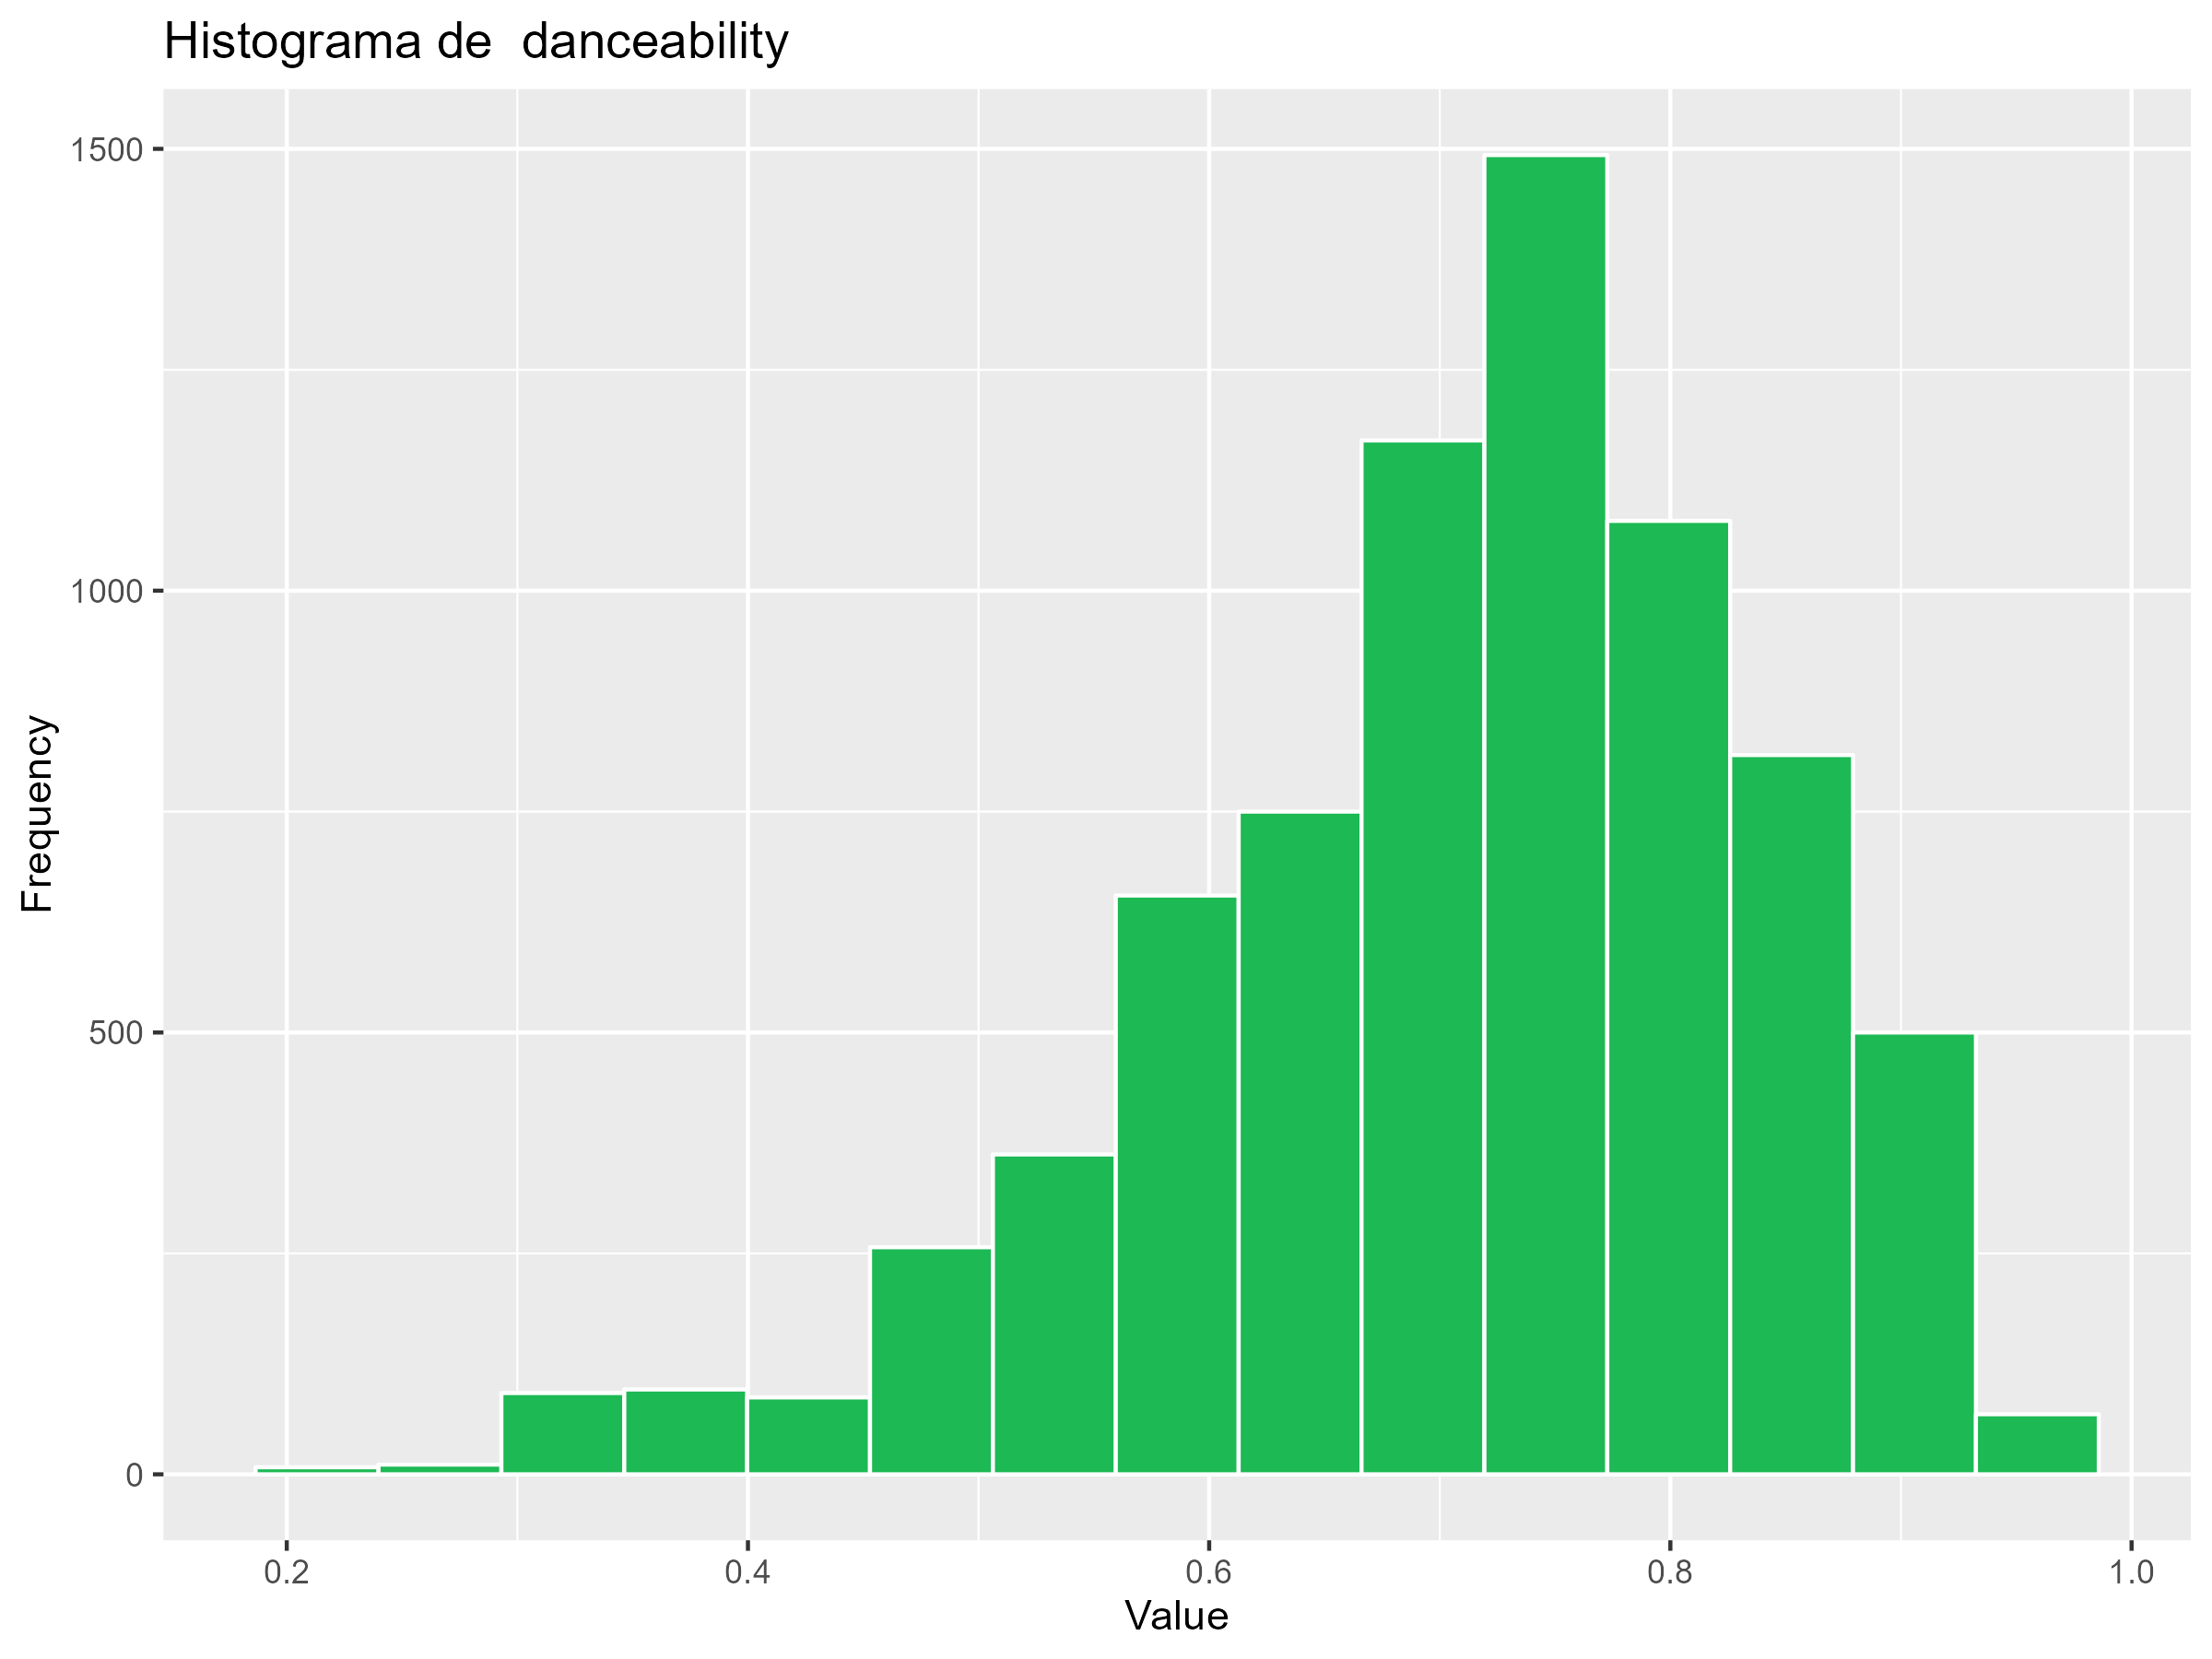
\includegraphics[width=0.95\linewidth]{Images/2_Univariate/hist_danceability.png}
        \caption{Histograma de \textit{danceability}}
        \label{fig:UnivariateR_danceability}
    \end{minipage}%
    \begin{minipage}{.4\textwidth}
        \centering
        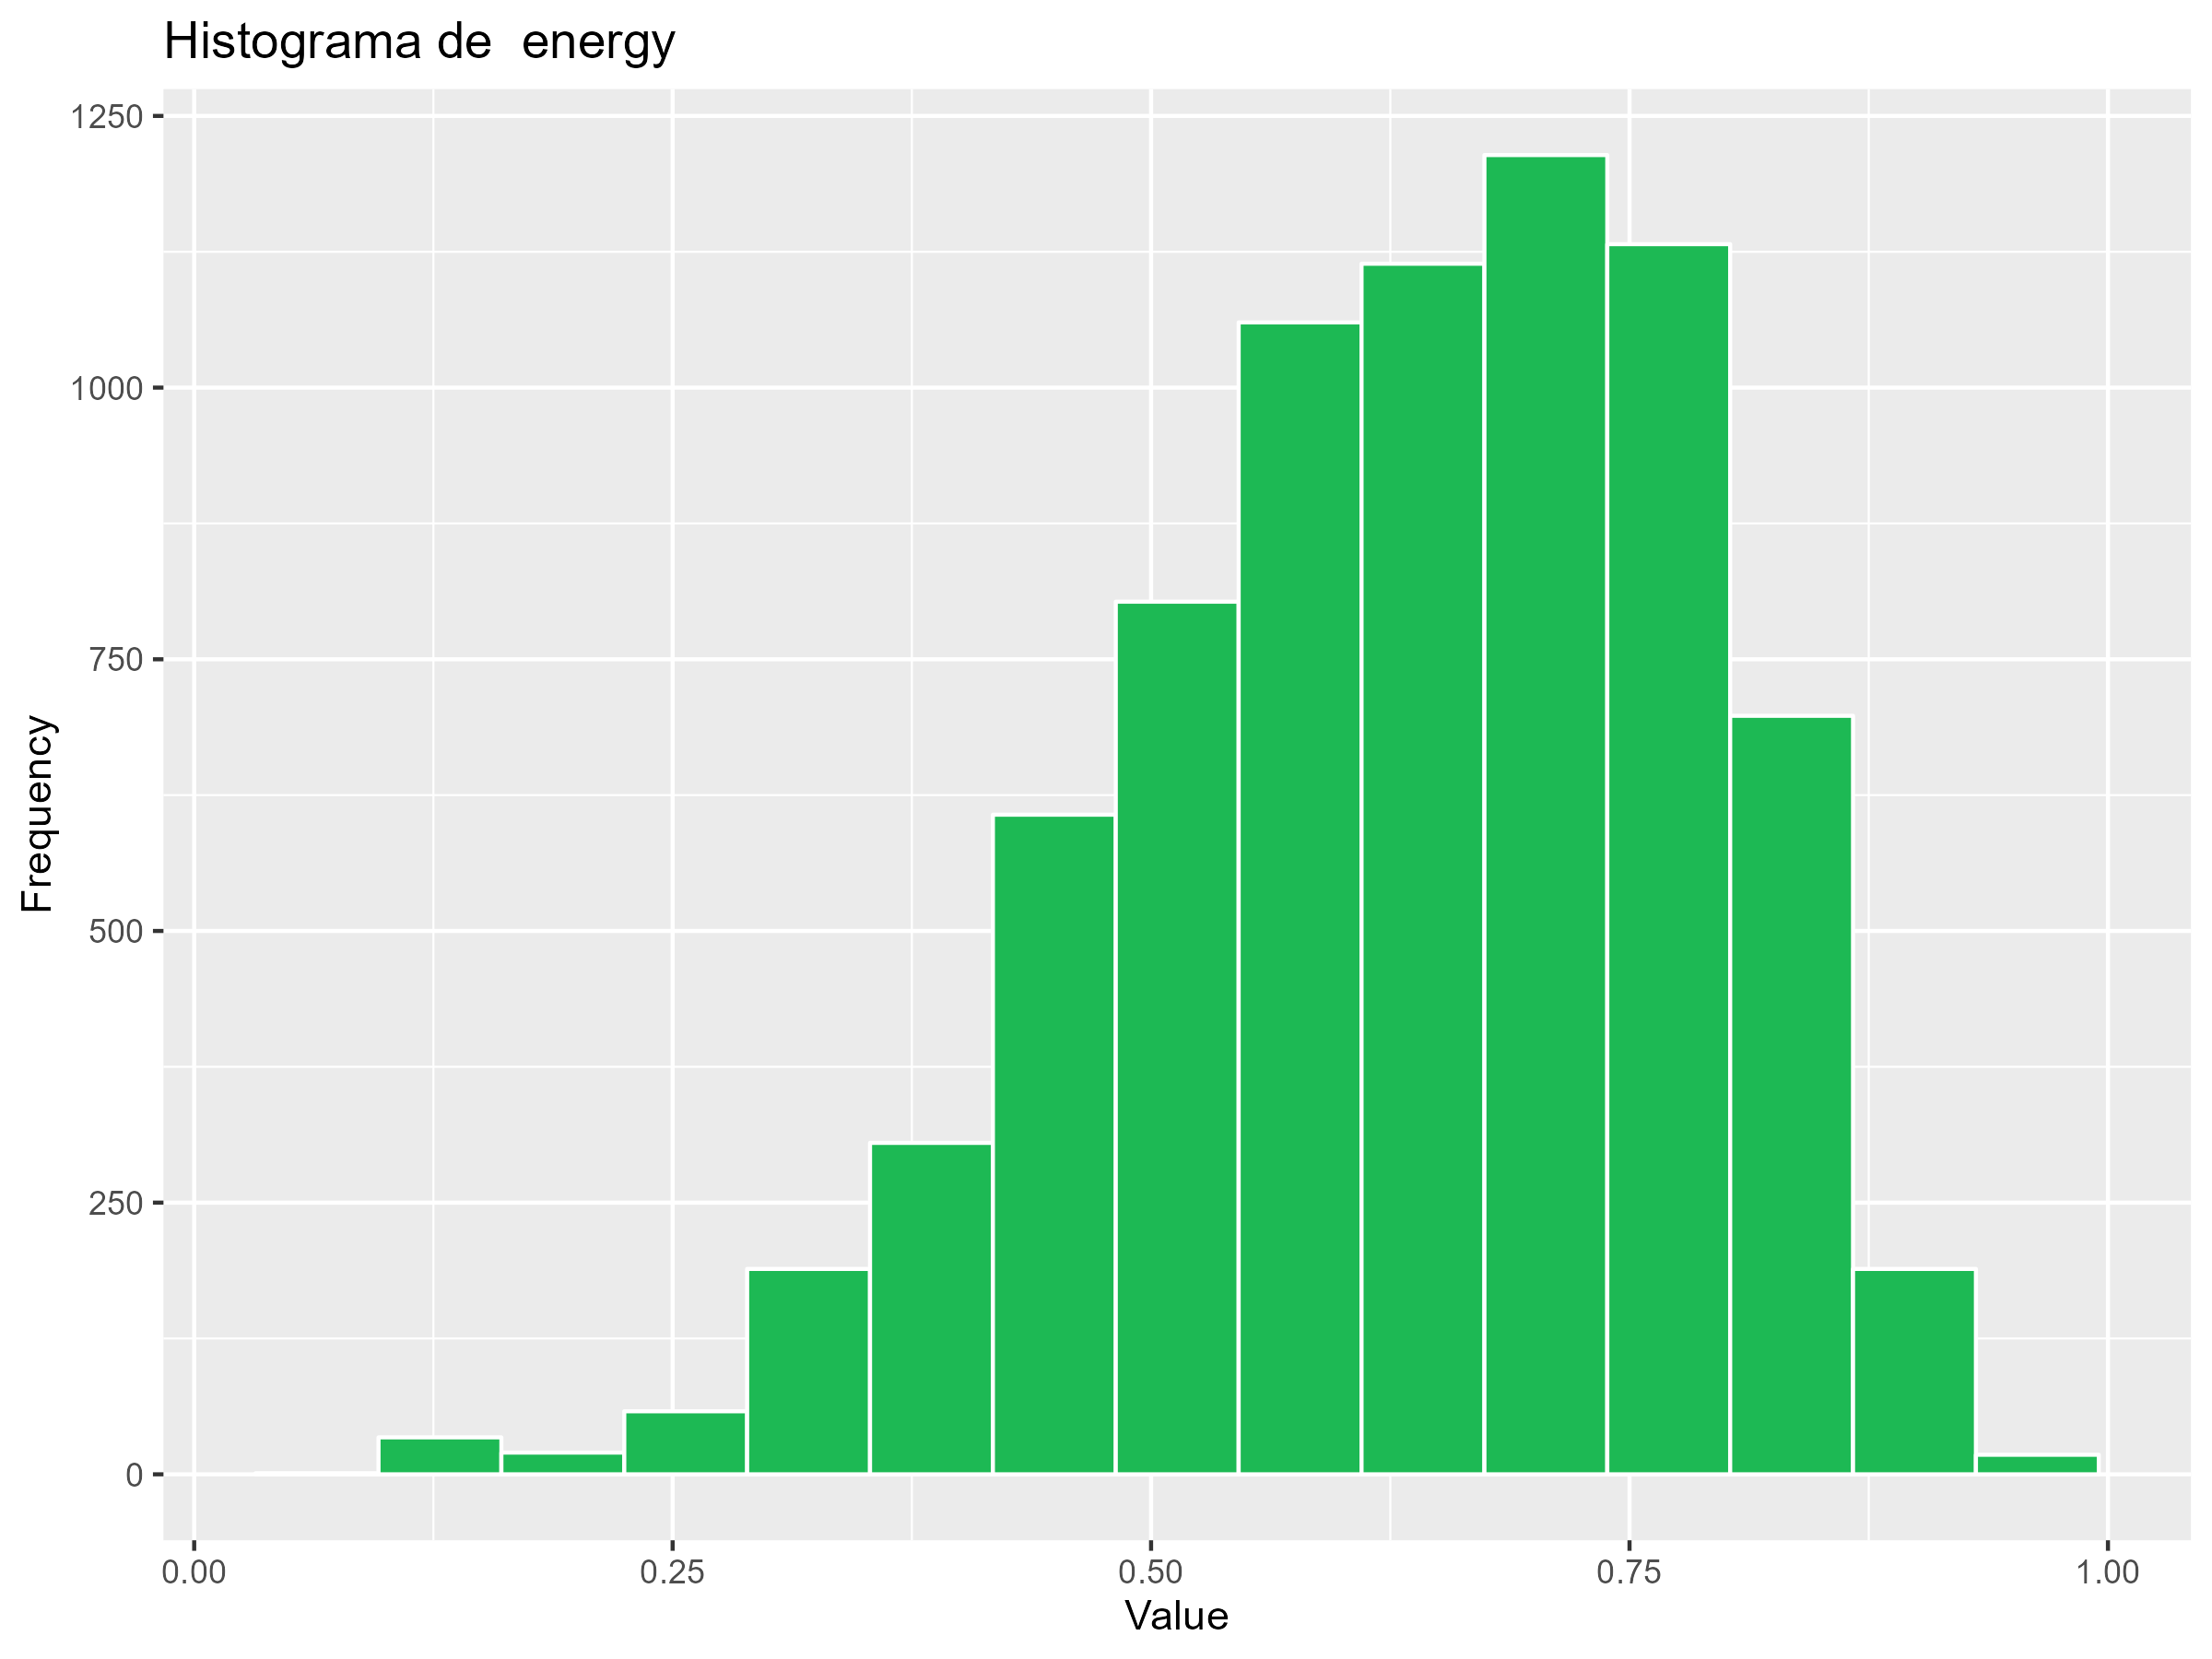
\includegraphics[width=0.95\linewidth]{Images/2_Univariate/hist_energy.png}
        \caption{Histograma de \textit{energy}}
        \label{fig:UnivariateR_energy}
    \end{minipage}%
\end{figure}

\begin{figure}[H]
\centering
    \begin{minipage}{.4\textwidth}
        \centering
        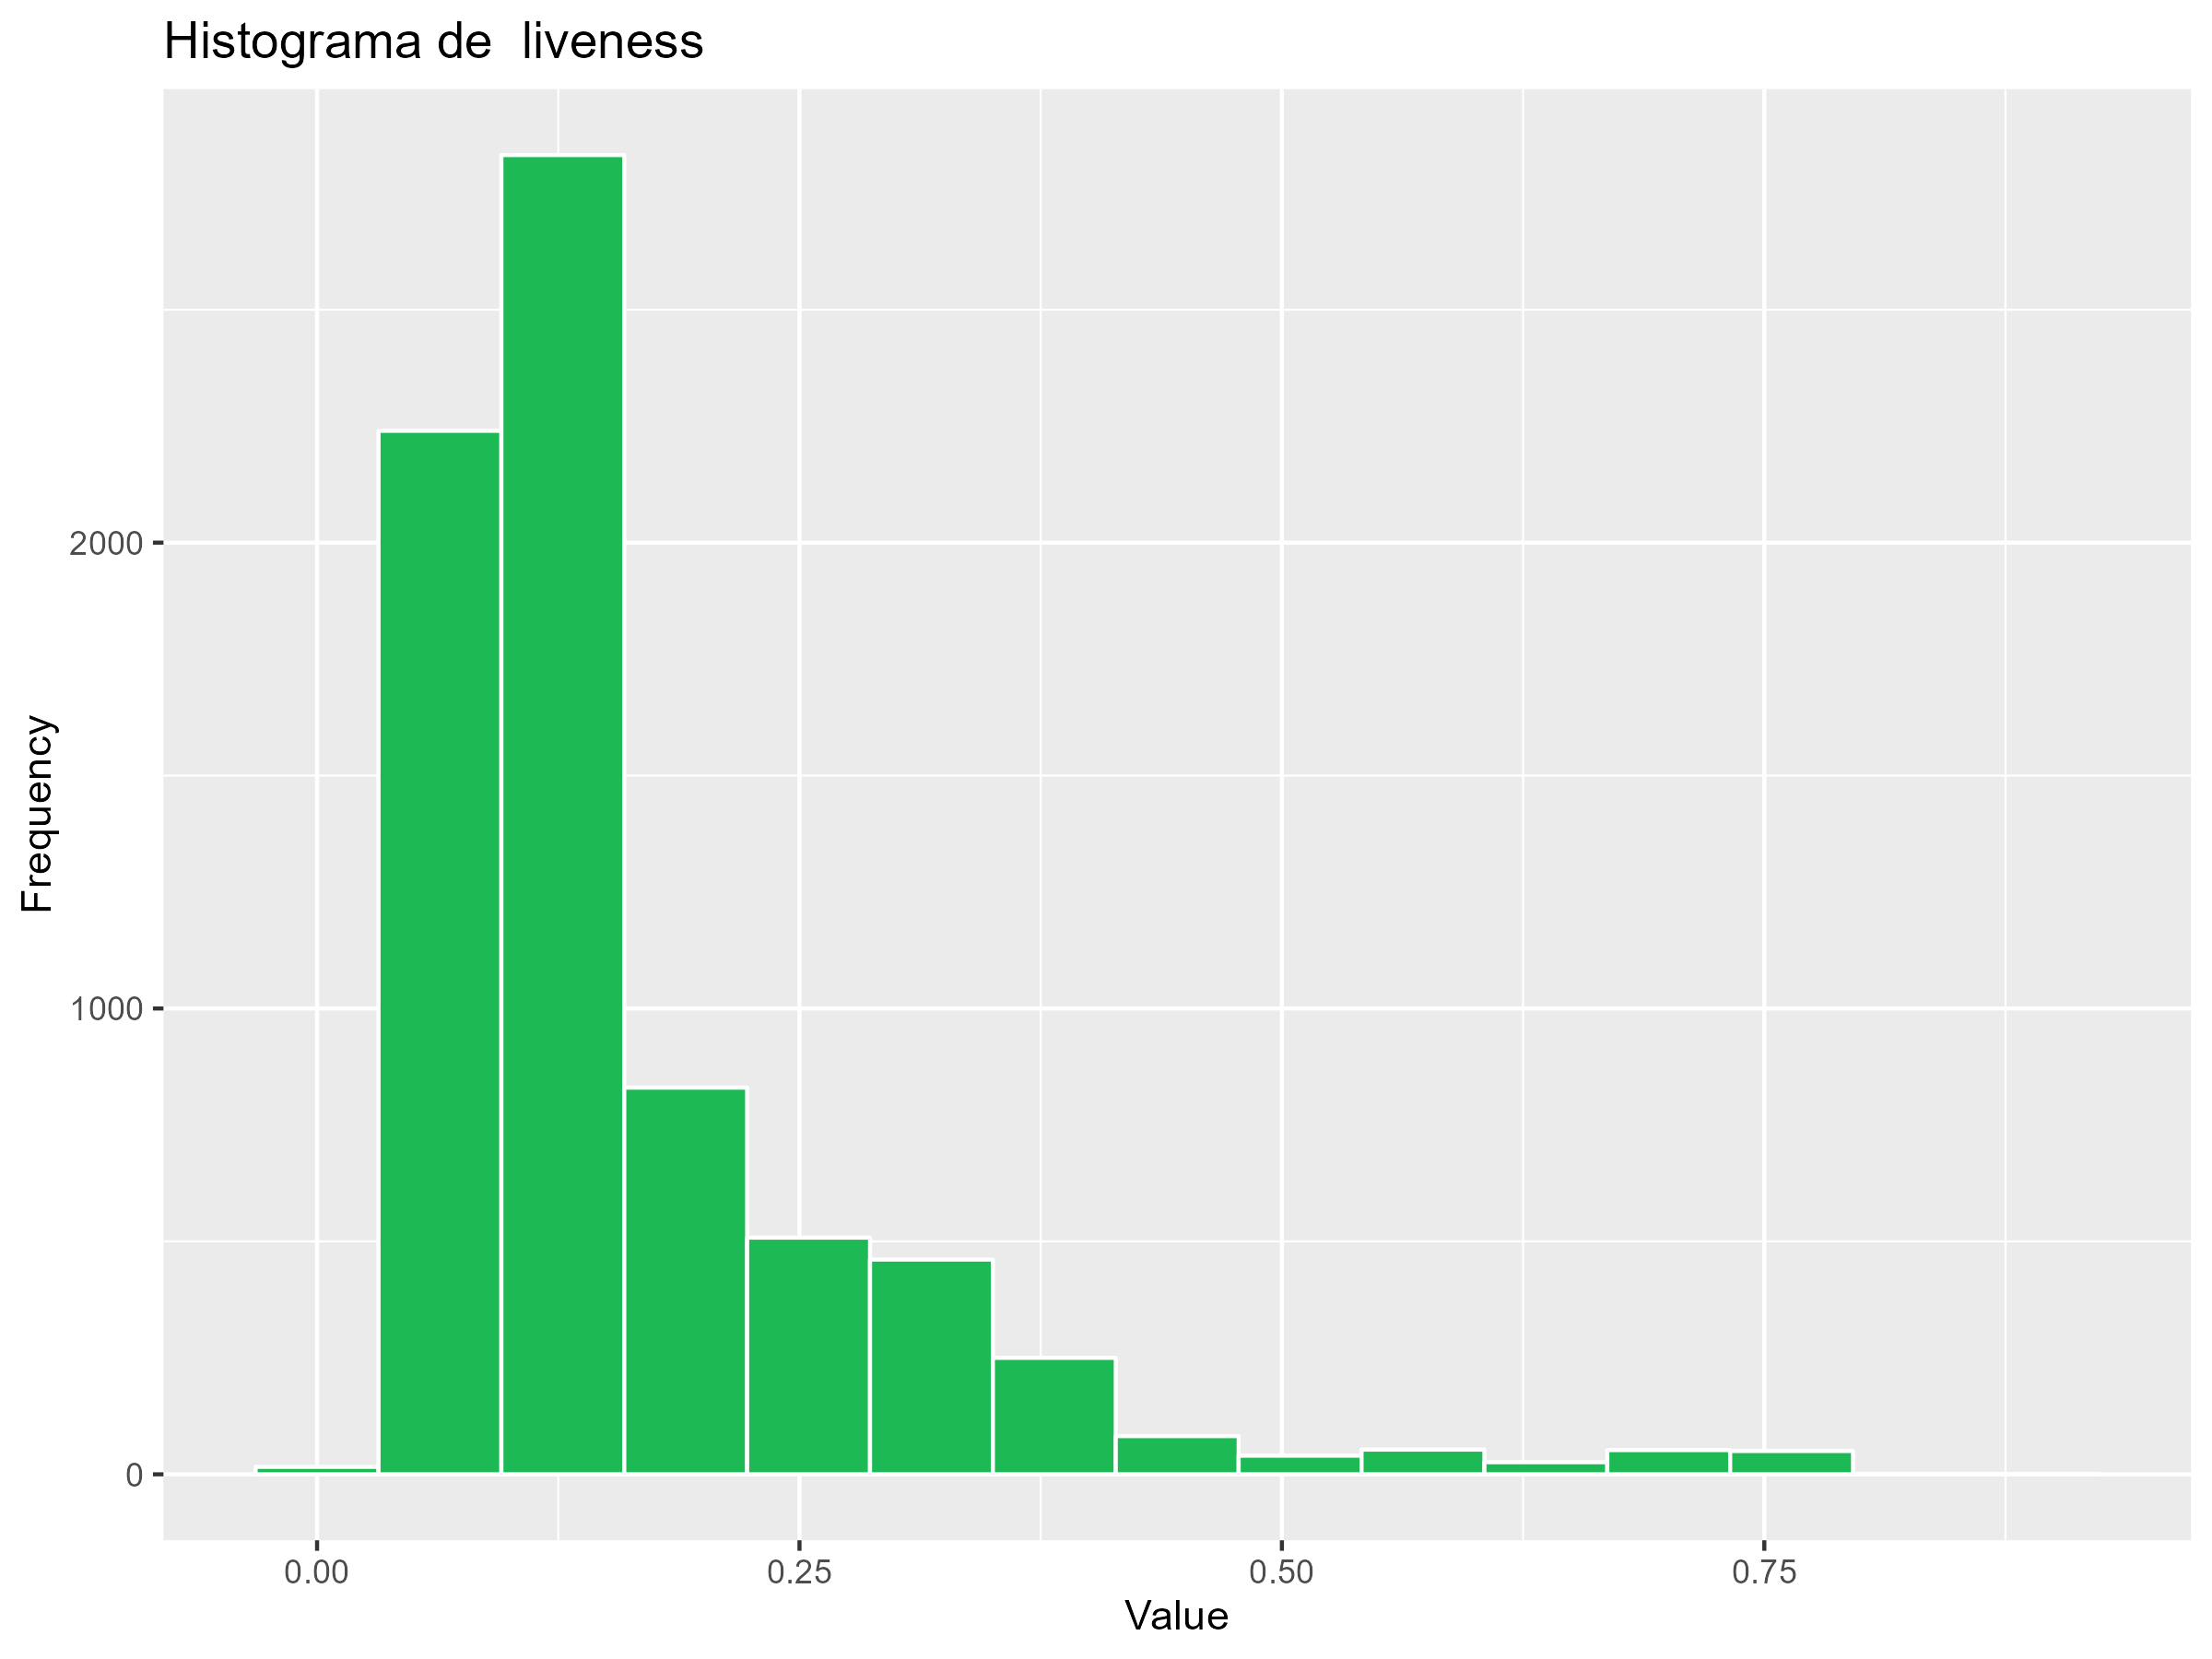
\includegraphics[width=0.95\linewidth]{Images/2_Univariate/hist_liveness.png}
        \caption{Histograma de \textit{liveness}}
        \label{fig:UnivariateR_liveness}
    \end{minipage}%
    \begin{minipage}{.4\textwidth}
        \centering
        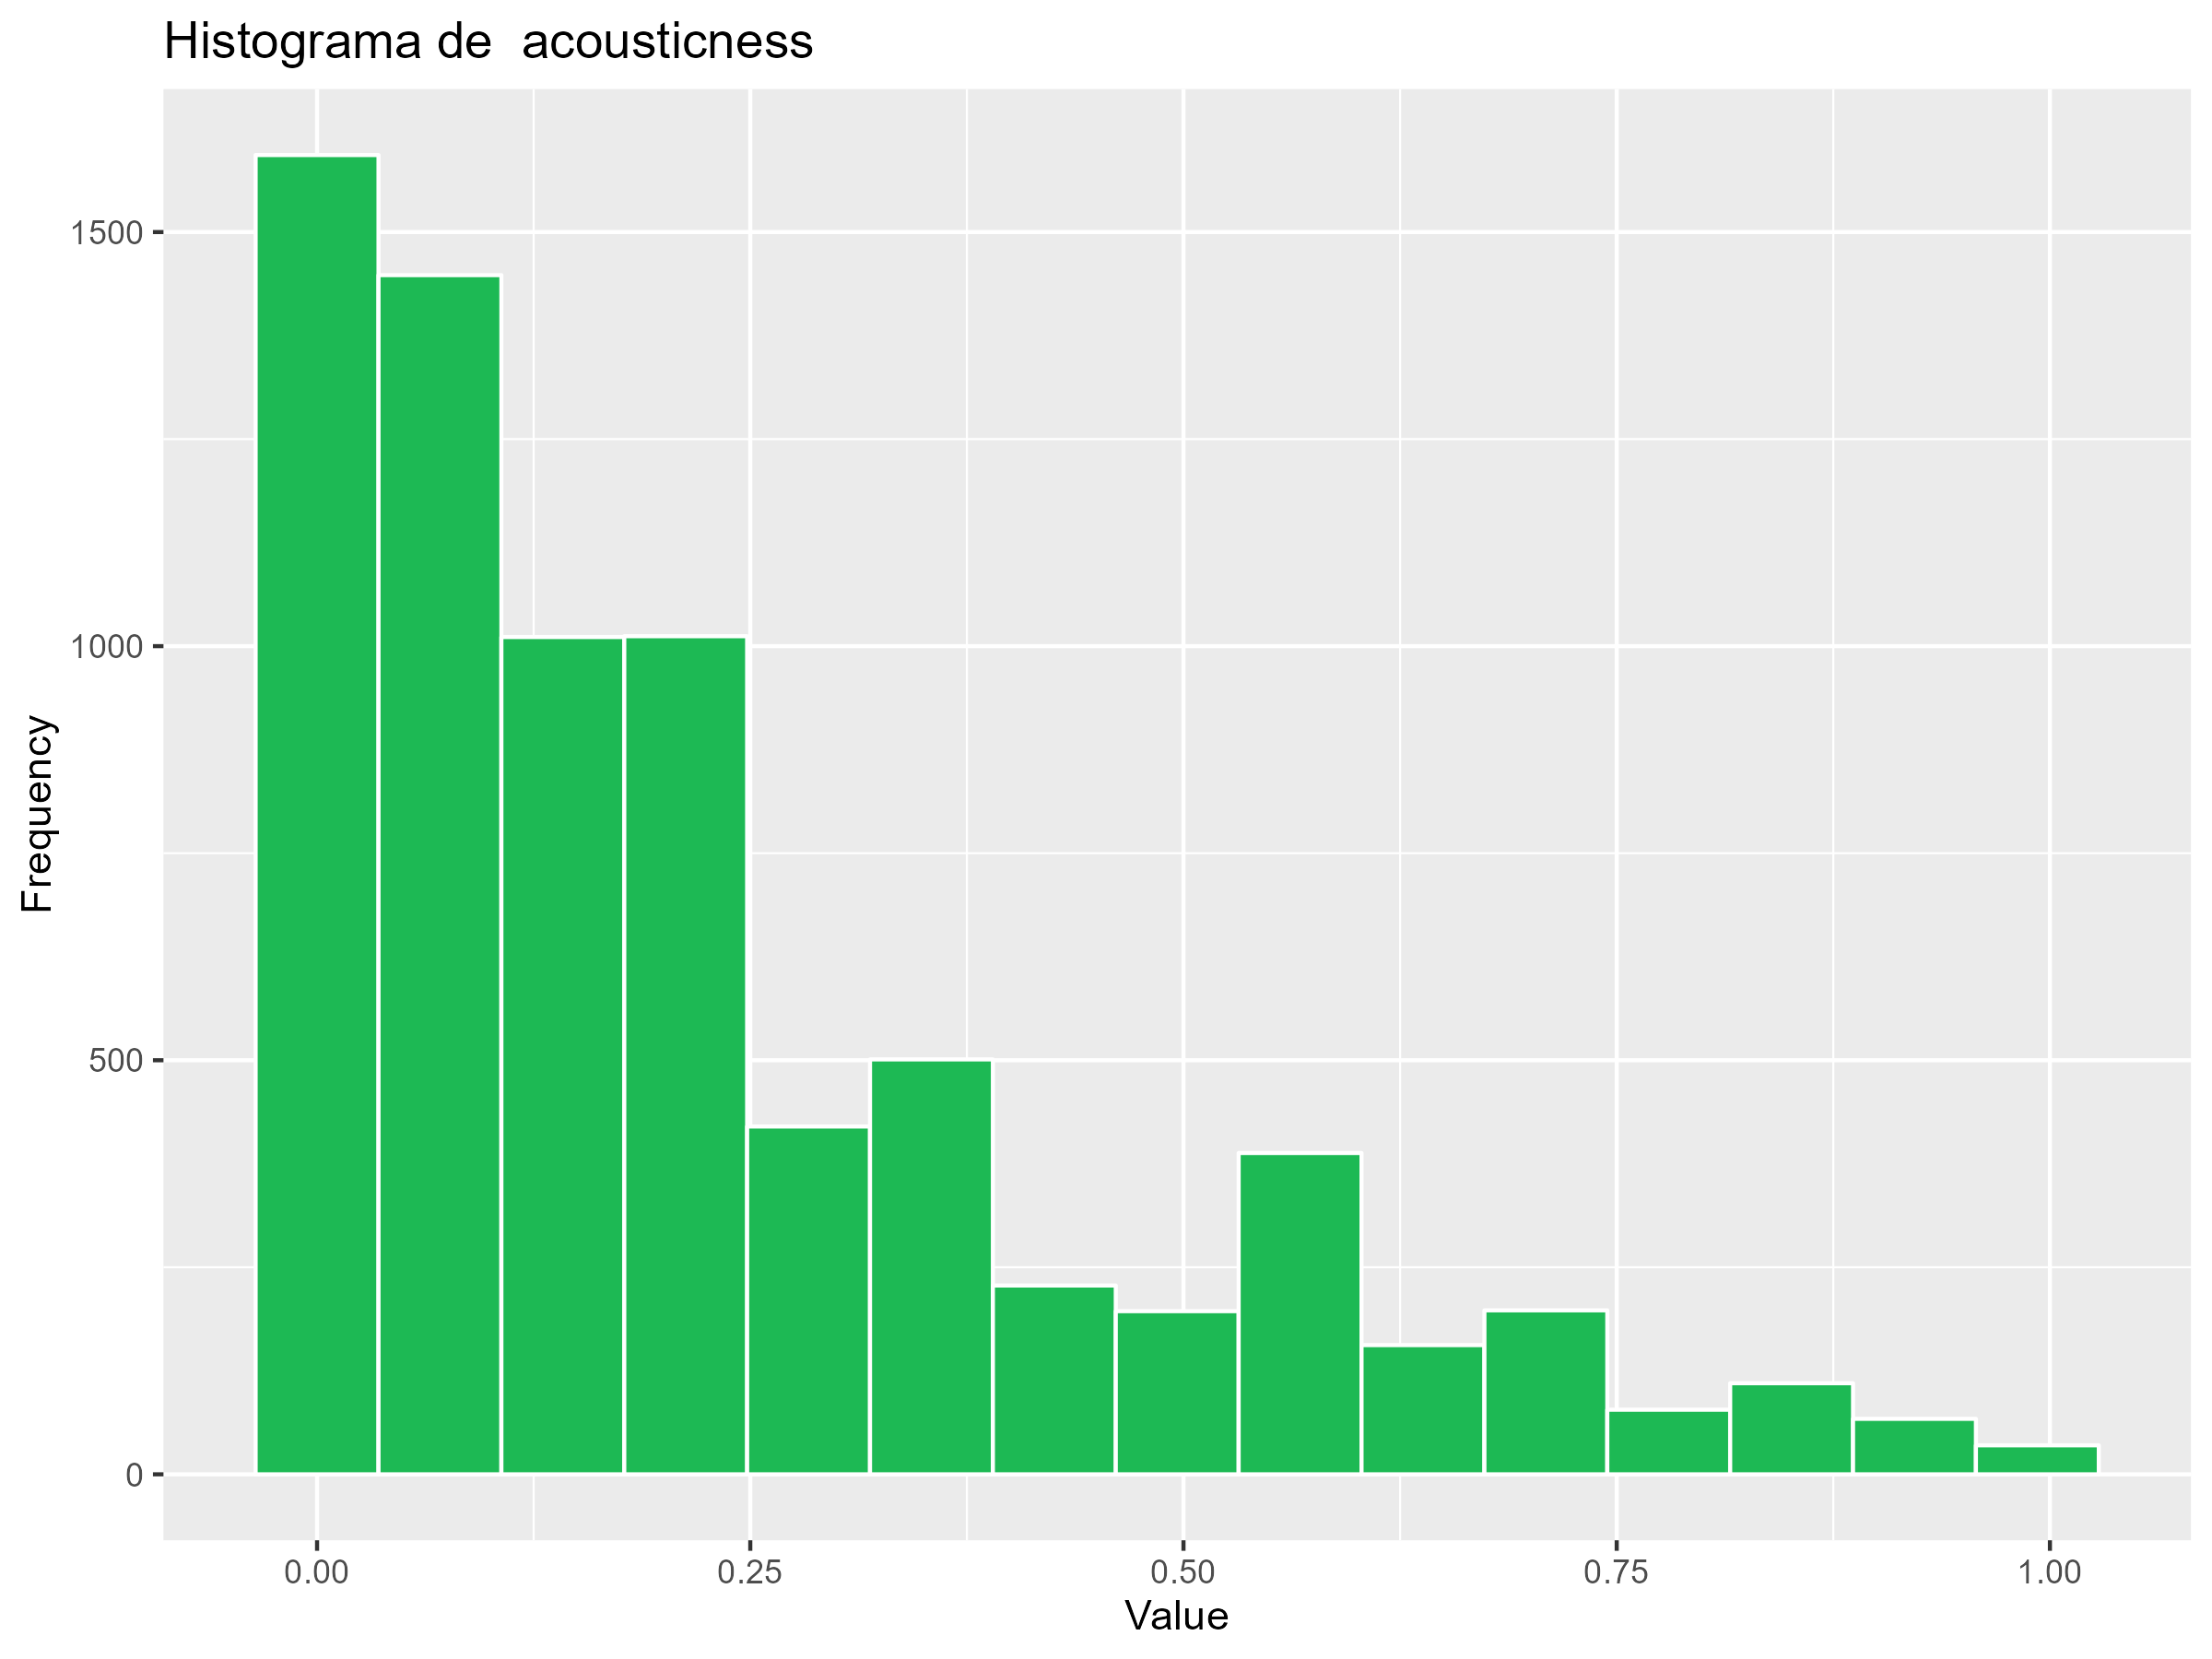
\includegraphics[width=0.95\linewidth]{Images/2_Univariate/hist_acousticness.png}
        \caption{Histograma de \textit{acousticness}}
        \label{fig:UnivariateR_acousticness}
    \end{minipage}%
\end{figure}

Aproximadament la meitat de les aparicions són col·laboracions entre artistes (\ref{fig:UnivariateR_collab}). El 39.2\% de les cançons són explícites (\ref{fig:UnivariateR_explicit}).

\begin{figure}[H]
\centering
    \begin{minipage}{.4\textwidth}
        \centering
        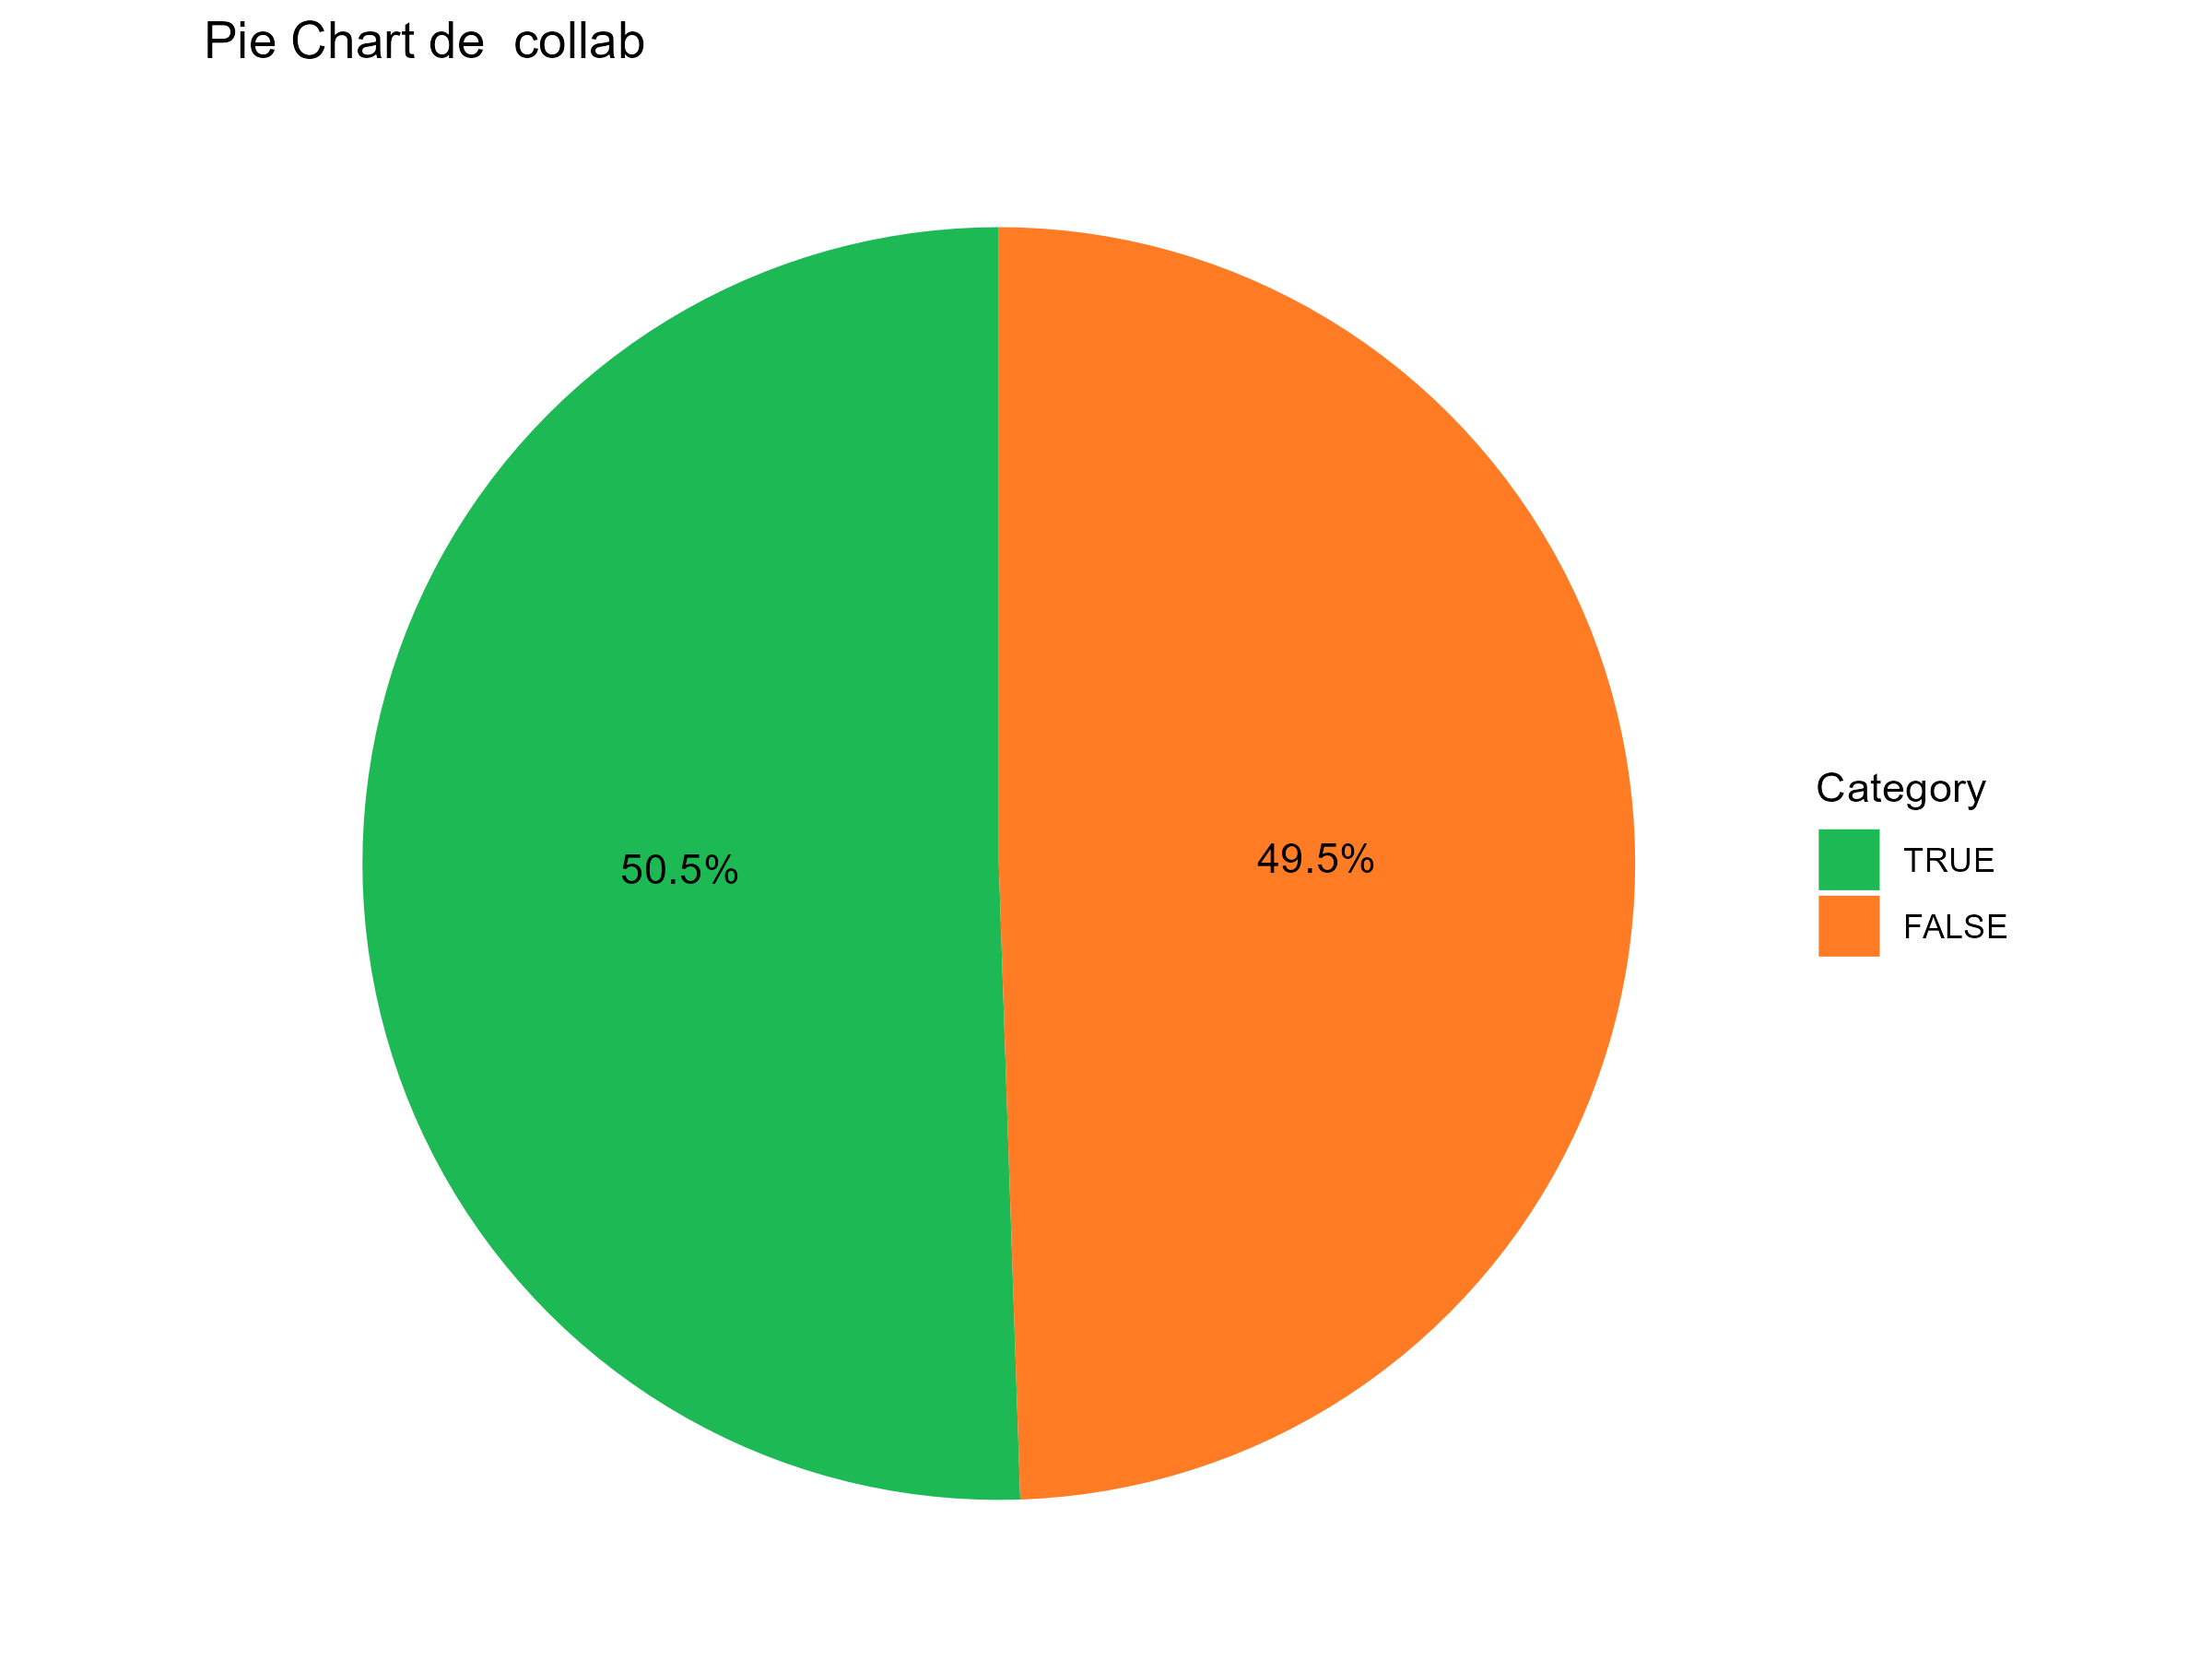
\includegraphics[width=0.95\linewidth]{Images/2_Univariate/pie_collab.png}
        \caption{Pie chart de \textit{collab}}
        \label{fig:UnivariateR_collab}
    \end{minipage}%
    \begin{minipage}{.4\textwidth}
        \centering
        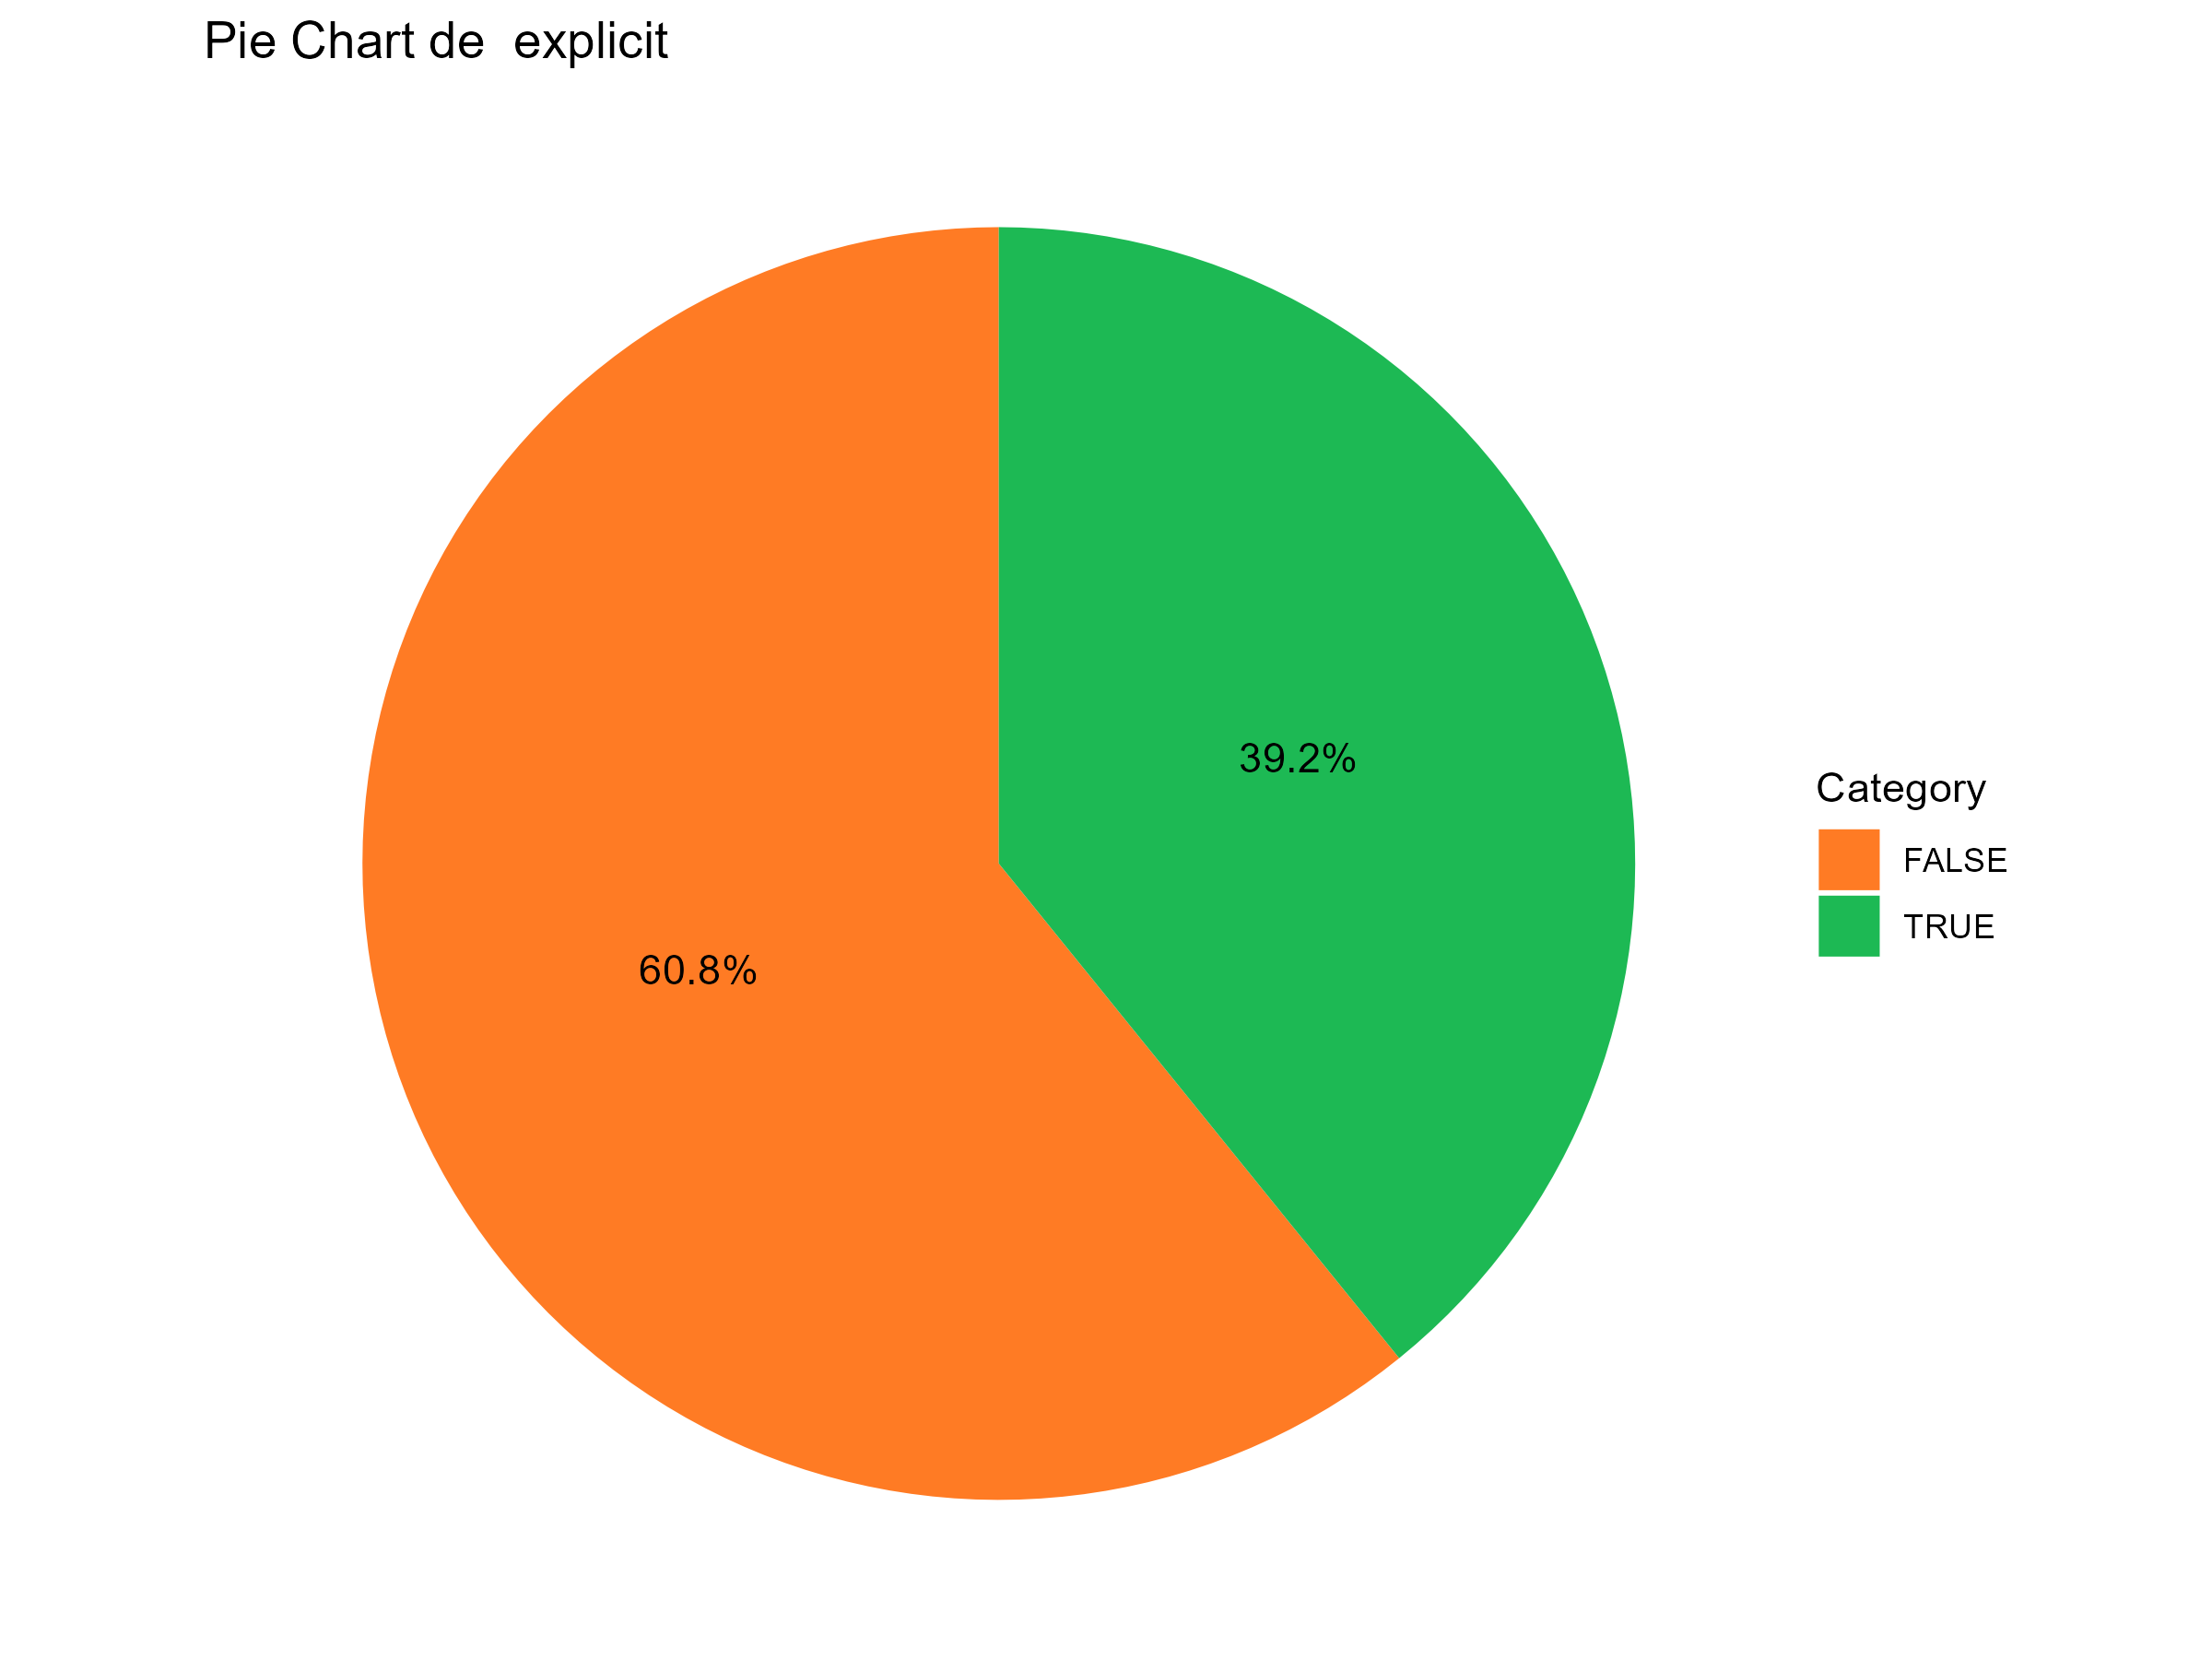
\includegraphics[width=0.95\linewidth]{Images/2_Univariate/pie_explicit.png}
        \caption{Pie chart de \textit{explicit}}
        \label{fig:UnivariateR_explicit}
    \end{minipage}%
\end{figure}

L'any on més cançons es van publicar és el 2018, seguit del 2019, 2017 i 2020 (\ref{fig:UnivariateR_yearrelease}). Aquests coincideixen amb els anys en els que es va analitzar el top de Spotify, o sigui que ens indiquen que aquest top té tendència a contenir cançons recents.

\begin{figure}[H]
    \centering
    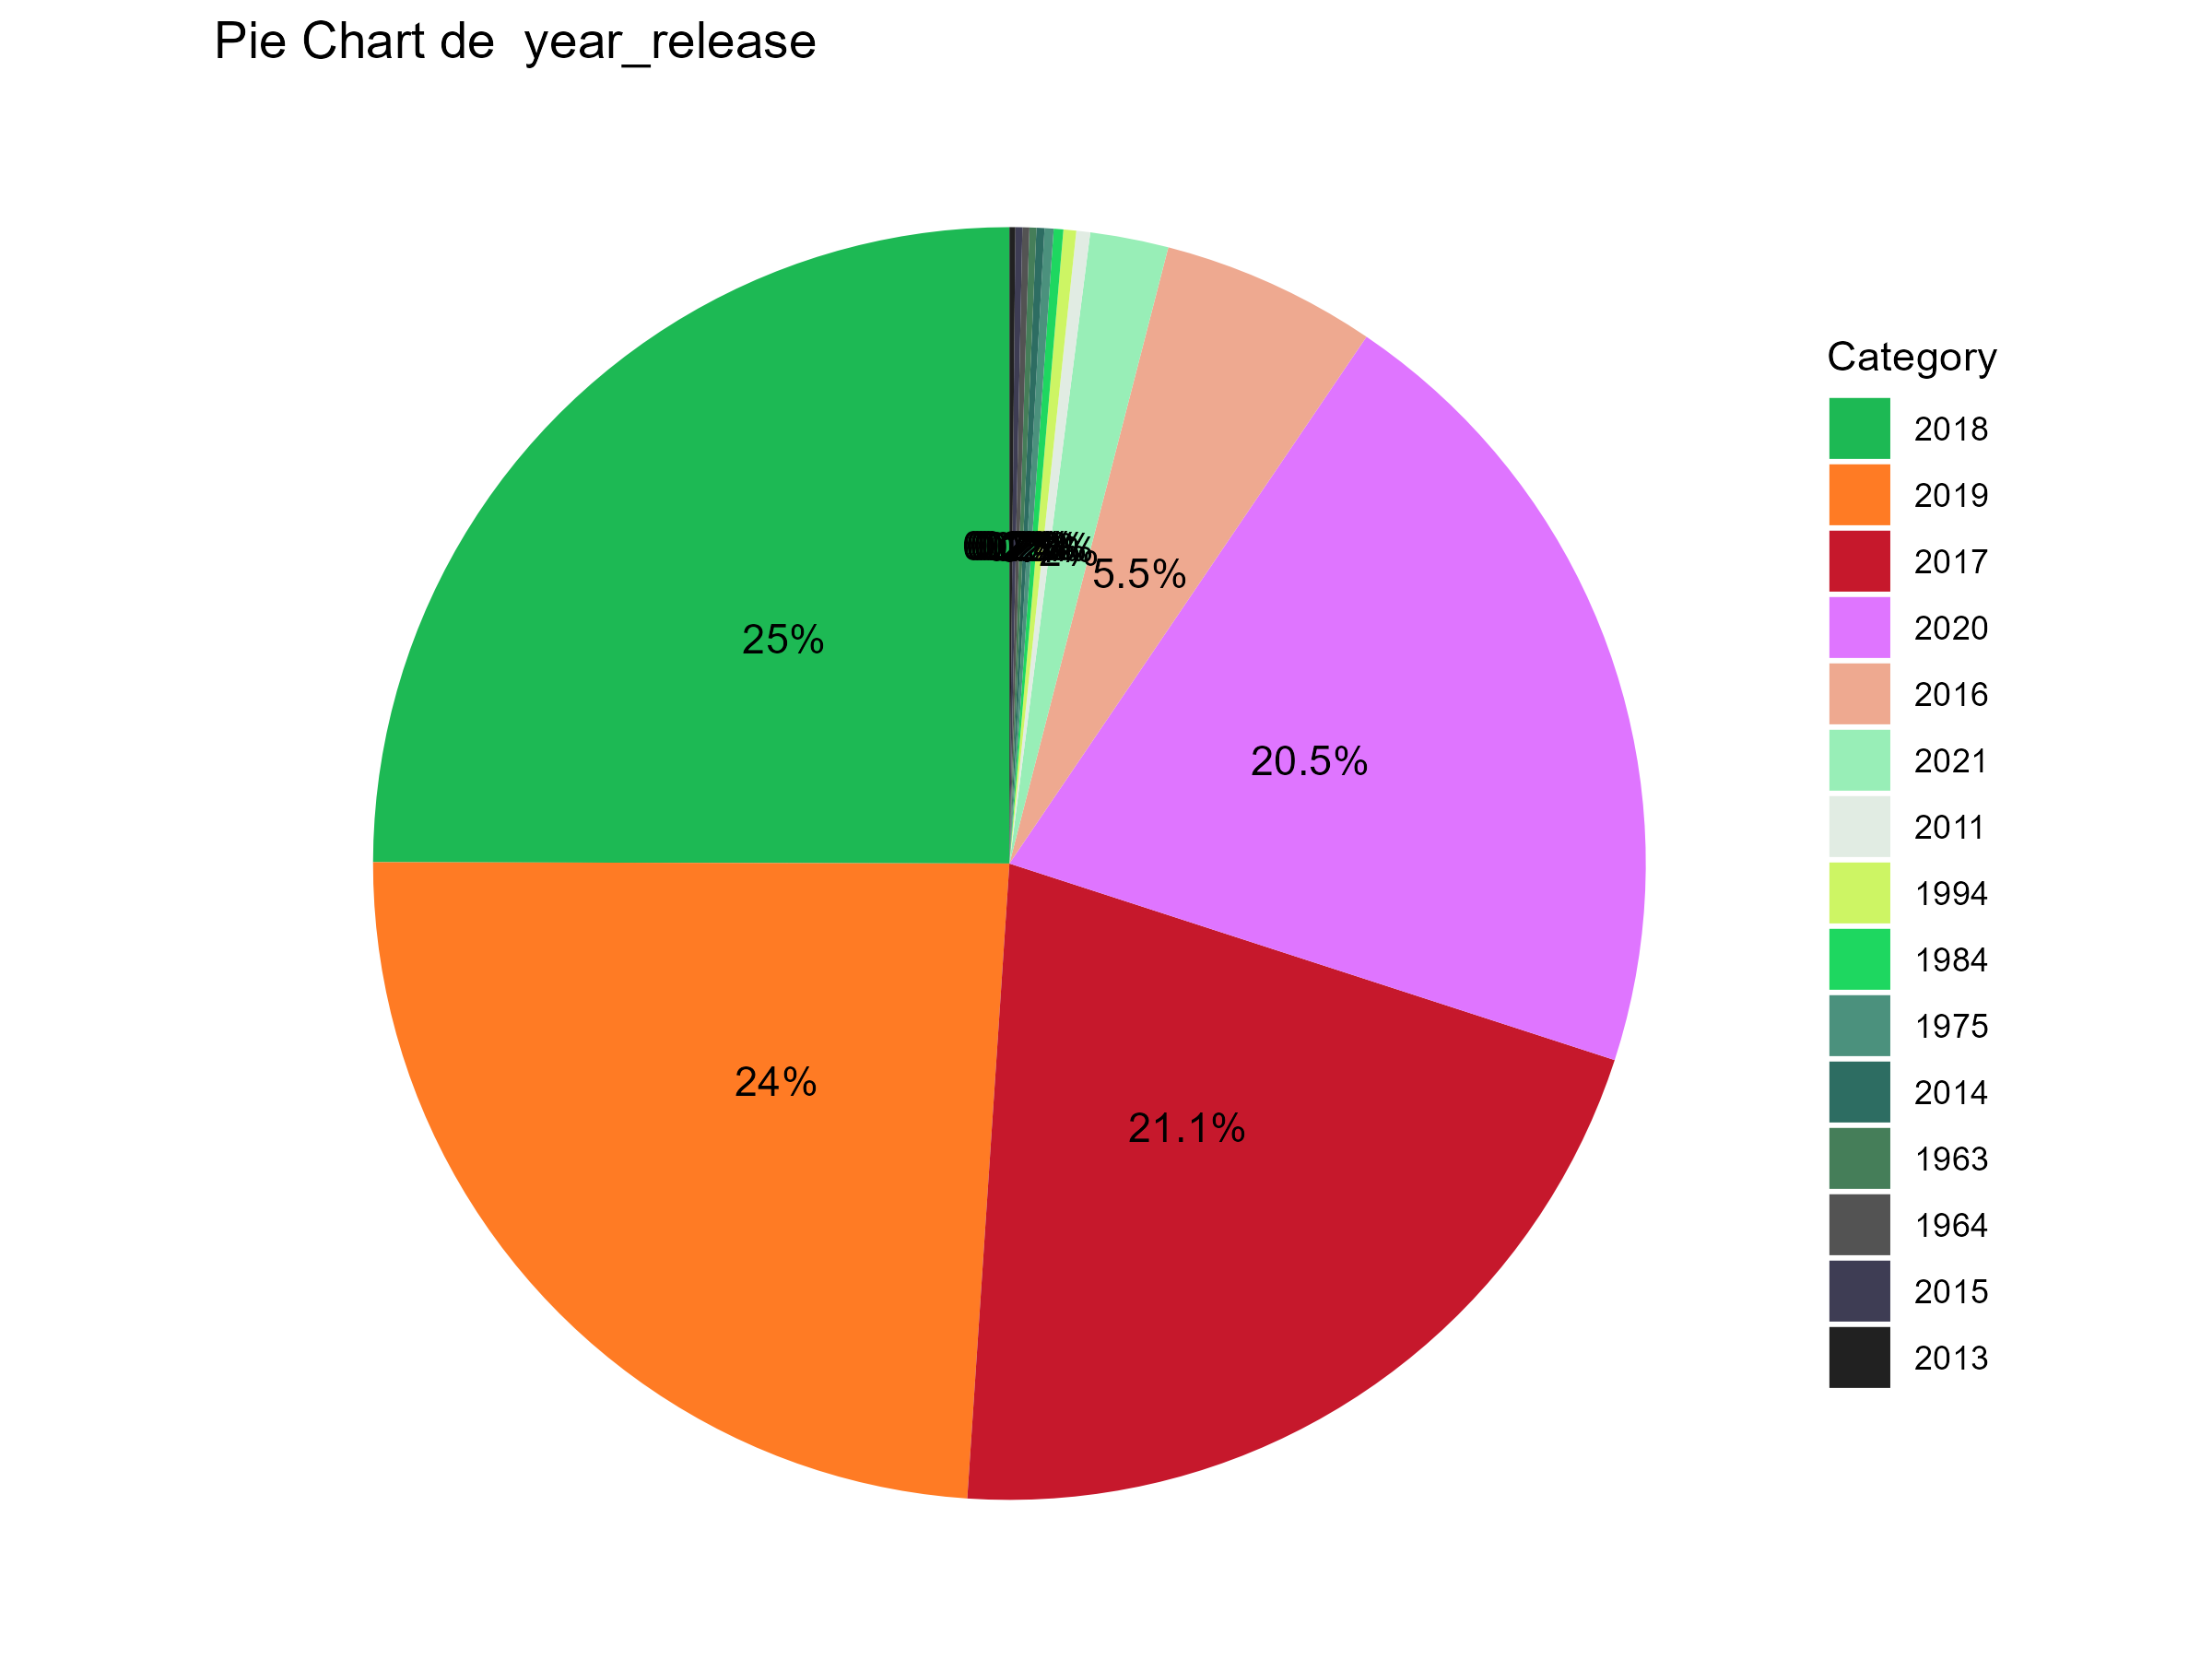
\includegraphics[width=0.8\textwidth]{Images/2_Univariate/pie_year_release.png}
    \caption{Pie chart de \textit{year\_release}}
    \label{fig:UnivariateR_yearrelease}
\end{figure}

Observant les variables noves, que comentarem com es van obtenir més endavant, veiem que el país amb més representació (amb molta diferència) és els Estats Units d'Amèrica, amb 3990 aparicions (\ref{fig:UnivariateR_nationality}). Tot i això, detectem algun problema en aquest dataset (sense processar), ja que per exemple diferencia United Kingdom de England i Scotland. Un altre problema és amb city, que a vegades apareixen països com a nom de ciutat en els artistes amb doble nacionalitat (\ref{fig:UnivariateR_city}). La ciutat amb més aparicions és San Juan.

\begin{figure}[H]
\centering
    \begin{minipage}{.4\textwidth}
        \centering
        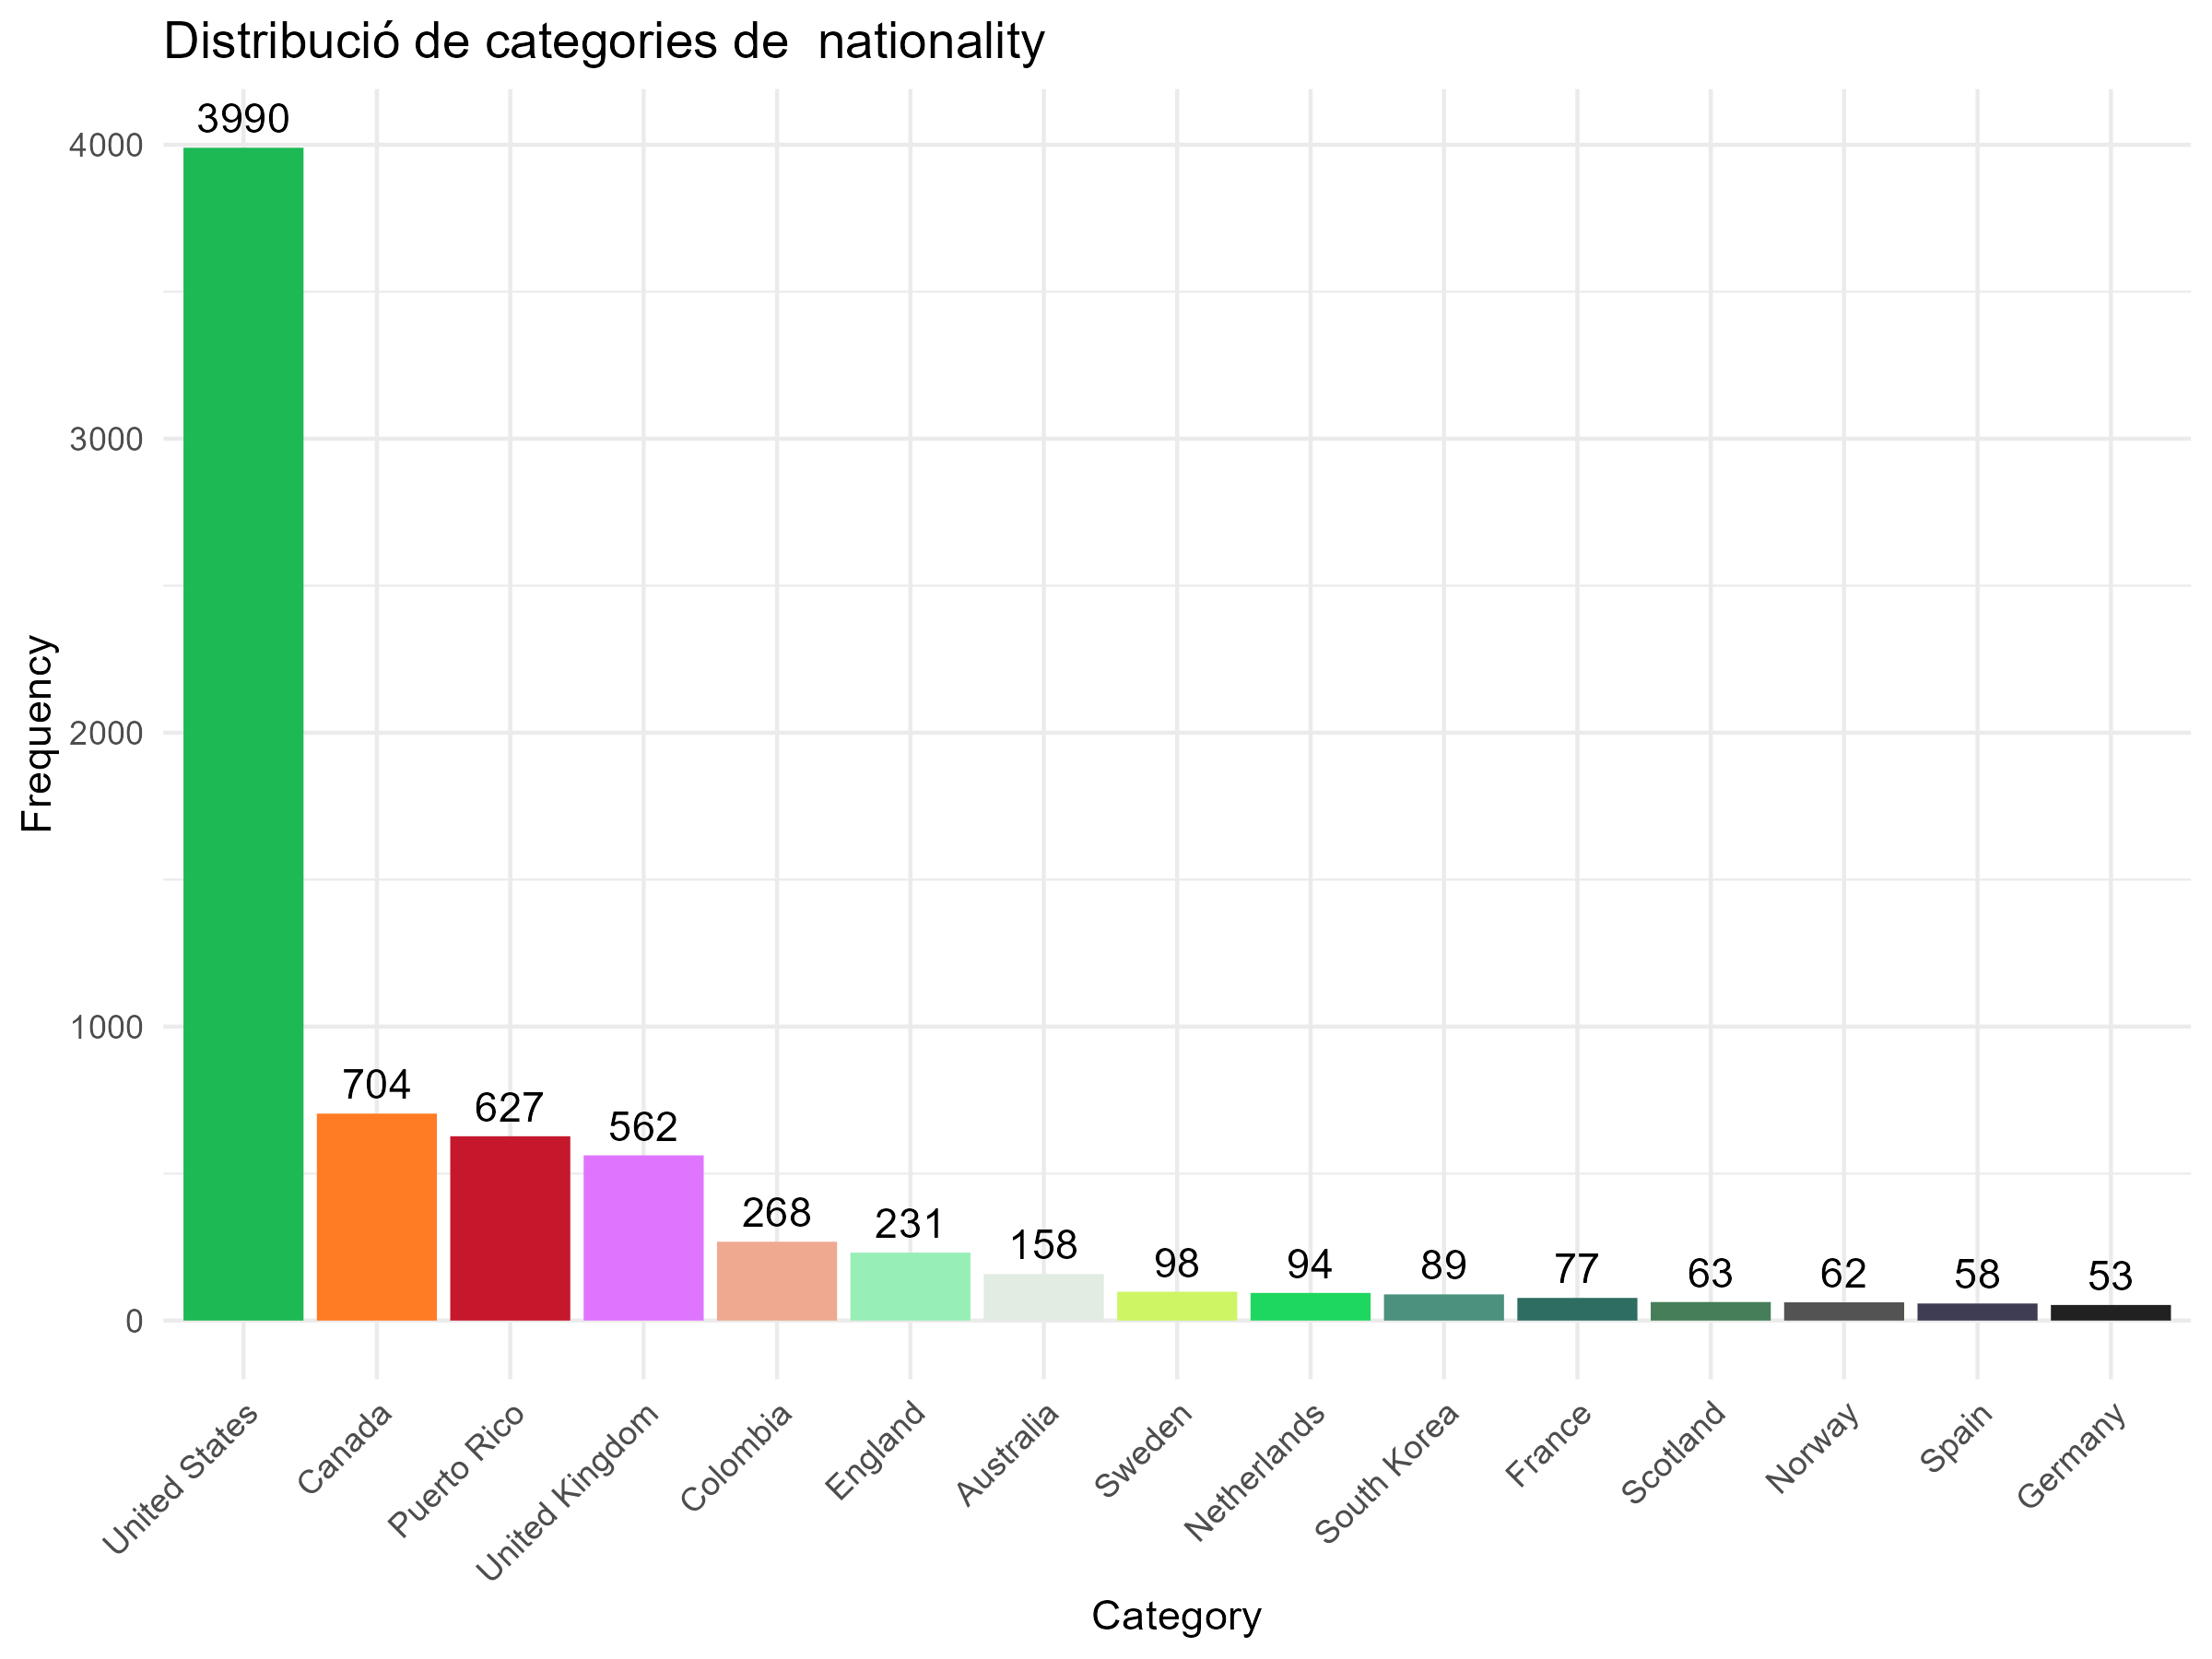
\includegraphics[width=0.95\linewidth]{Images/2_Univariate/bar_nationality.png}
        \caption{Bar plot de \textit{nationality}}
        \label{fig:UnivariateR_nationality}
    \end{minipage}%
    \begin{minipage}{.4\textwidth}
        \centering
        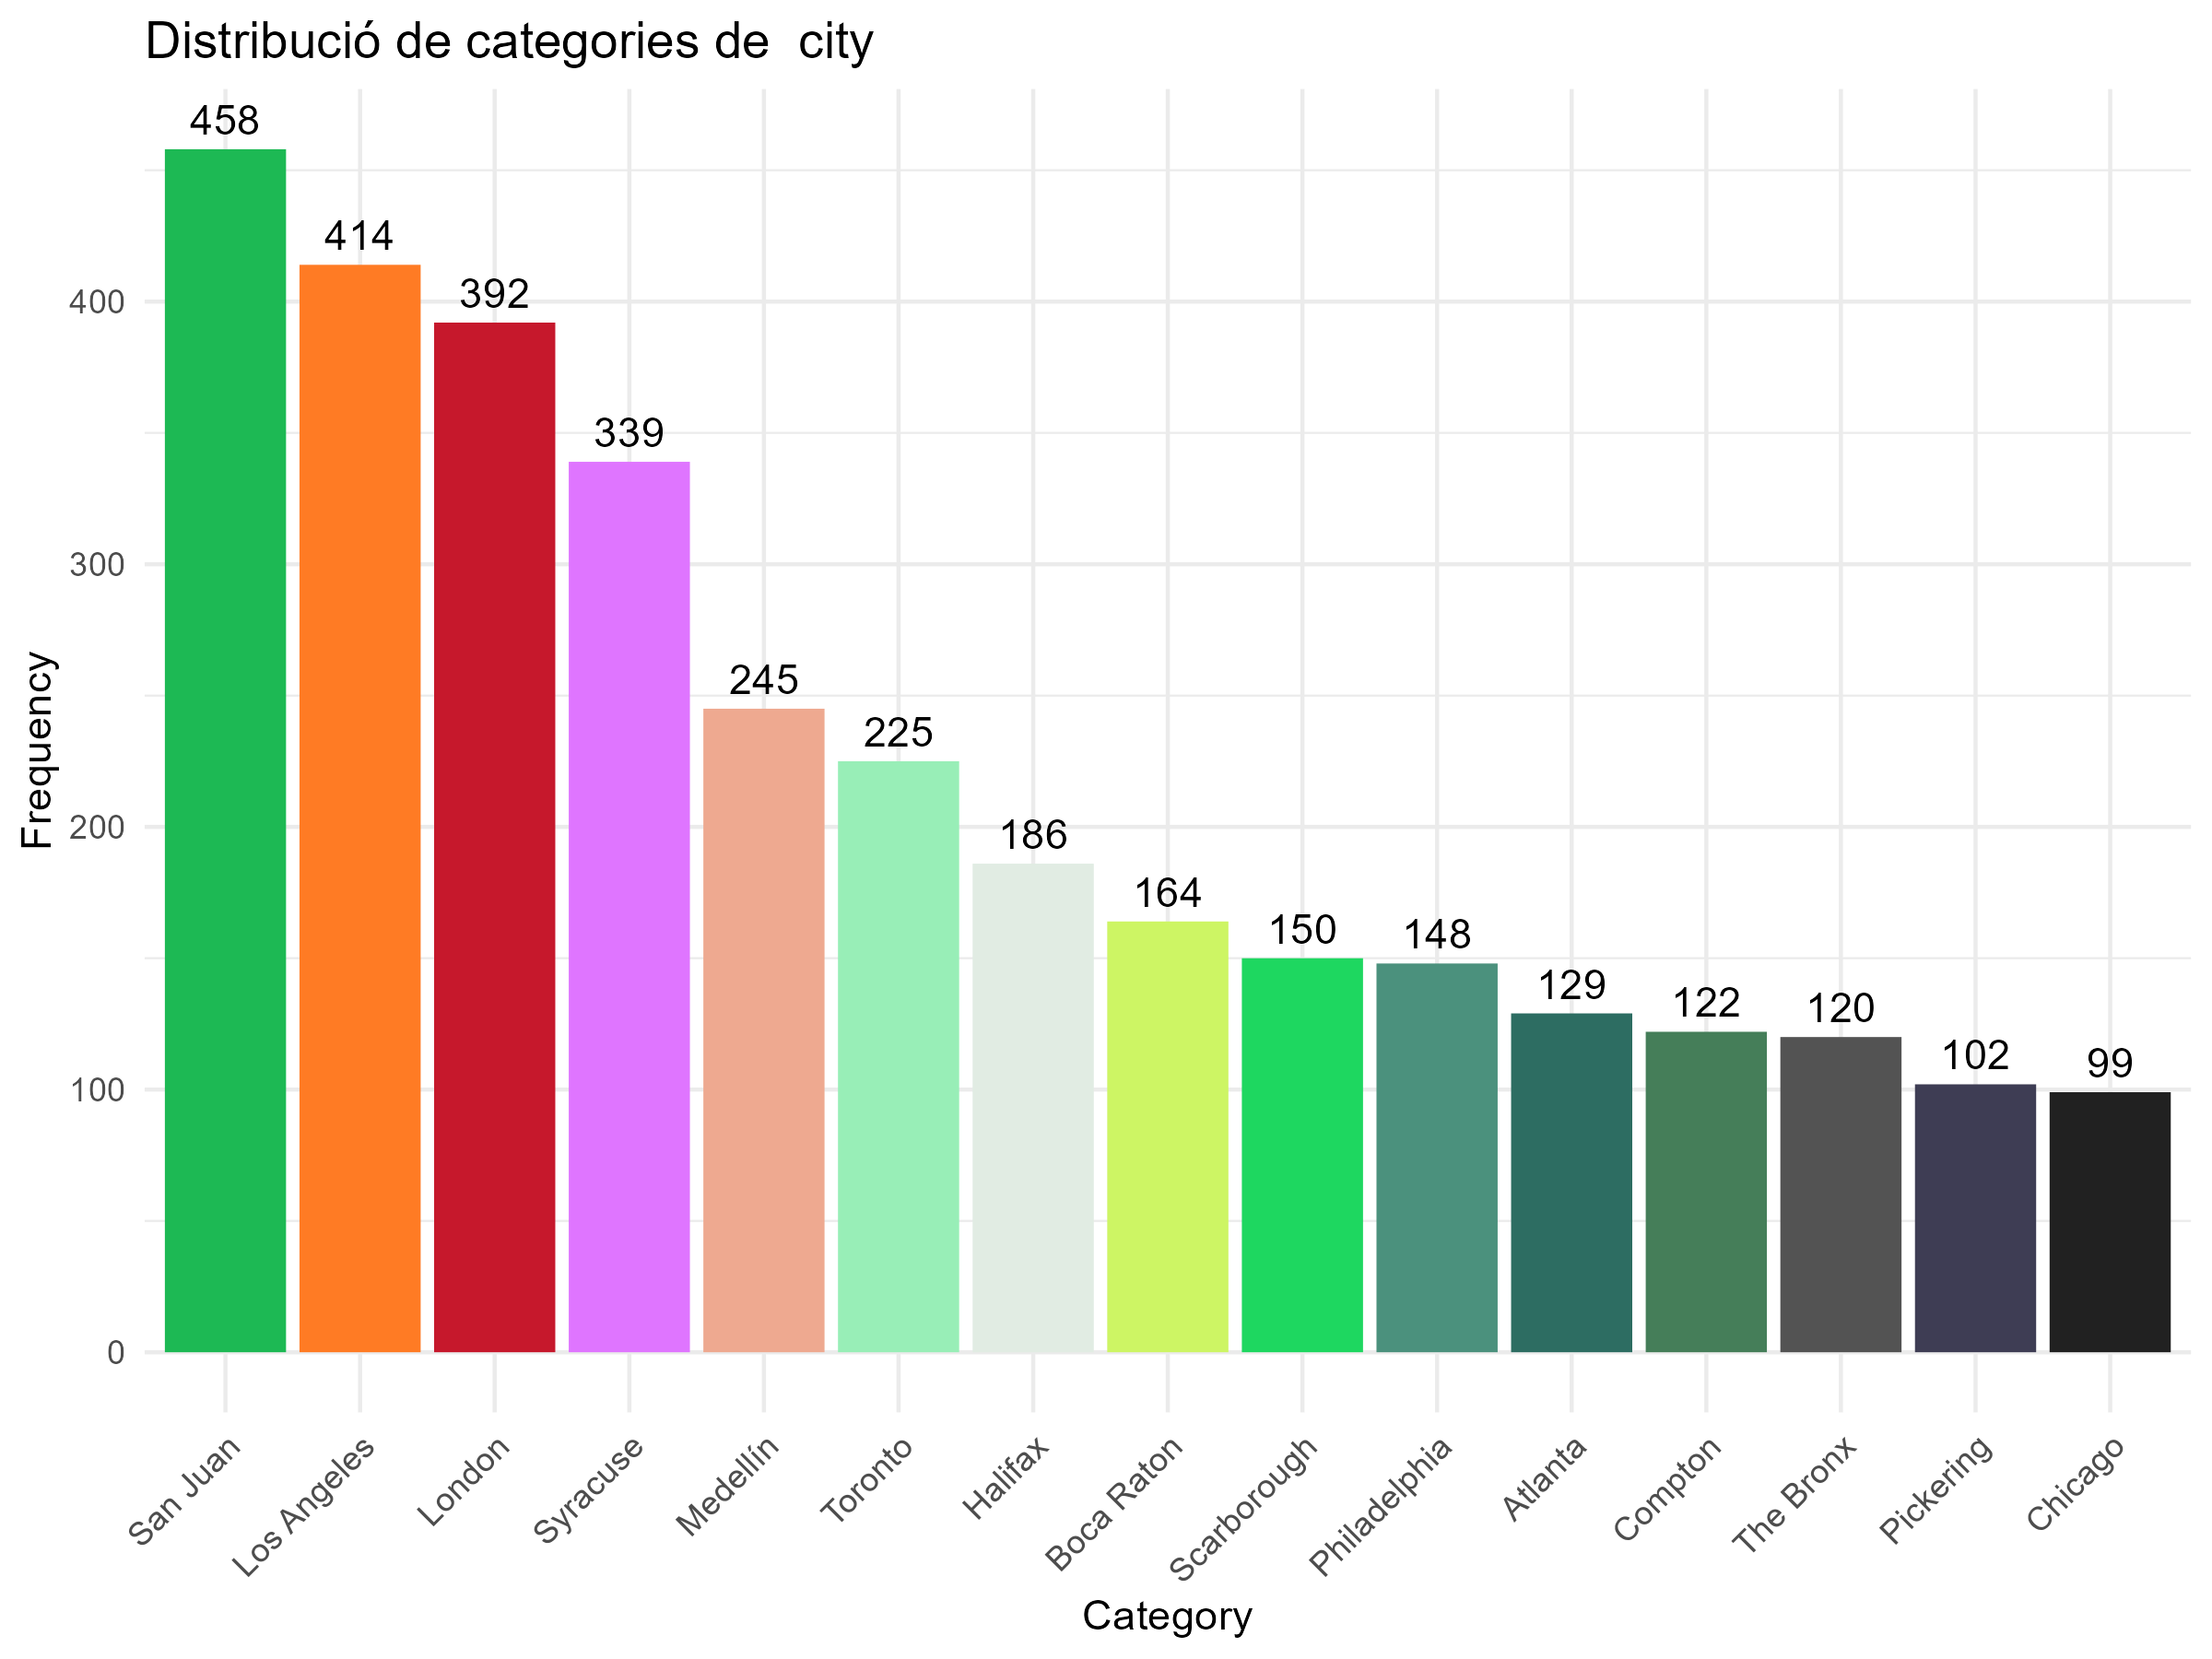
\includegraphics[width=0.95\linewidth]{Images/2_Univariate/bar_city.png}
        \caption{Bar plot de \textit{city}}
        \label{fig:UnivariateR_city}
    \end{minipage}%
\end{figure}

Analitzant el gènere, observem una clar predomini dels artistes del gènere masculí, apareixent un 72.9\% dels cops (\ref{fig:UnivariateR_gender}). A més, tan sols el 9.3\% dels artistes són grups (\ref{fig:UnivariateR_group}).

\begin{figure}[H]
\centering
    \begin{minipage}{.4\textwidth}
        \centering
        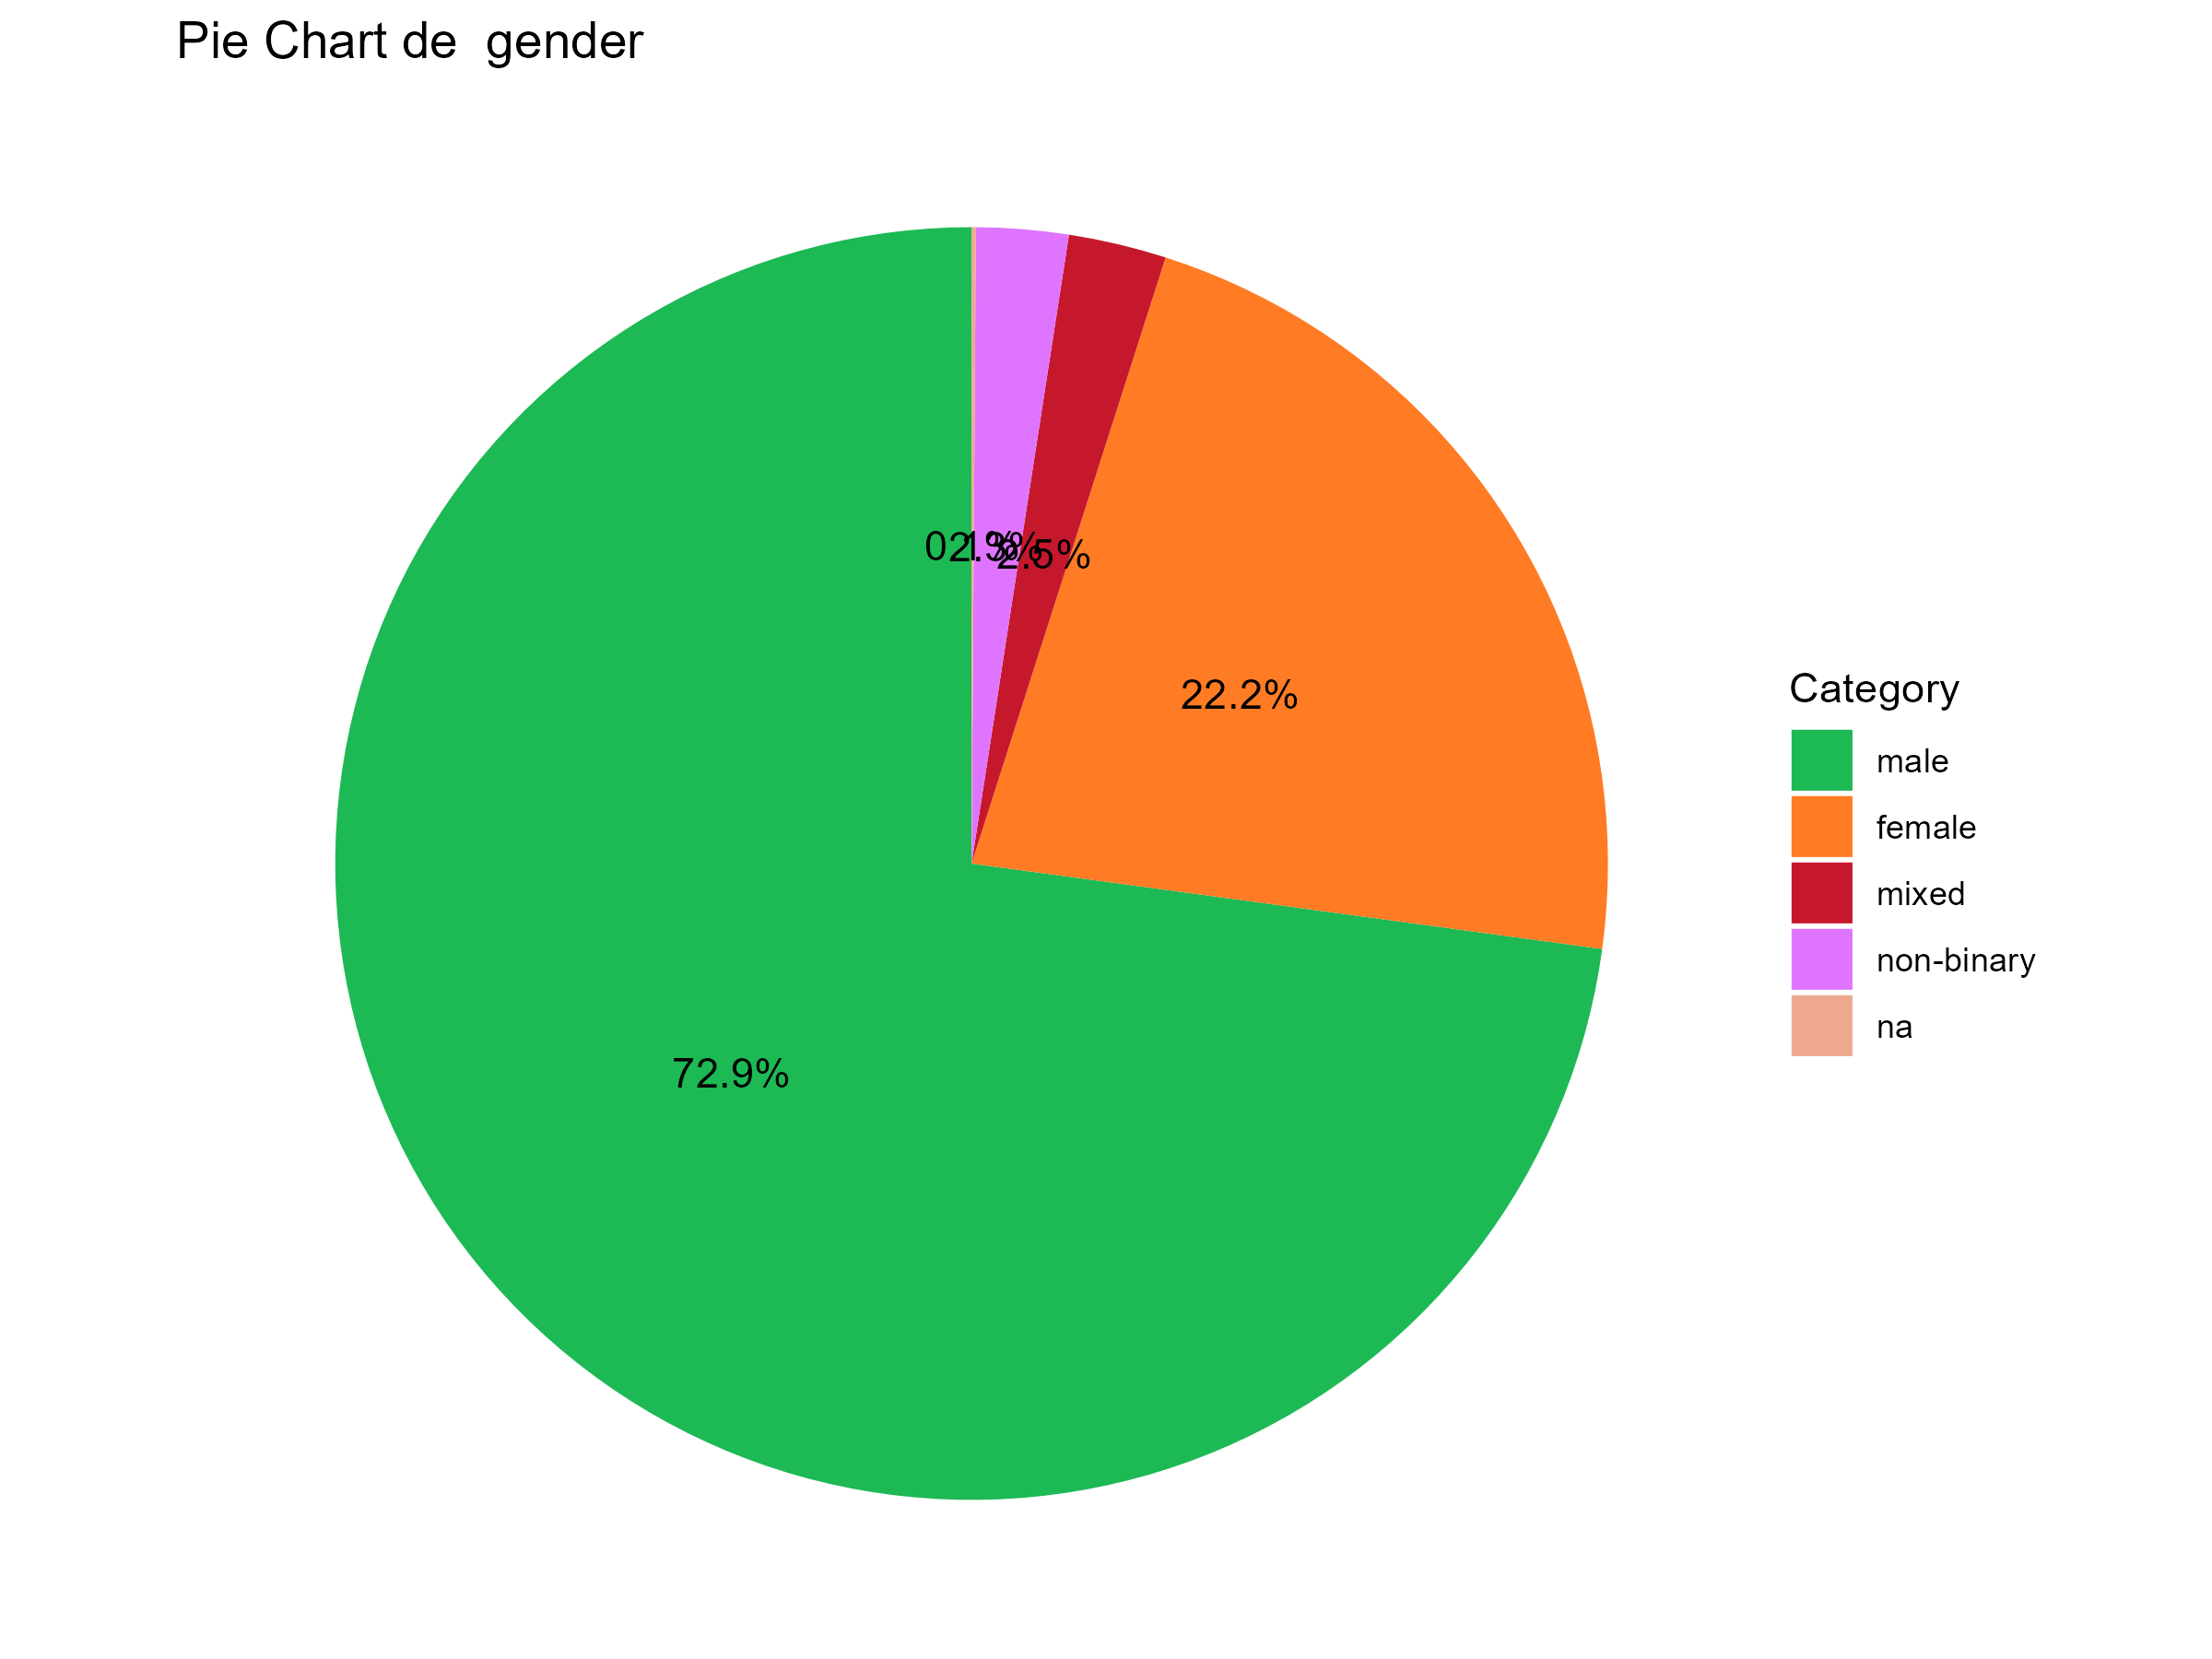
\includegraphics[width=0.95\linewidth]{Images/2_Univariate/pie_gender.png}
        \caption{Pie plot de \textit{gender}}
        \label{fig:UnivariateR_gender}
    \end{minipage}%
    \begin{minipage}{.4\textwidth}
        \centering
        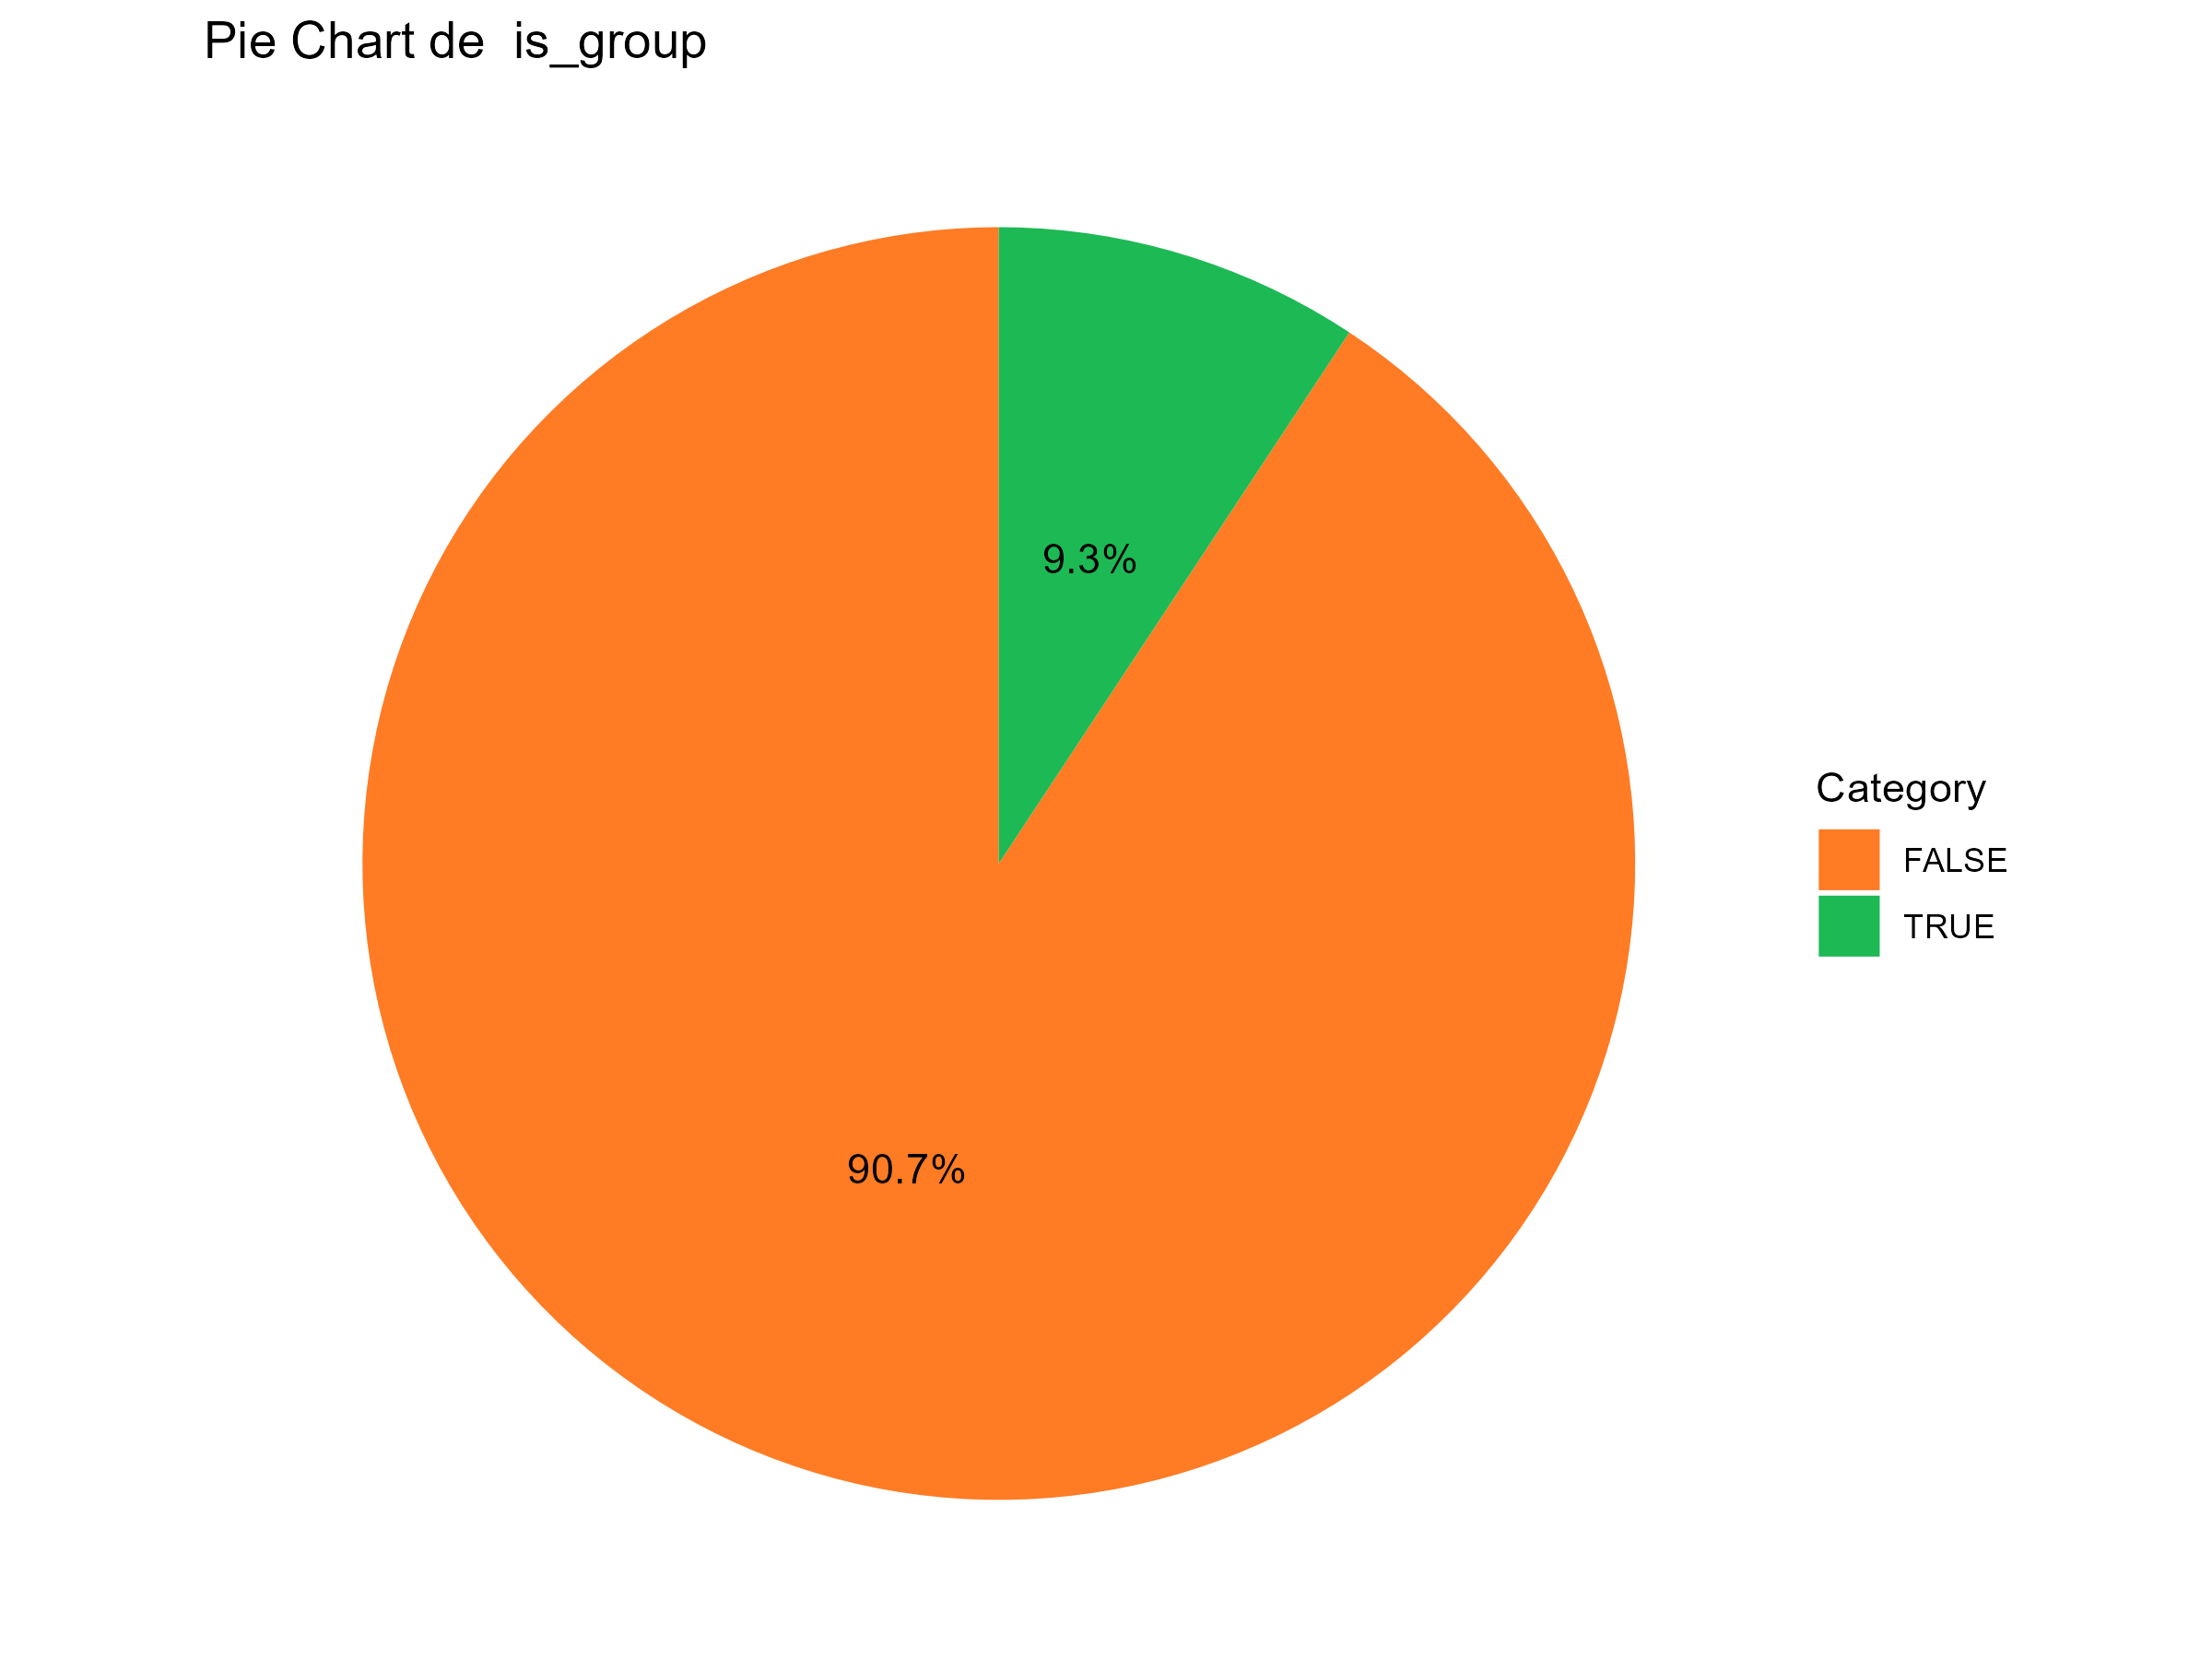
\includegraphics[width=0.95\linewidth]{Images/2_Univariate/pie_is_group.png}
        \caption{Pie plot de \textit{is\_group}}
        \label{fig:UnivariateR_group}
    \end{minipage}%
\end{figure}

Algunes de les variables, però, encara contenen algun problema (sobretot les provinents de la API). Per exemple, hi ha categòriques amb missing data, o les ciutats que hem comentat. A l'apartat de preprocessing, s'afegiran NA a les variables numèriques, s'imputaran i també s'intentaran arreglar aquests errors.

\subsection{Anàlisi bivariant}

L’anàlisi descriptiu bivariant en el passat s'havia realitzat tan sols d’una petita selecció de variables, mentre que en aquest cas s’ha optat per fer-ho amb pràcticament totes. En el fitxer de resultats s’ha evitat incloure album popularity perquè estava molt relacionat amb track popularity, com es pot observar a continuació (figura \ref{fig:BivariateR_trackalbum}):

\begin{figure}[H]
    \centering
    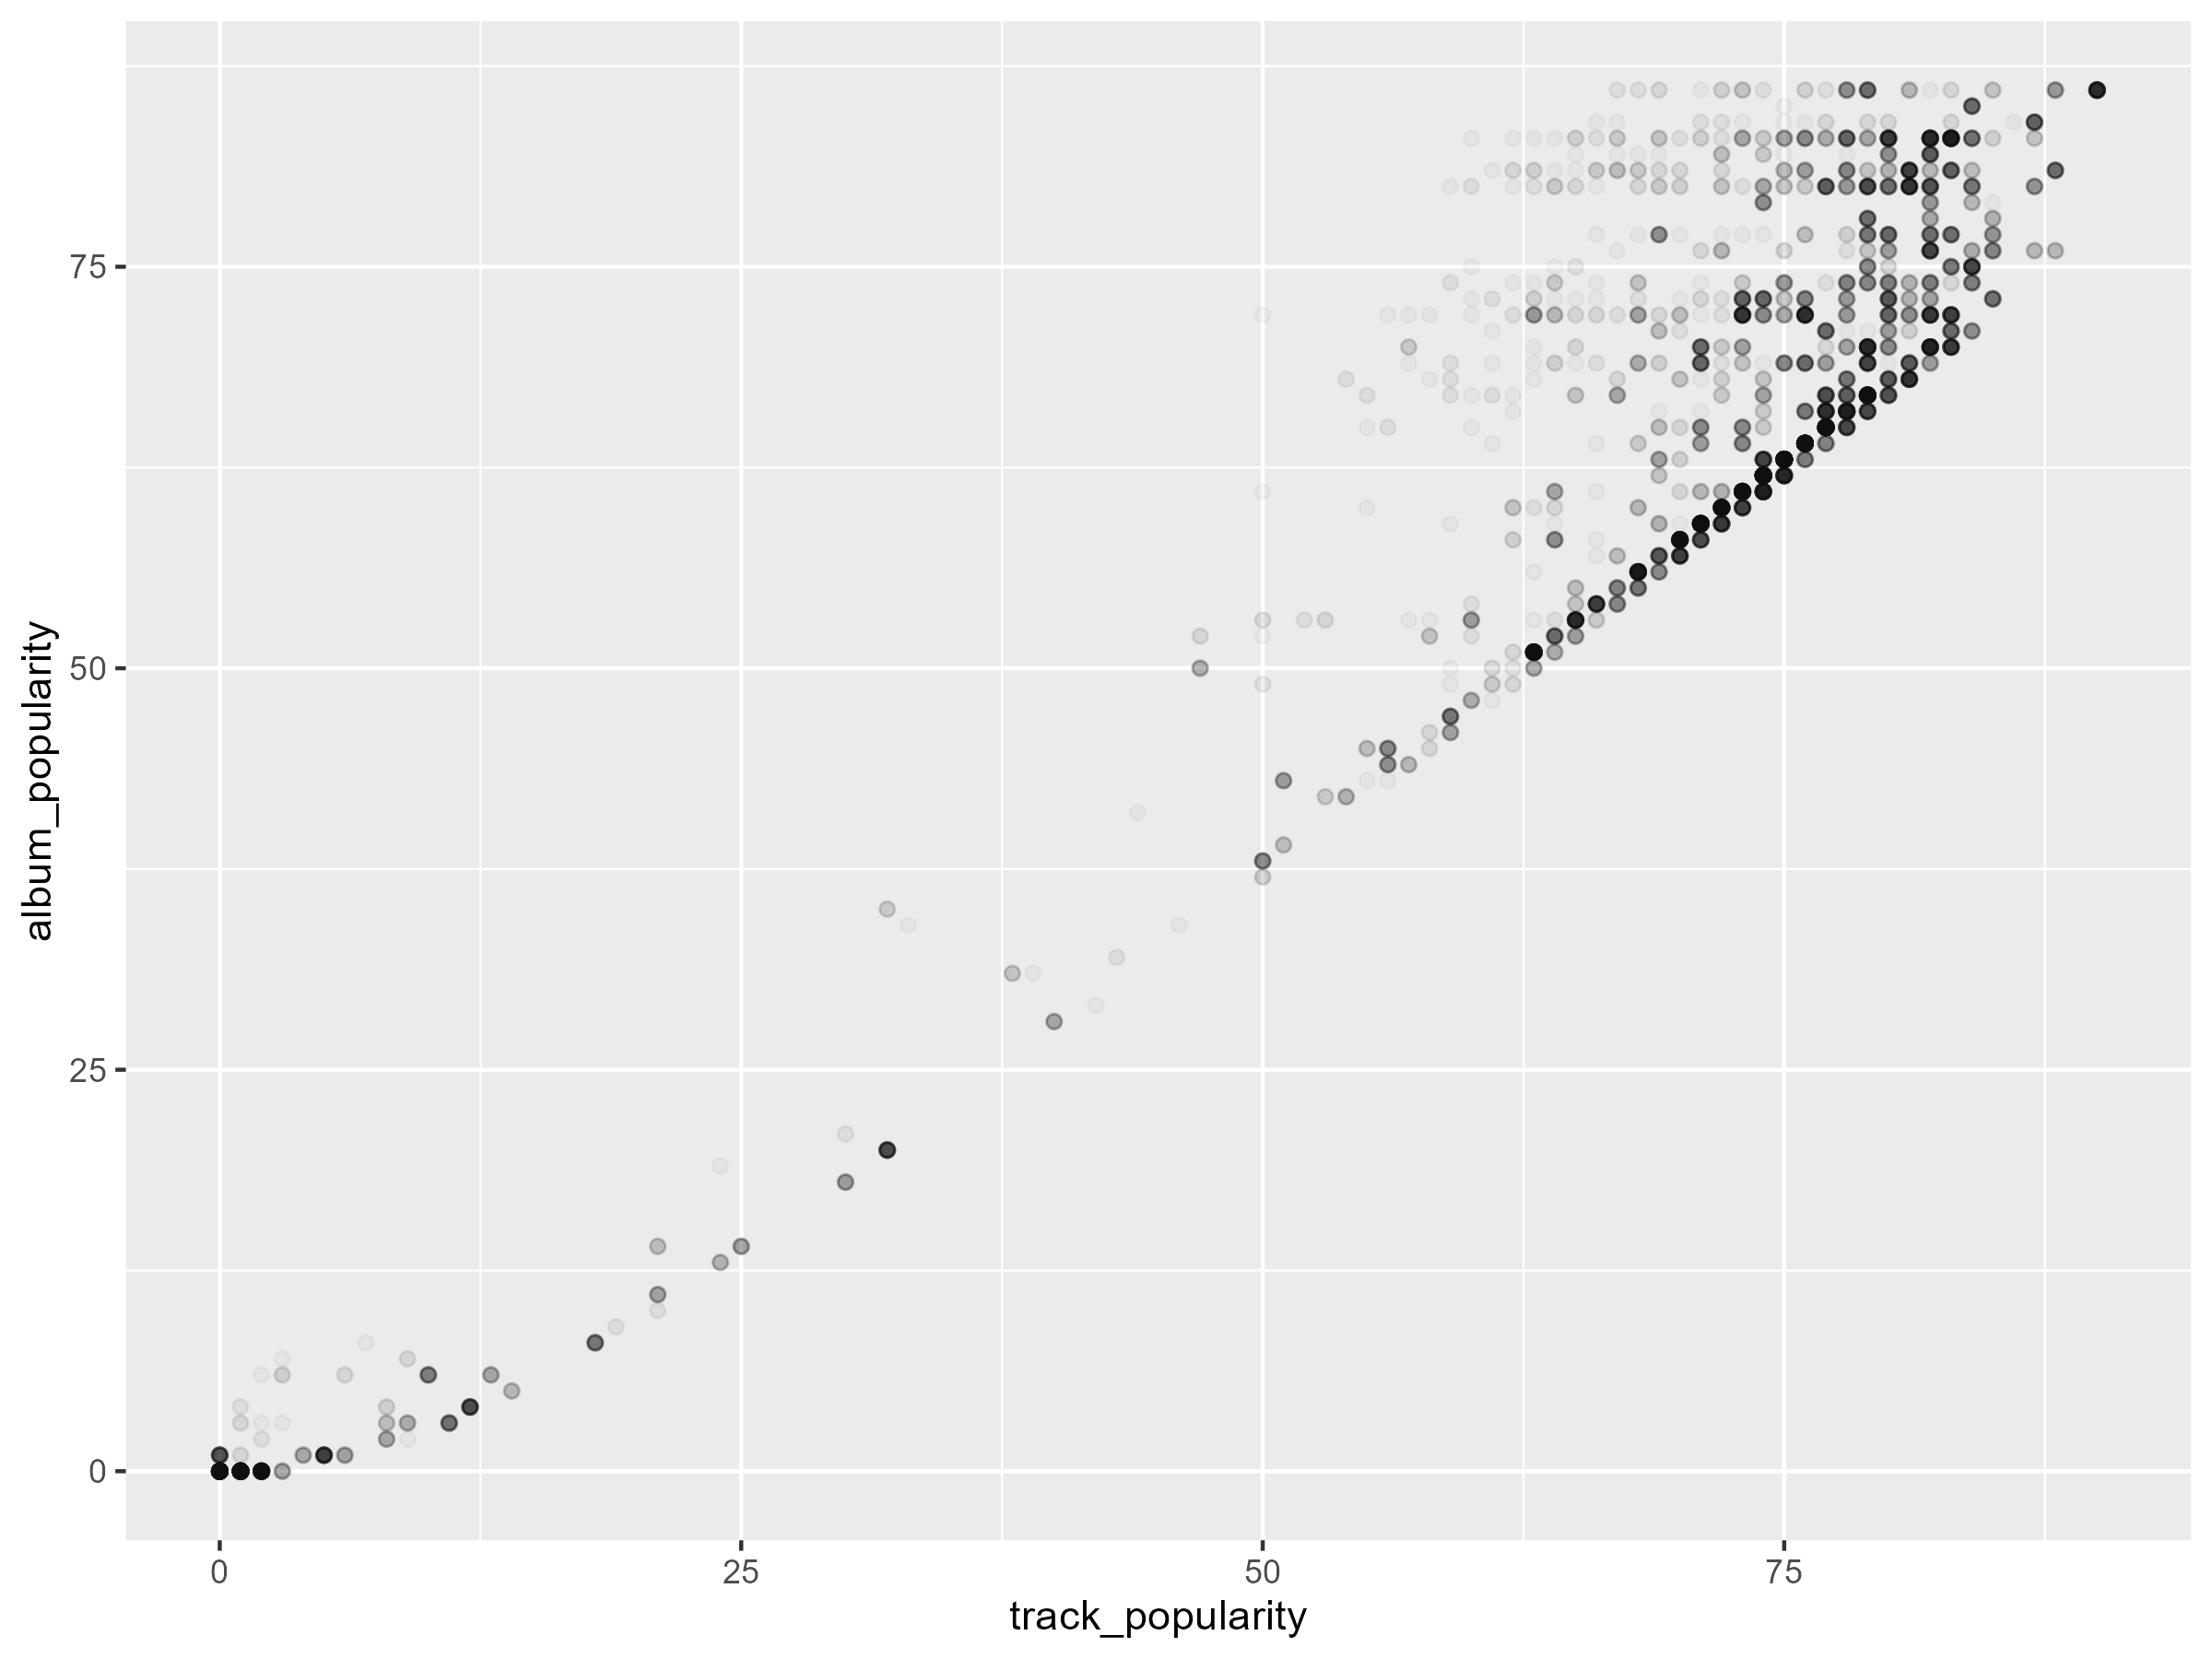
\includegraphics[width=0.8\textwidth]{Images/2_Bivariate/trackalbum.png}
    \caption{Scatter plot de \textit{Track popularity} amb \textit{Album popularity}}
    \label{fig:BivariateR_trackalbum}
\end{figure}

D’aquest anàlisi es poden extreure algunes conclusions interessants. D'entrada, es comentarà la combinació d'una variable categòrica amb una numèrica. Sembla ser que les cançons amb més popularitat provenen d’àlbums, enlloc de singles (\ref{fig:BivariateR_typepop}). Observem com les cançons pop són menys parlades que la resta (\ref{fig:BivariateR_speechpop}), al contrari que les de hip hop (que són bastant més parlades, una mitjana de 0.09 versus una de 0.15, \ref{fig:BivariateR_speechhip}). A més, les cançons d'aquest gènere són menys acústiques i més ballables i vives (\ref{fig:BivariateR_hipacoustic}). Les del gènere latino tenen un valence (positivitat) més elevada (\ref{fig:BivariateR_latinoval}).

\begin{figure}[H]
    \centering
    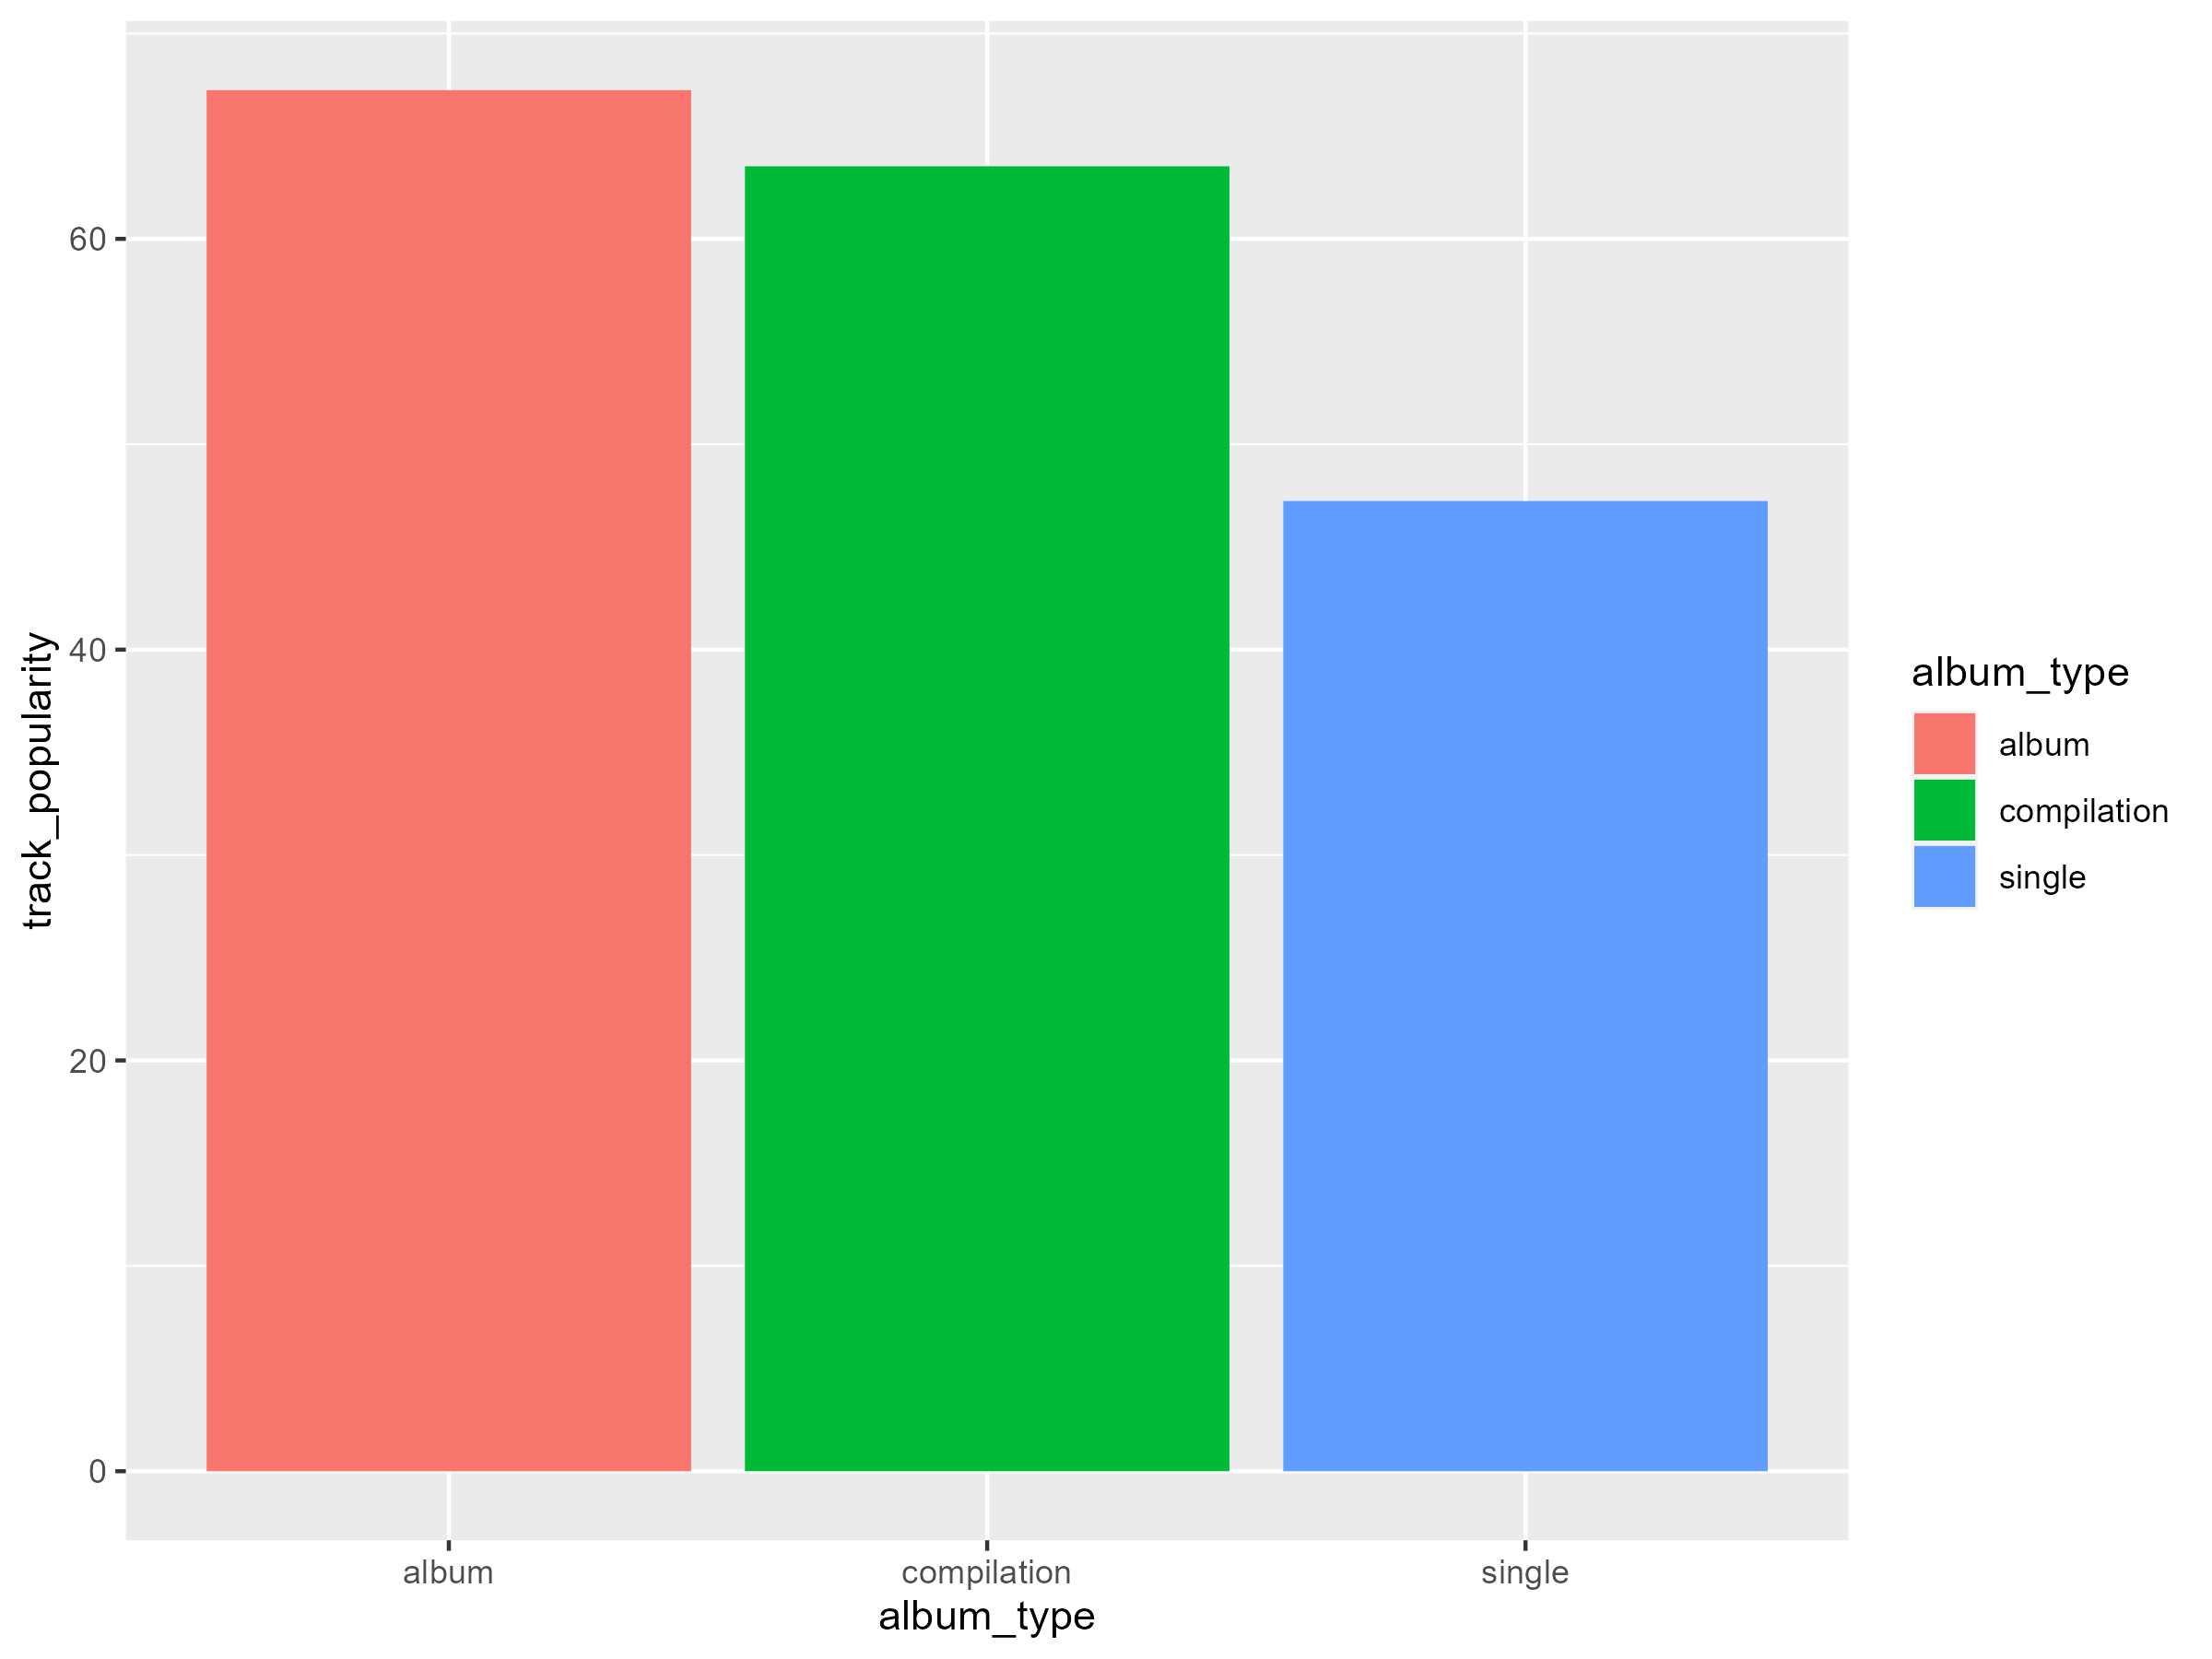
\includegraphics[width=0.8\textwidth]{Images/2_Bivariate/typepopularity.png}
    \caption{Bar plot \textit{album type} amb \textit{track popularity}}
    \label{fig:BivariateR_typepop}
\end{figure}

\begin{figure}[H]
\centering
    \begin{minipage}{.4\textwidth}
        \centering
        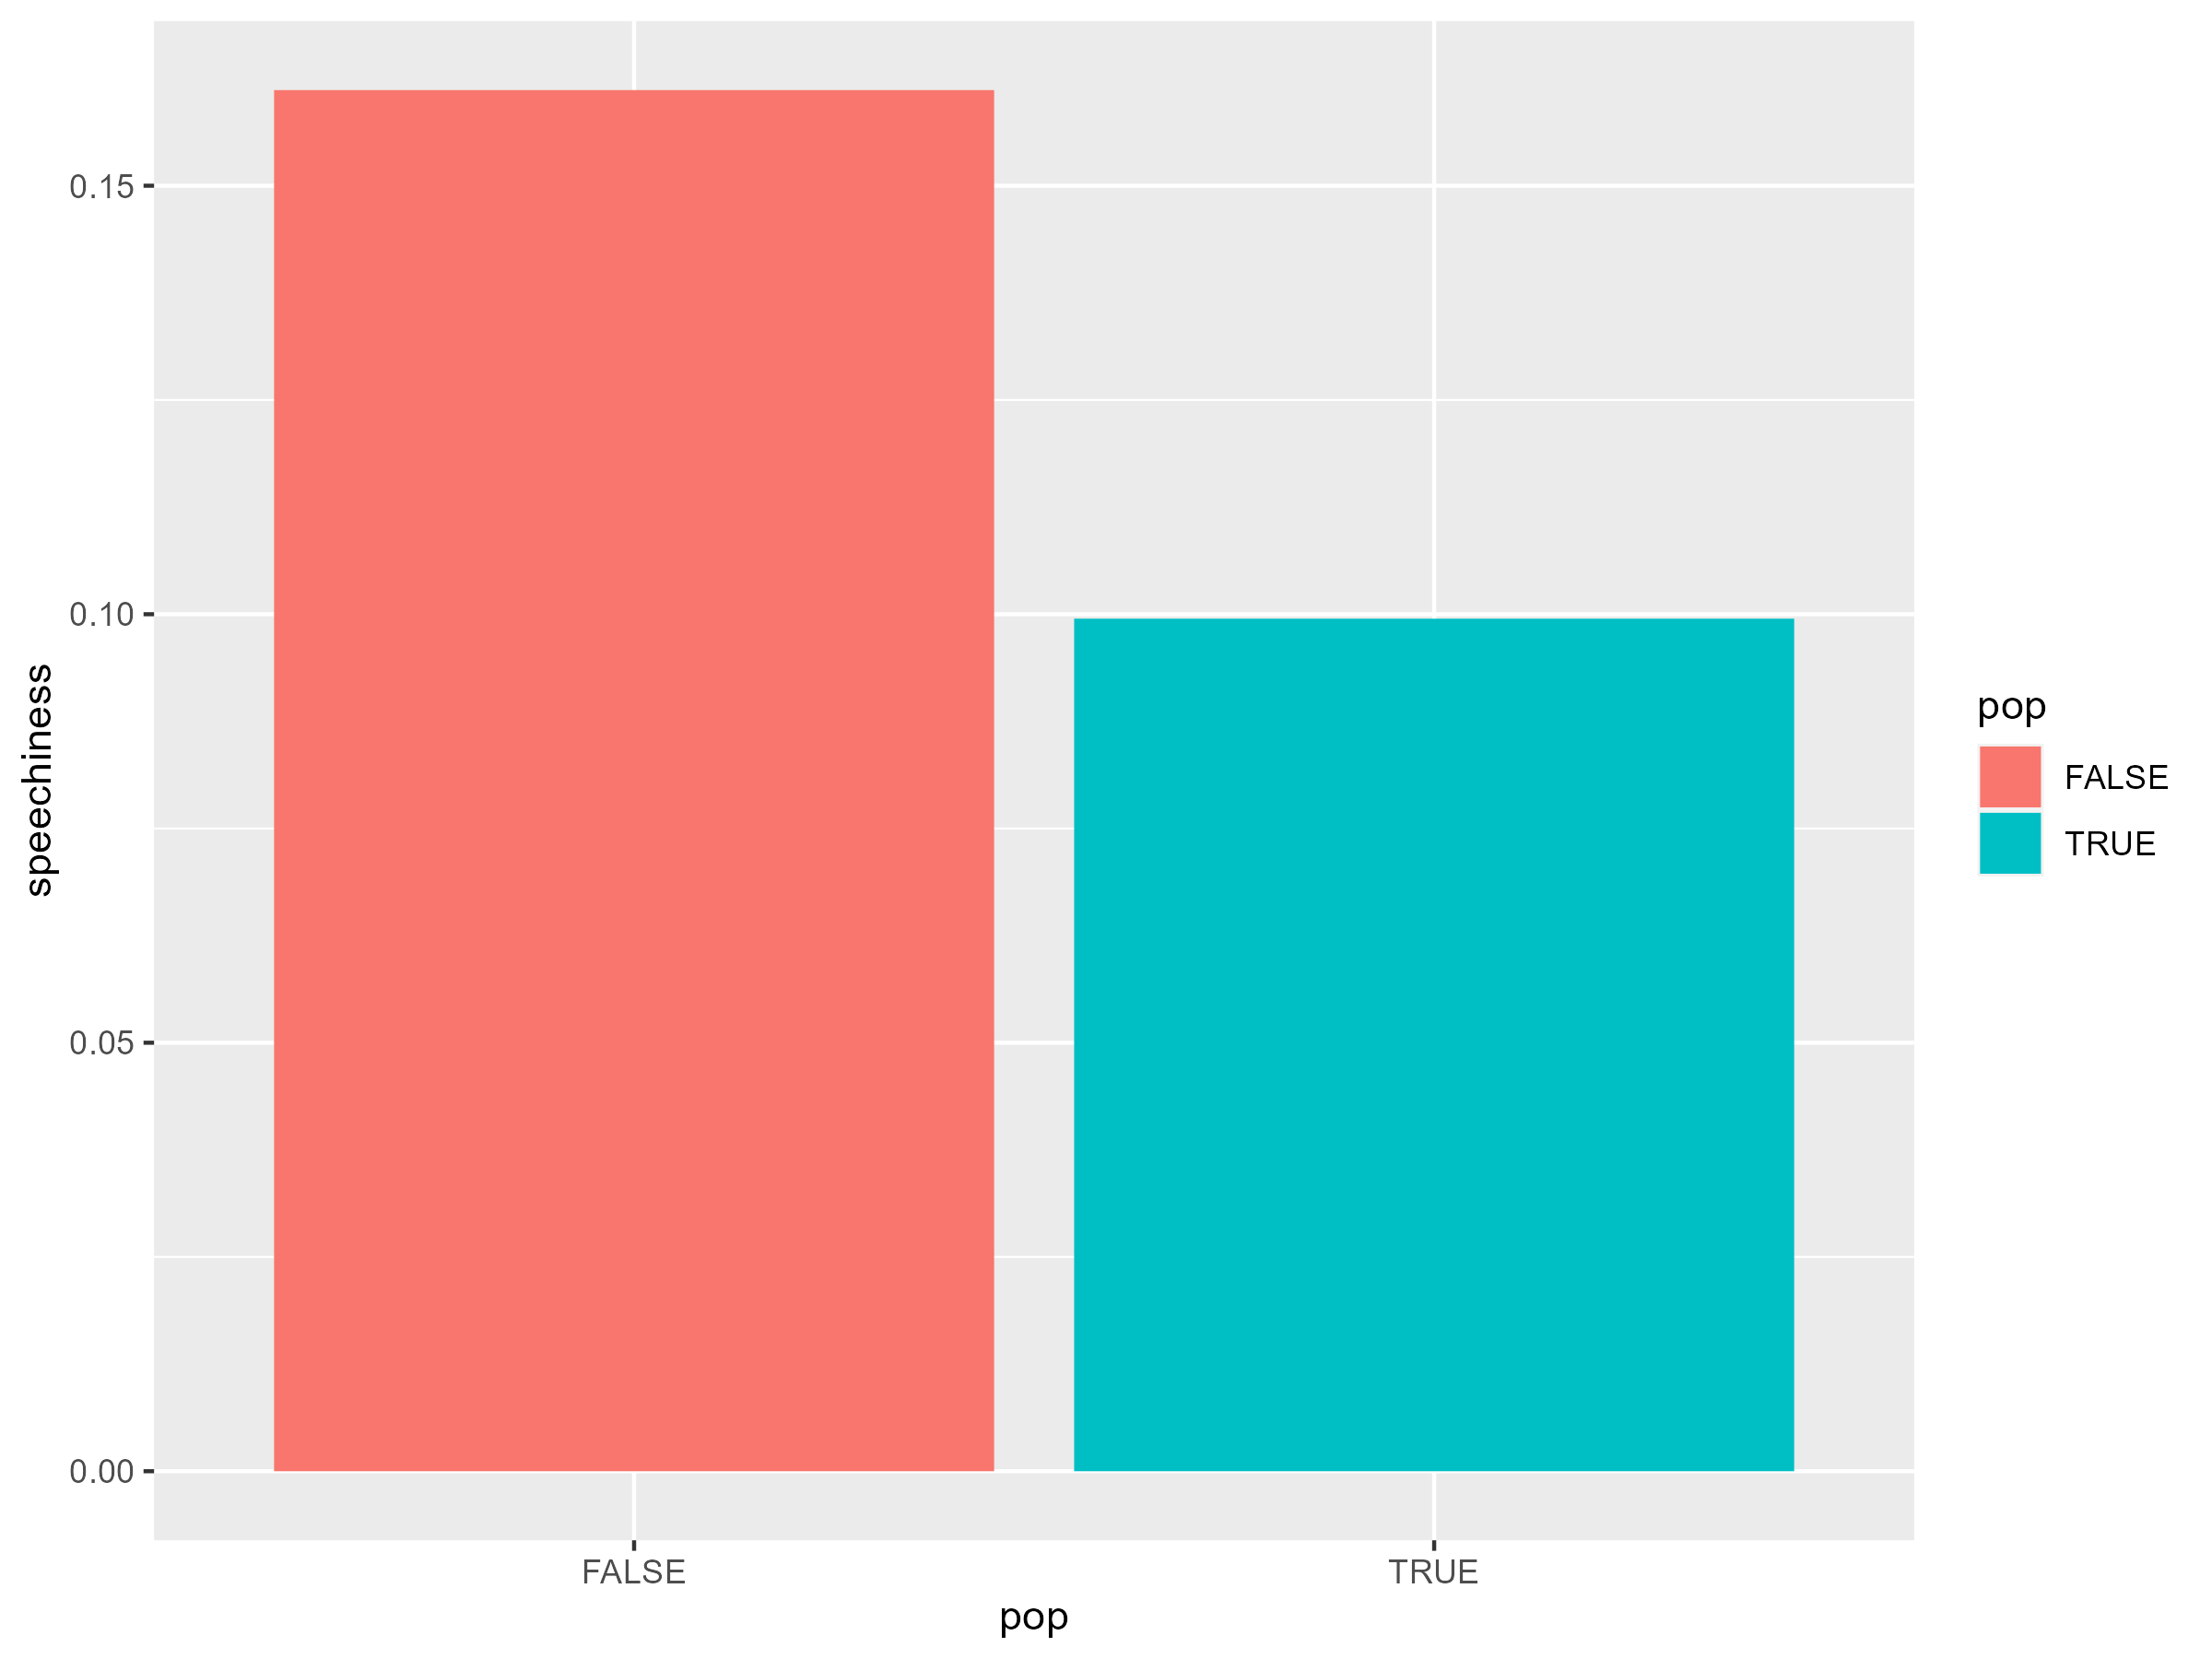
\includegraphics[width=0.95\linewidth]{Images/2_Bivariate/popspeech.png}
        \caption{Bar plot \textit{pop} amb \textit{speechiness}}
        \label{fig:BivariateR_speechpop}
    \end{minipage}%
    \begin{minipage}{.4\textwidth}
        \centering
        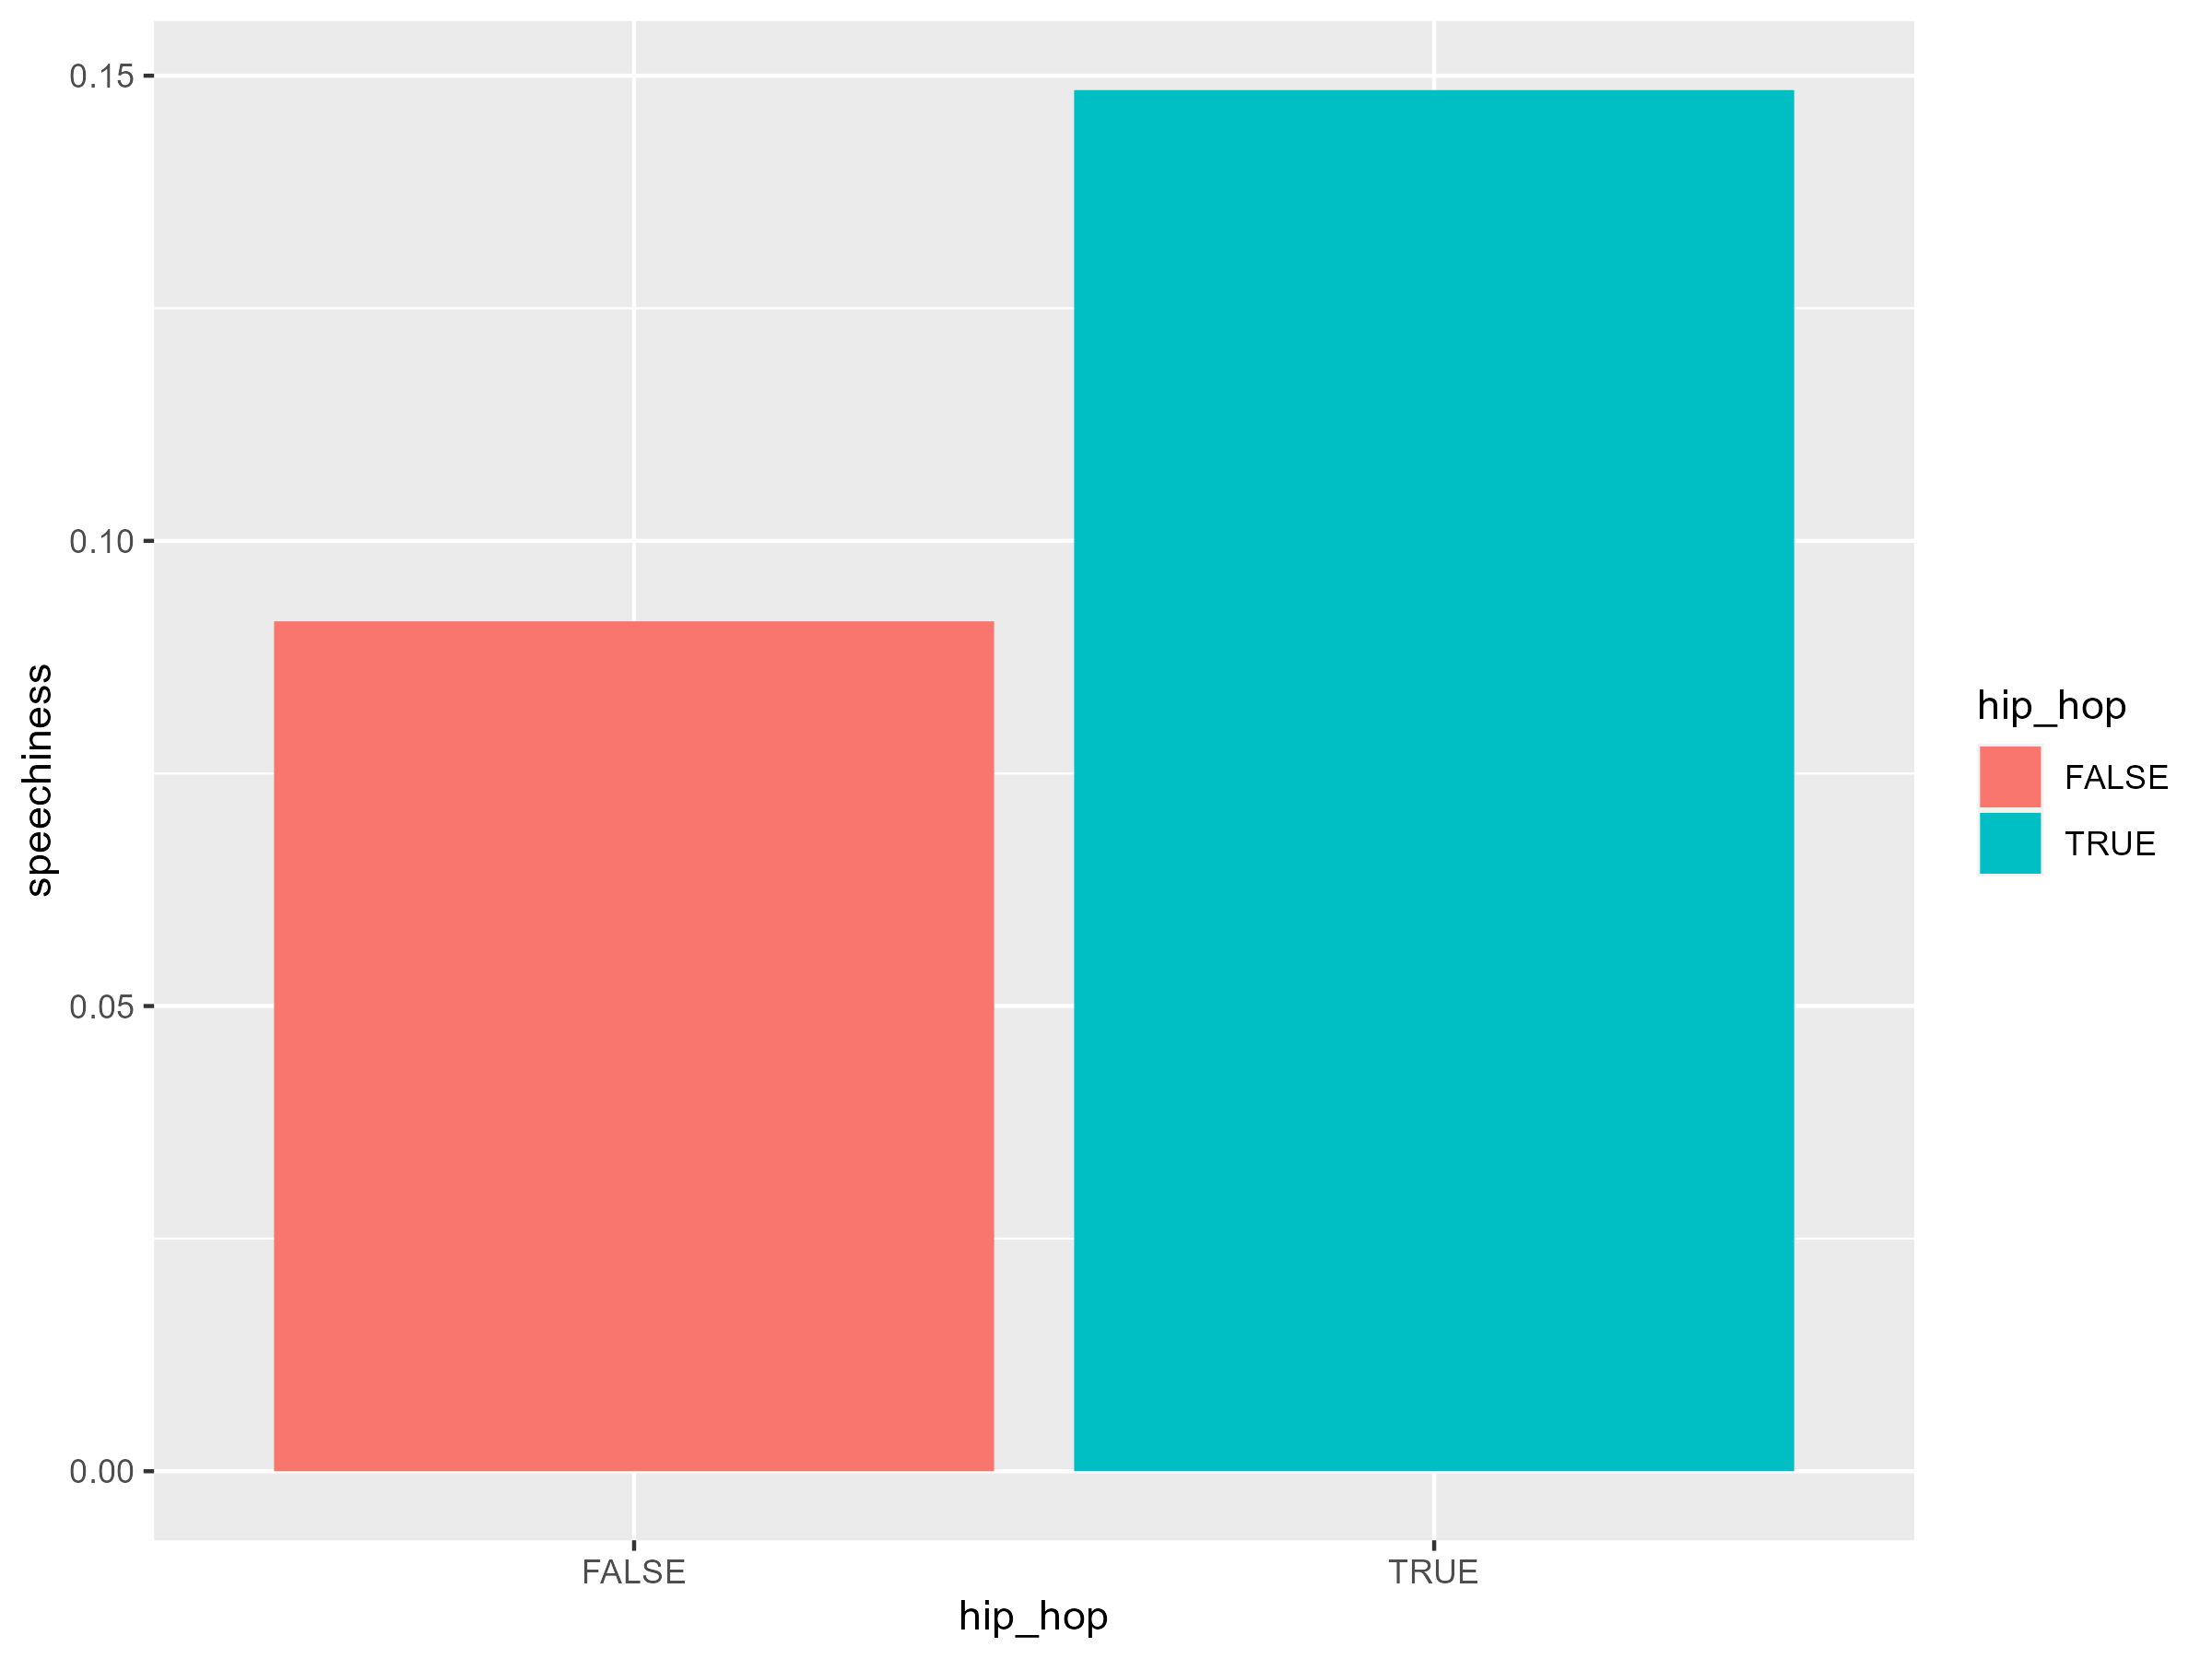
\includegraphics[width=0.95\linewidth]{Images/2_Bivariate/hiphopspeech.png}
        \caption{Bar plot \textit{hip hop} amb \textit{speechiness}}
        \label{fig:BivariateR_speechhip}
    \end{minipage}%
\end{figure}

\begin{figure}[H]
\centering
    \begin{minipage}{.4\textwidth}
        \centering
        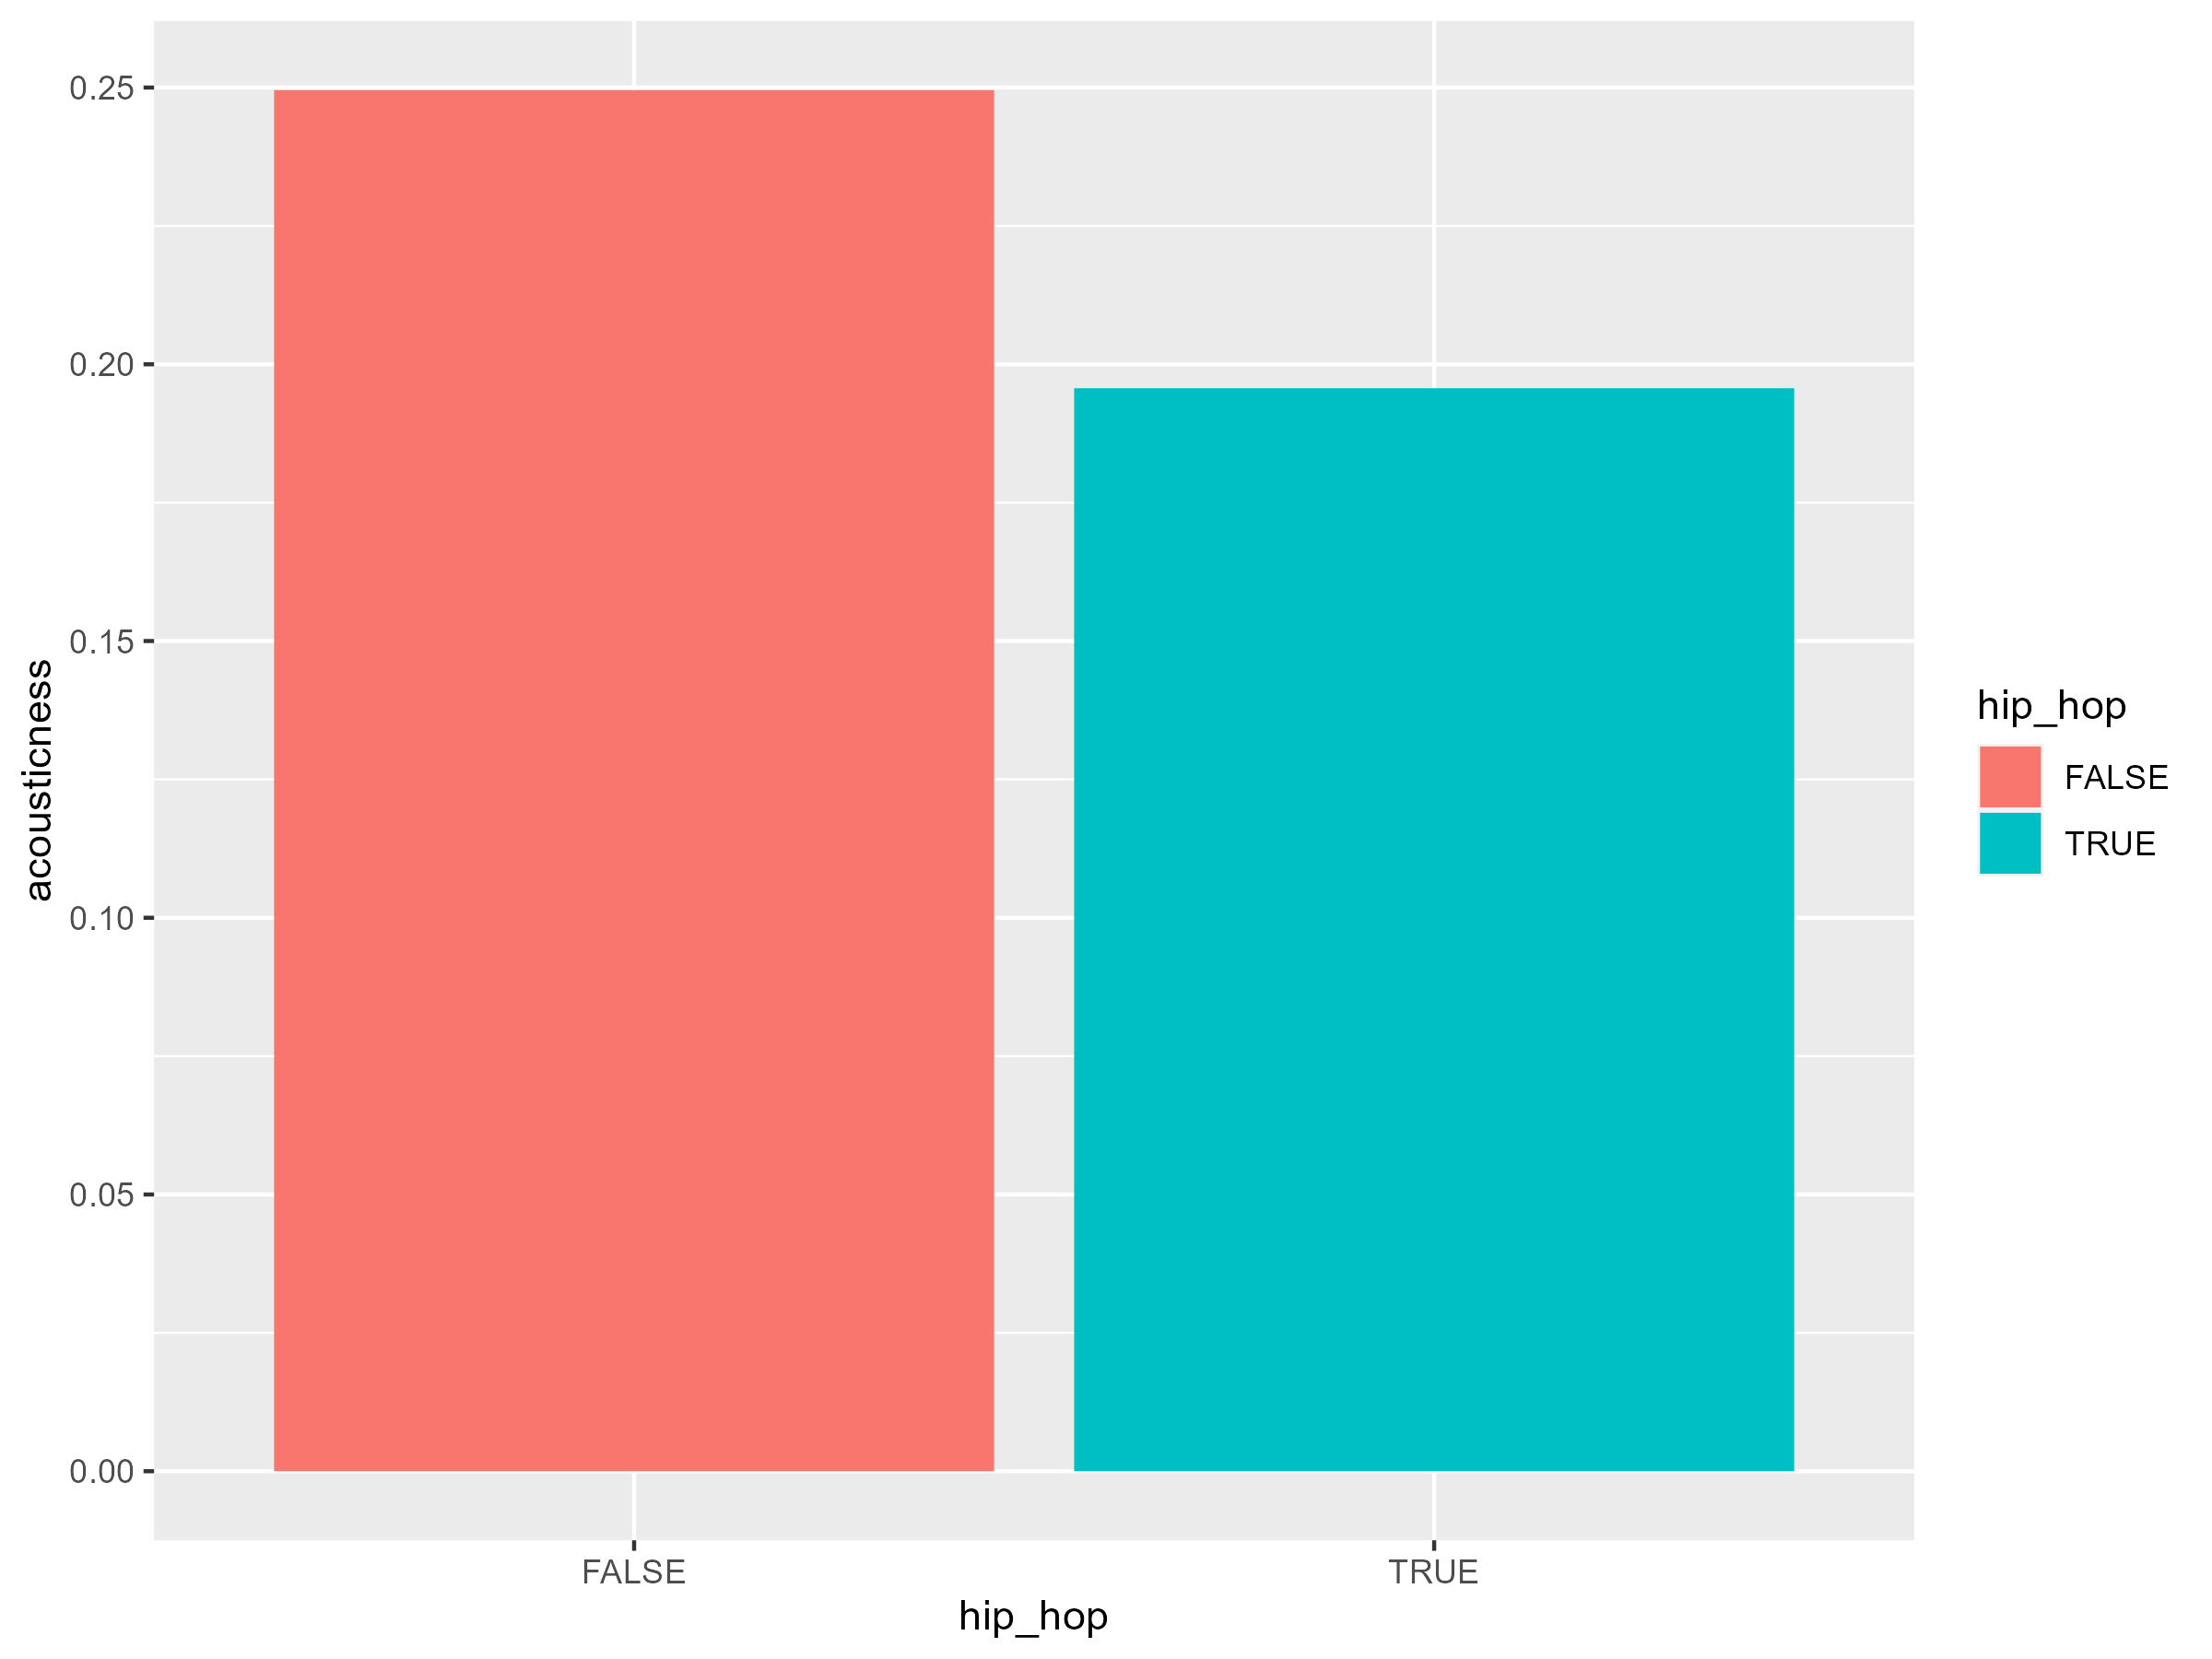
\includegraphics[width=0.95\linewidth]{Images/2_Bivariate/hiphopacoustic.png}
        \caption{Bar plot \textit{hip hop} amb \textit{acousticness}}
        \label{fig:BivariateR_hipacoustic}
    \end{minipage}%
    \begin{minipage}{.4\textwidth}
        \centering
        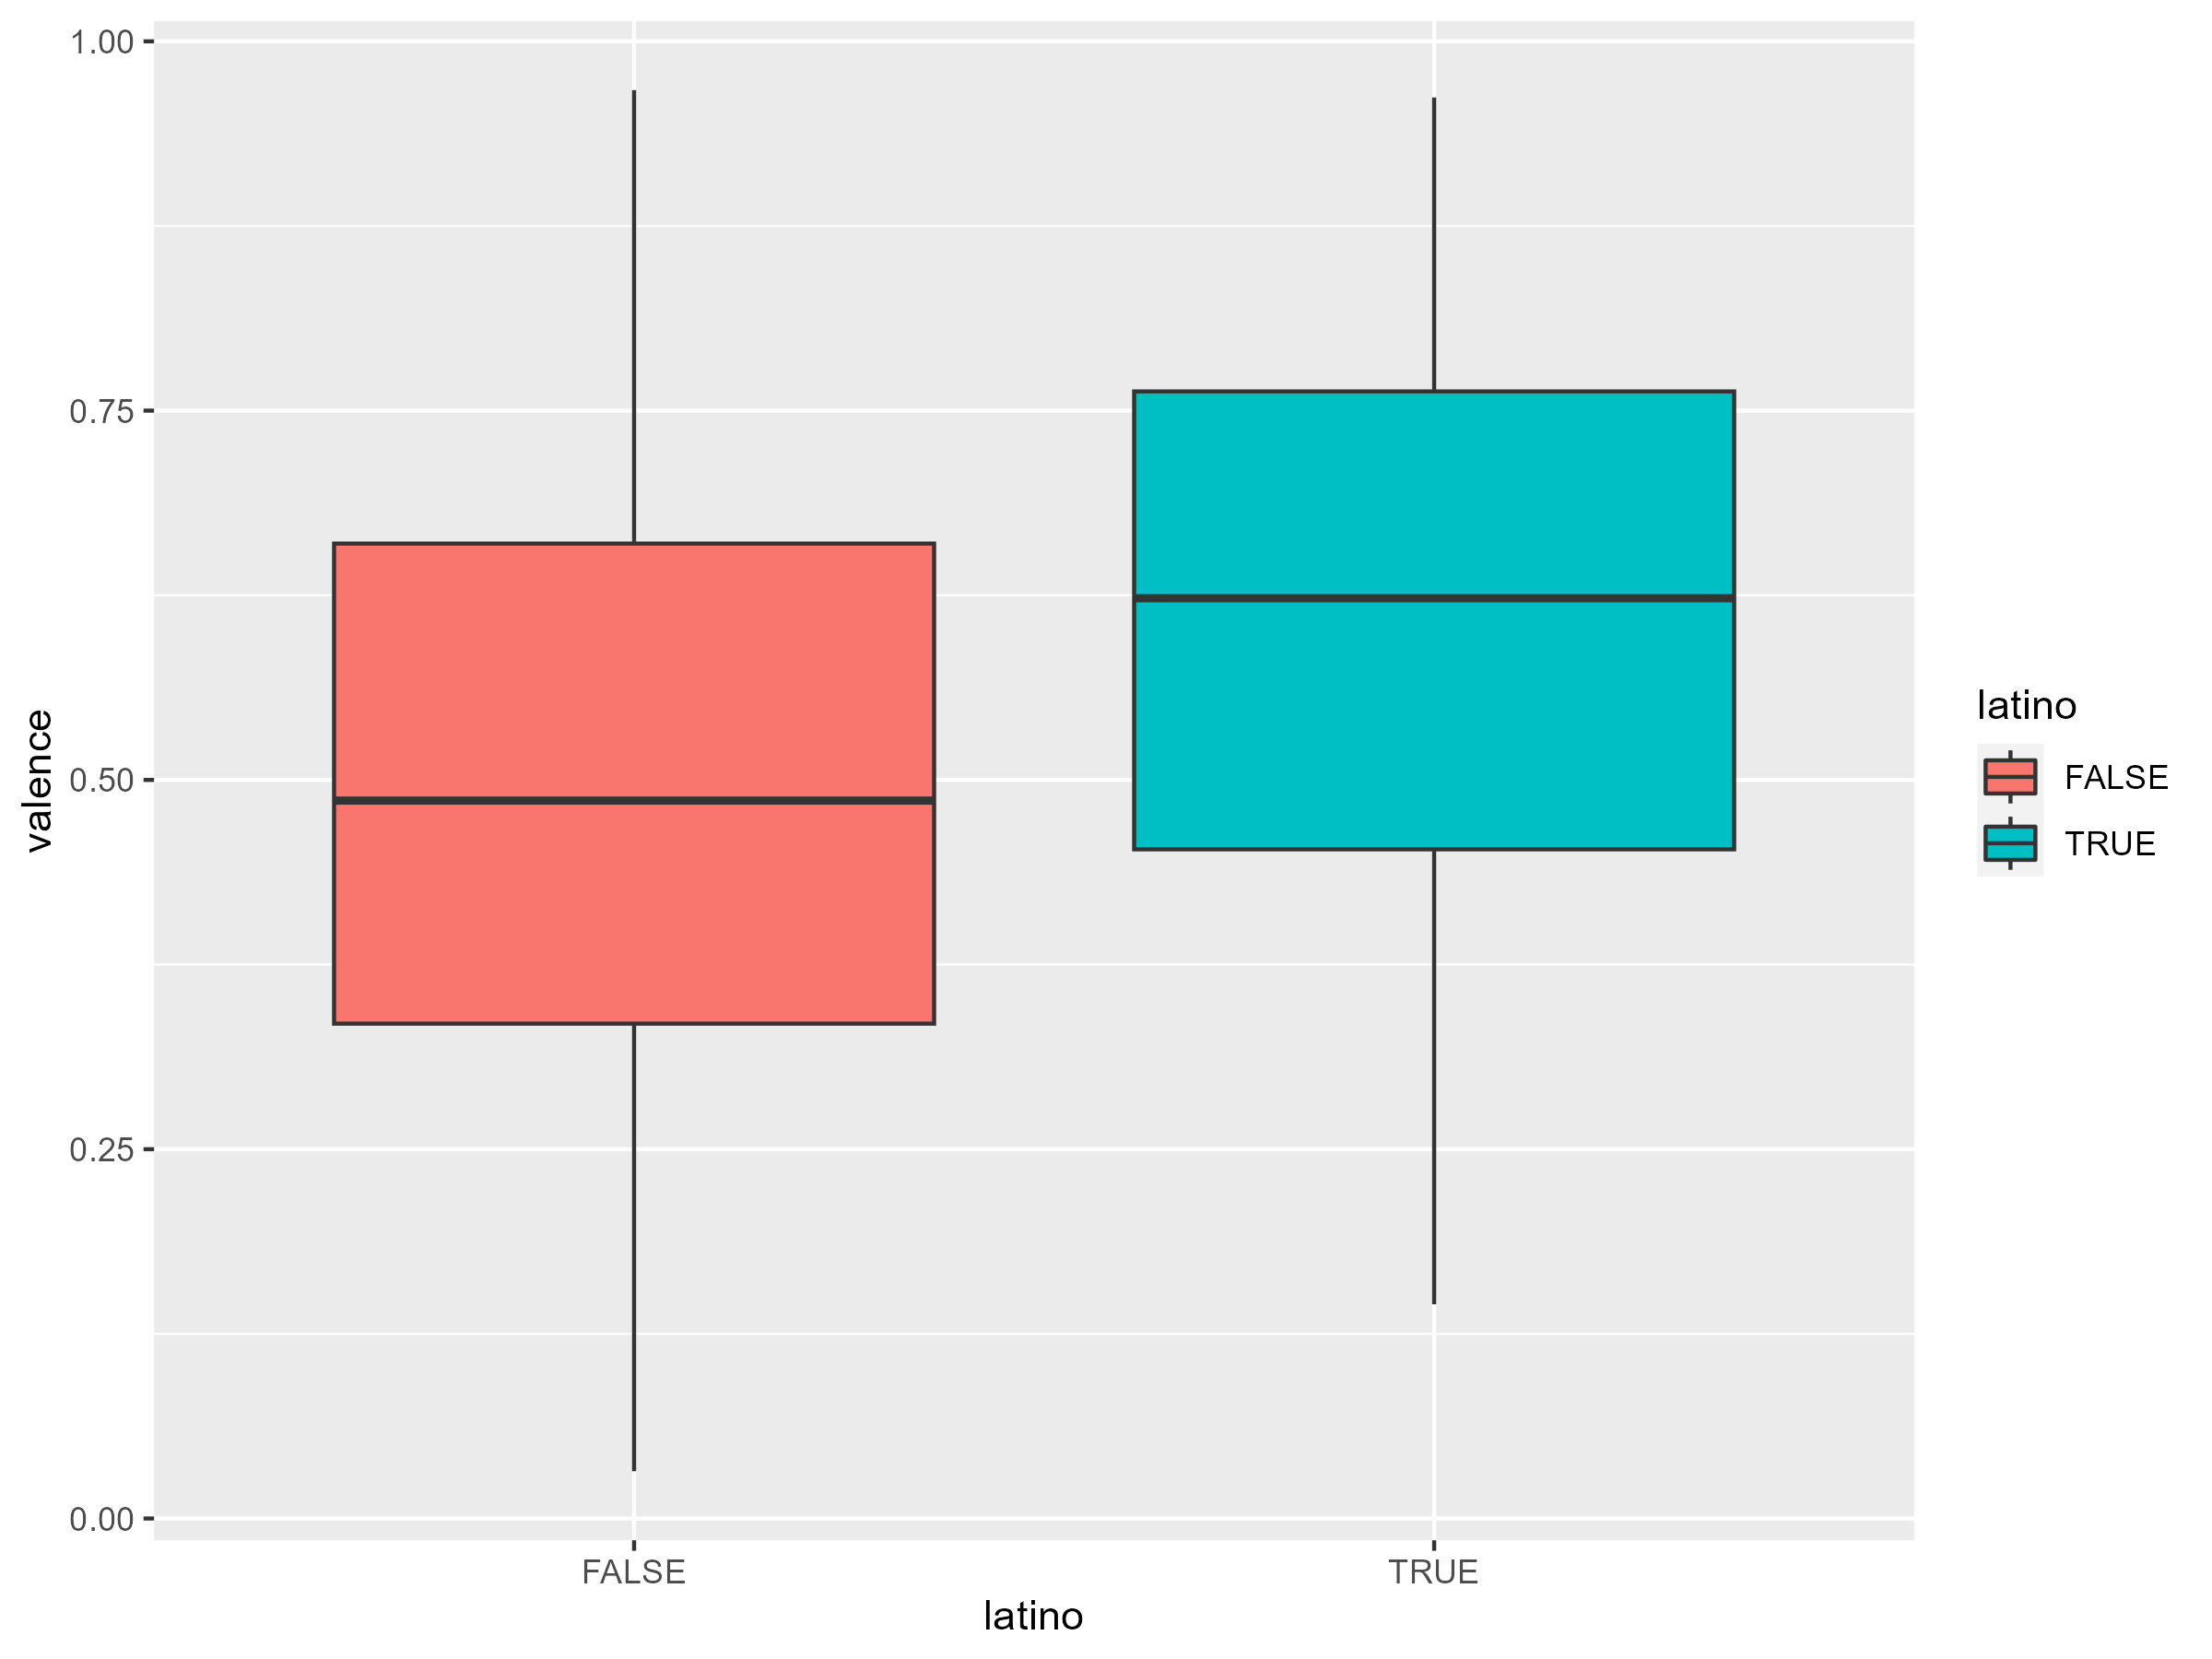
\includegraphics[width=0.95\linewidth]{Images/2_Bivariate/latinovalence.png}
        \caption{Box plots \textit{latino} amb \textit{valence}}
        \label{fig:BivariateR_latinoval}
    \end{minipage}%
\end{figure}


Altres resultats són més obvis, com que les cançons que no són colaboracions tenen només un artista (\ref{fig:BivariateR_collabnum}). Els grups de música tenen cançons menys parlades i també menys acústiques(\ref{fig:BivariateR_groupacustic}). Les artistes (gènere femení) tenen lleugerament més reproduccions (de mitjana) que els artistes (masculí), i alhora moltes més que els grups mixtos (\ref{fig:BivariateR_genderstreams}). A més, observant la comparació amb artist num, podem observar que el gènere female sol comptar amb la participació de menys artistes que el male (\ref{fig:BivariateR_gendernum}).

\begin{figure}[H]
\centering
    \begin{minipage}{.4\textwidth}
        \centering
        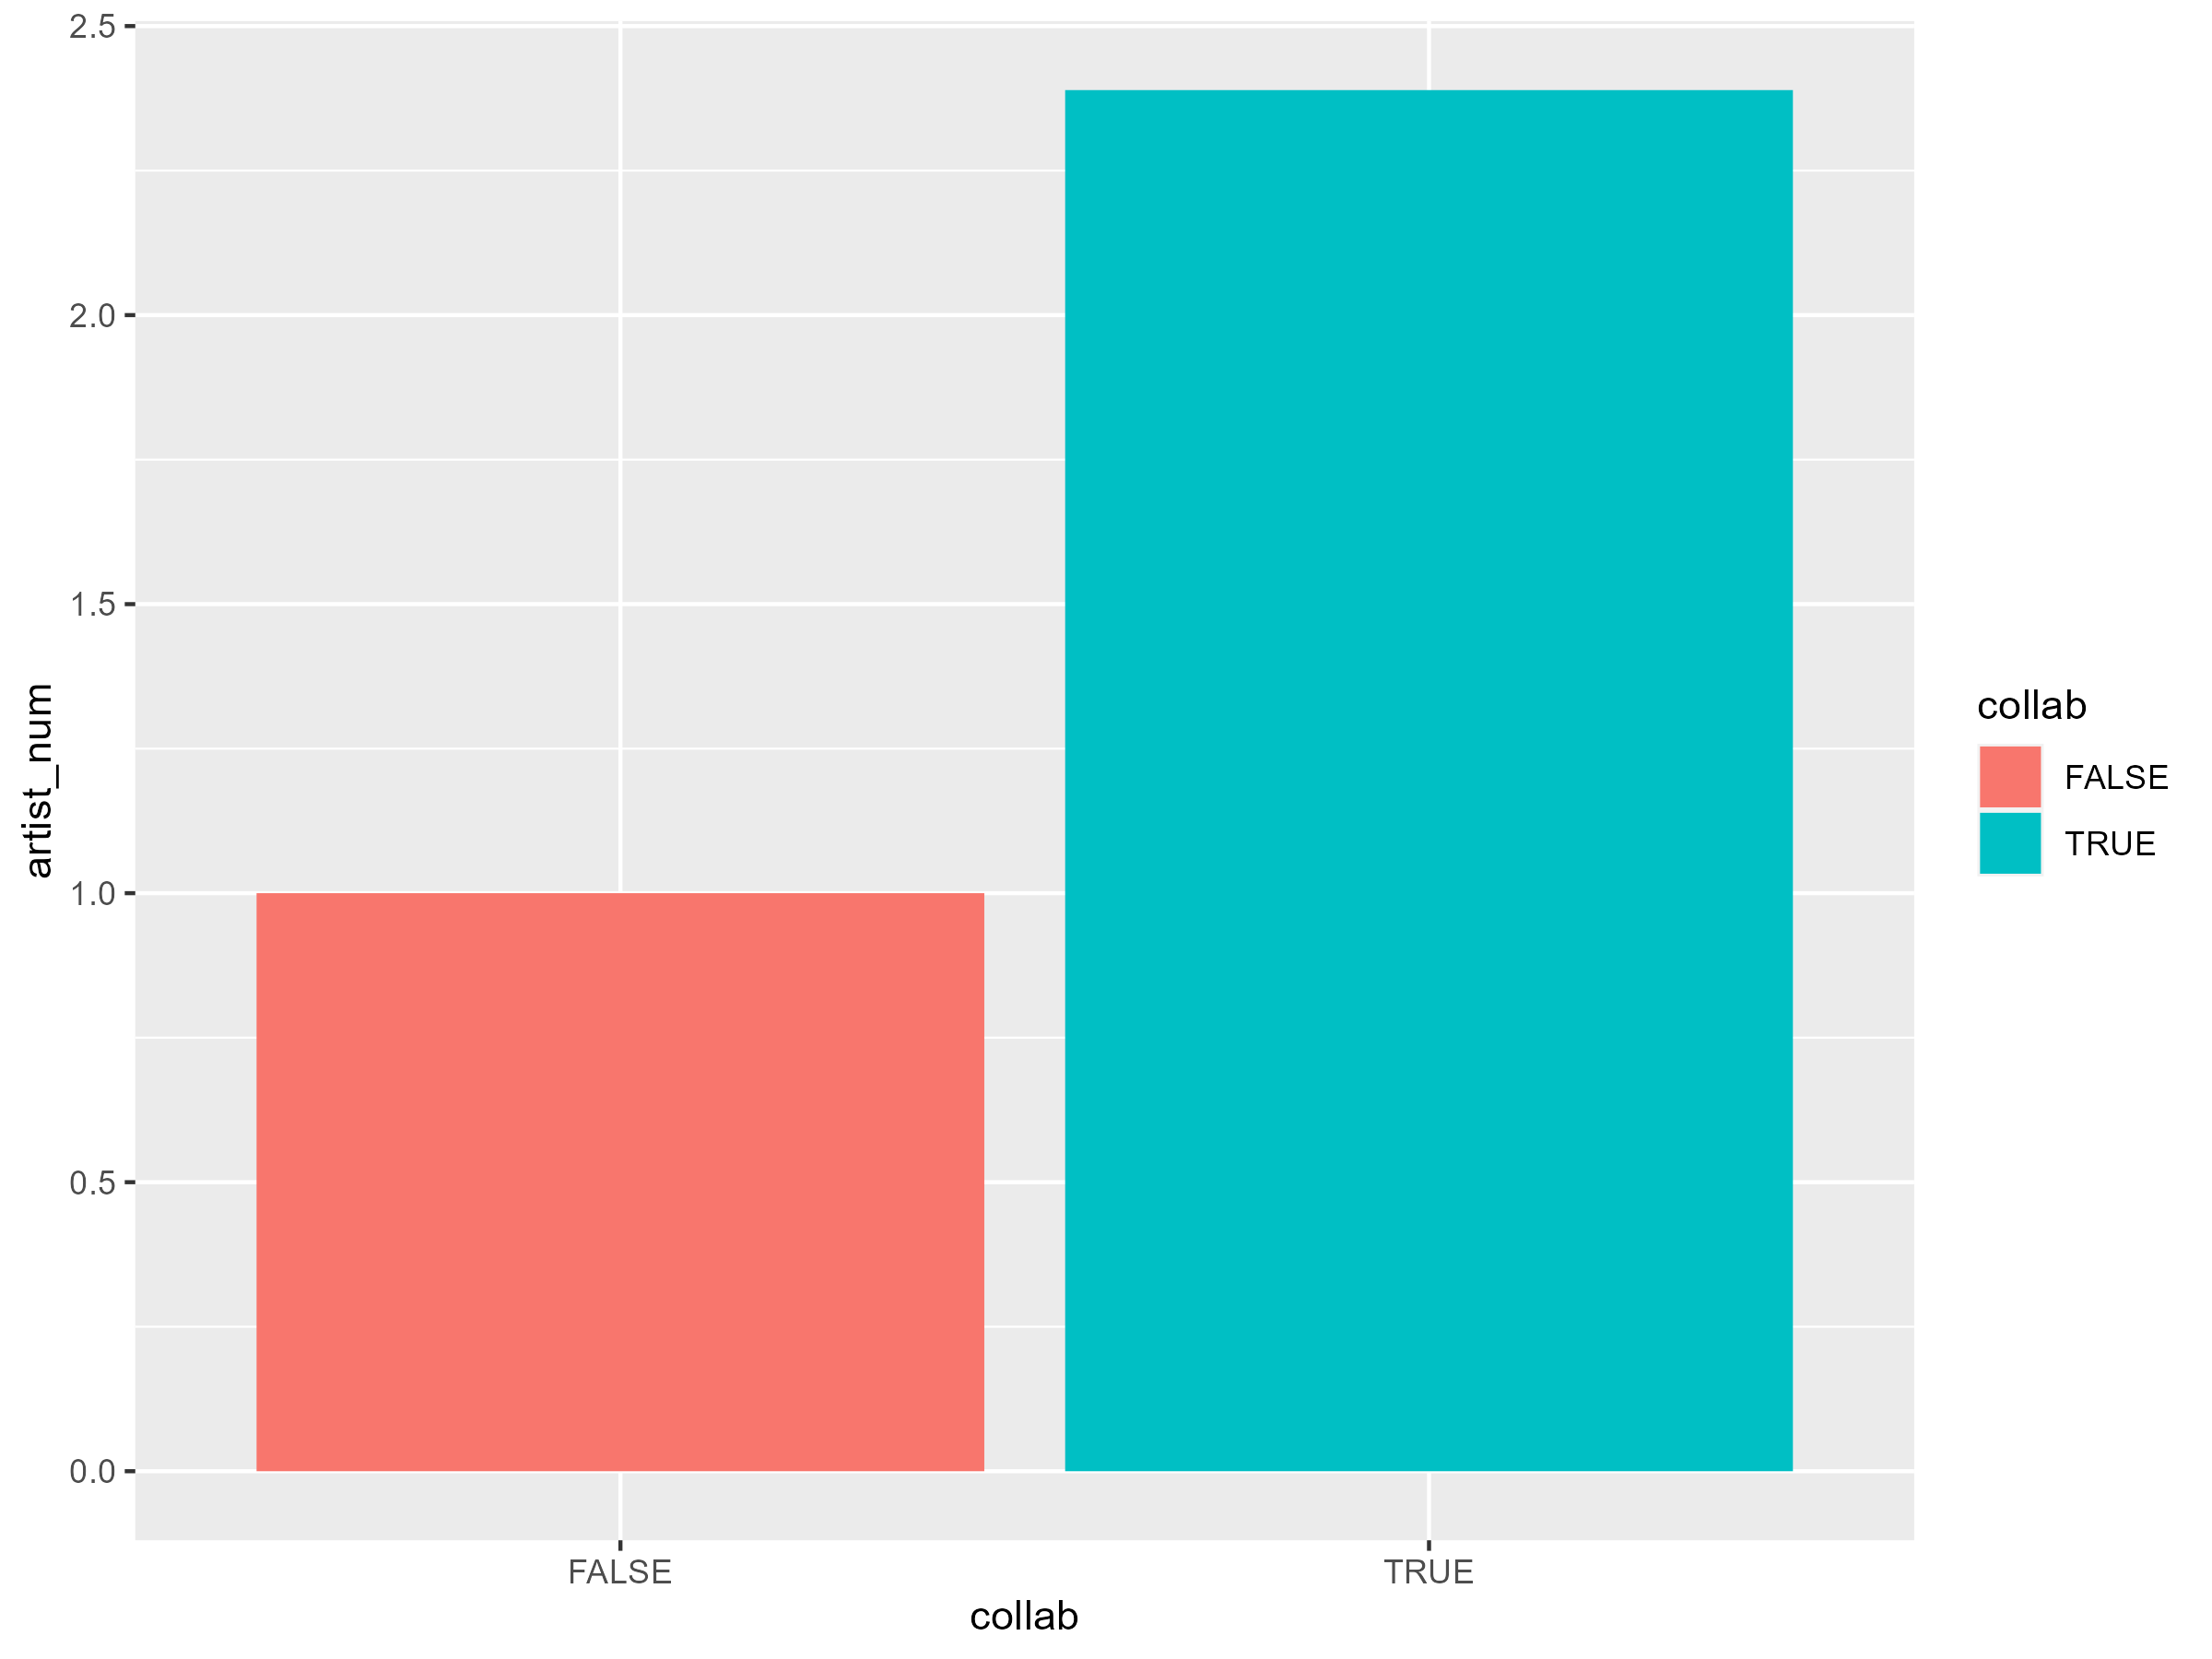
\includegraphics[width=0.95\linewidth]{Images/2_Bivariate/collabnum.png}
        \caption{Bar plot \textit{collab} amb \textit{artist num}}
        \label{fig:BivariateR_collabnum}
    \end{minipage}%
    \begin{minipage}{.4\textwidth}
        \centering
        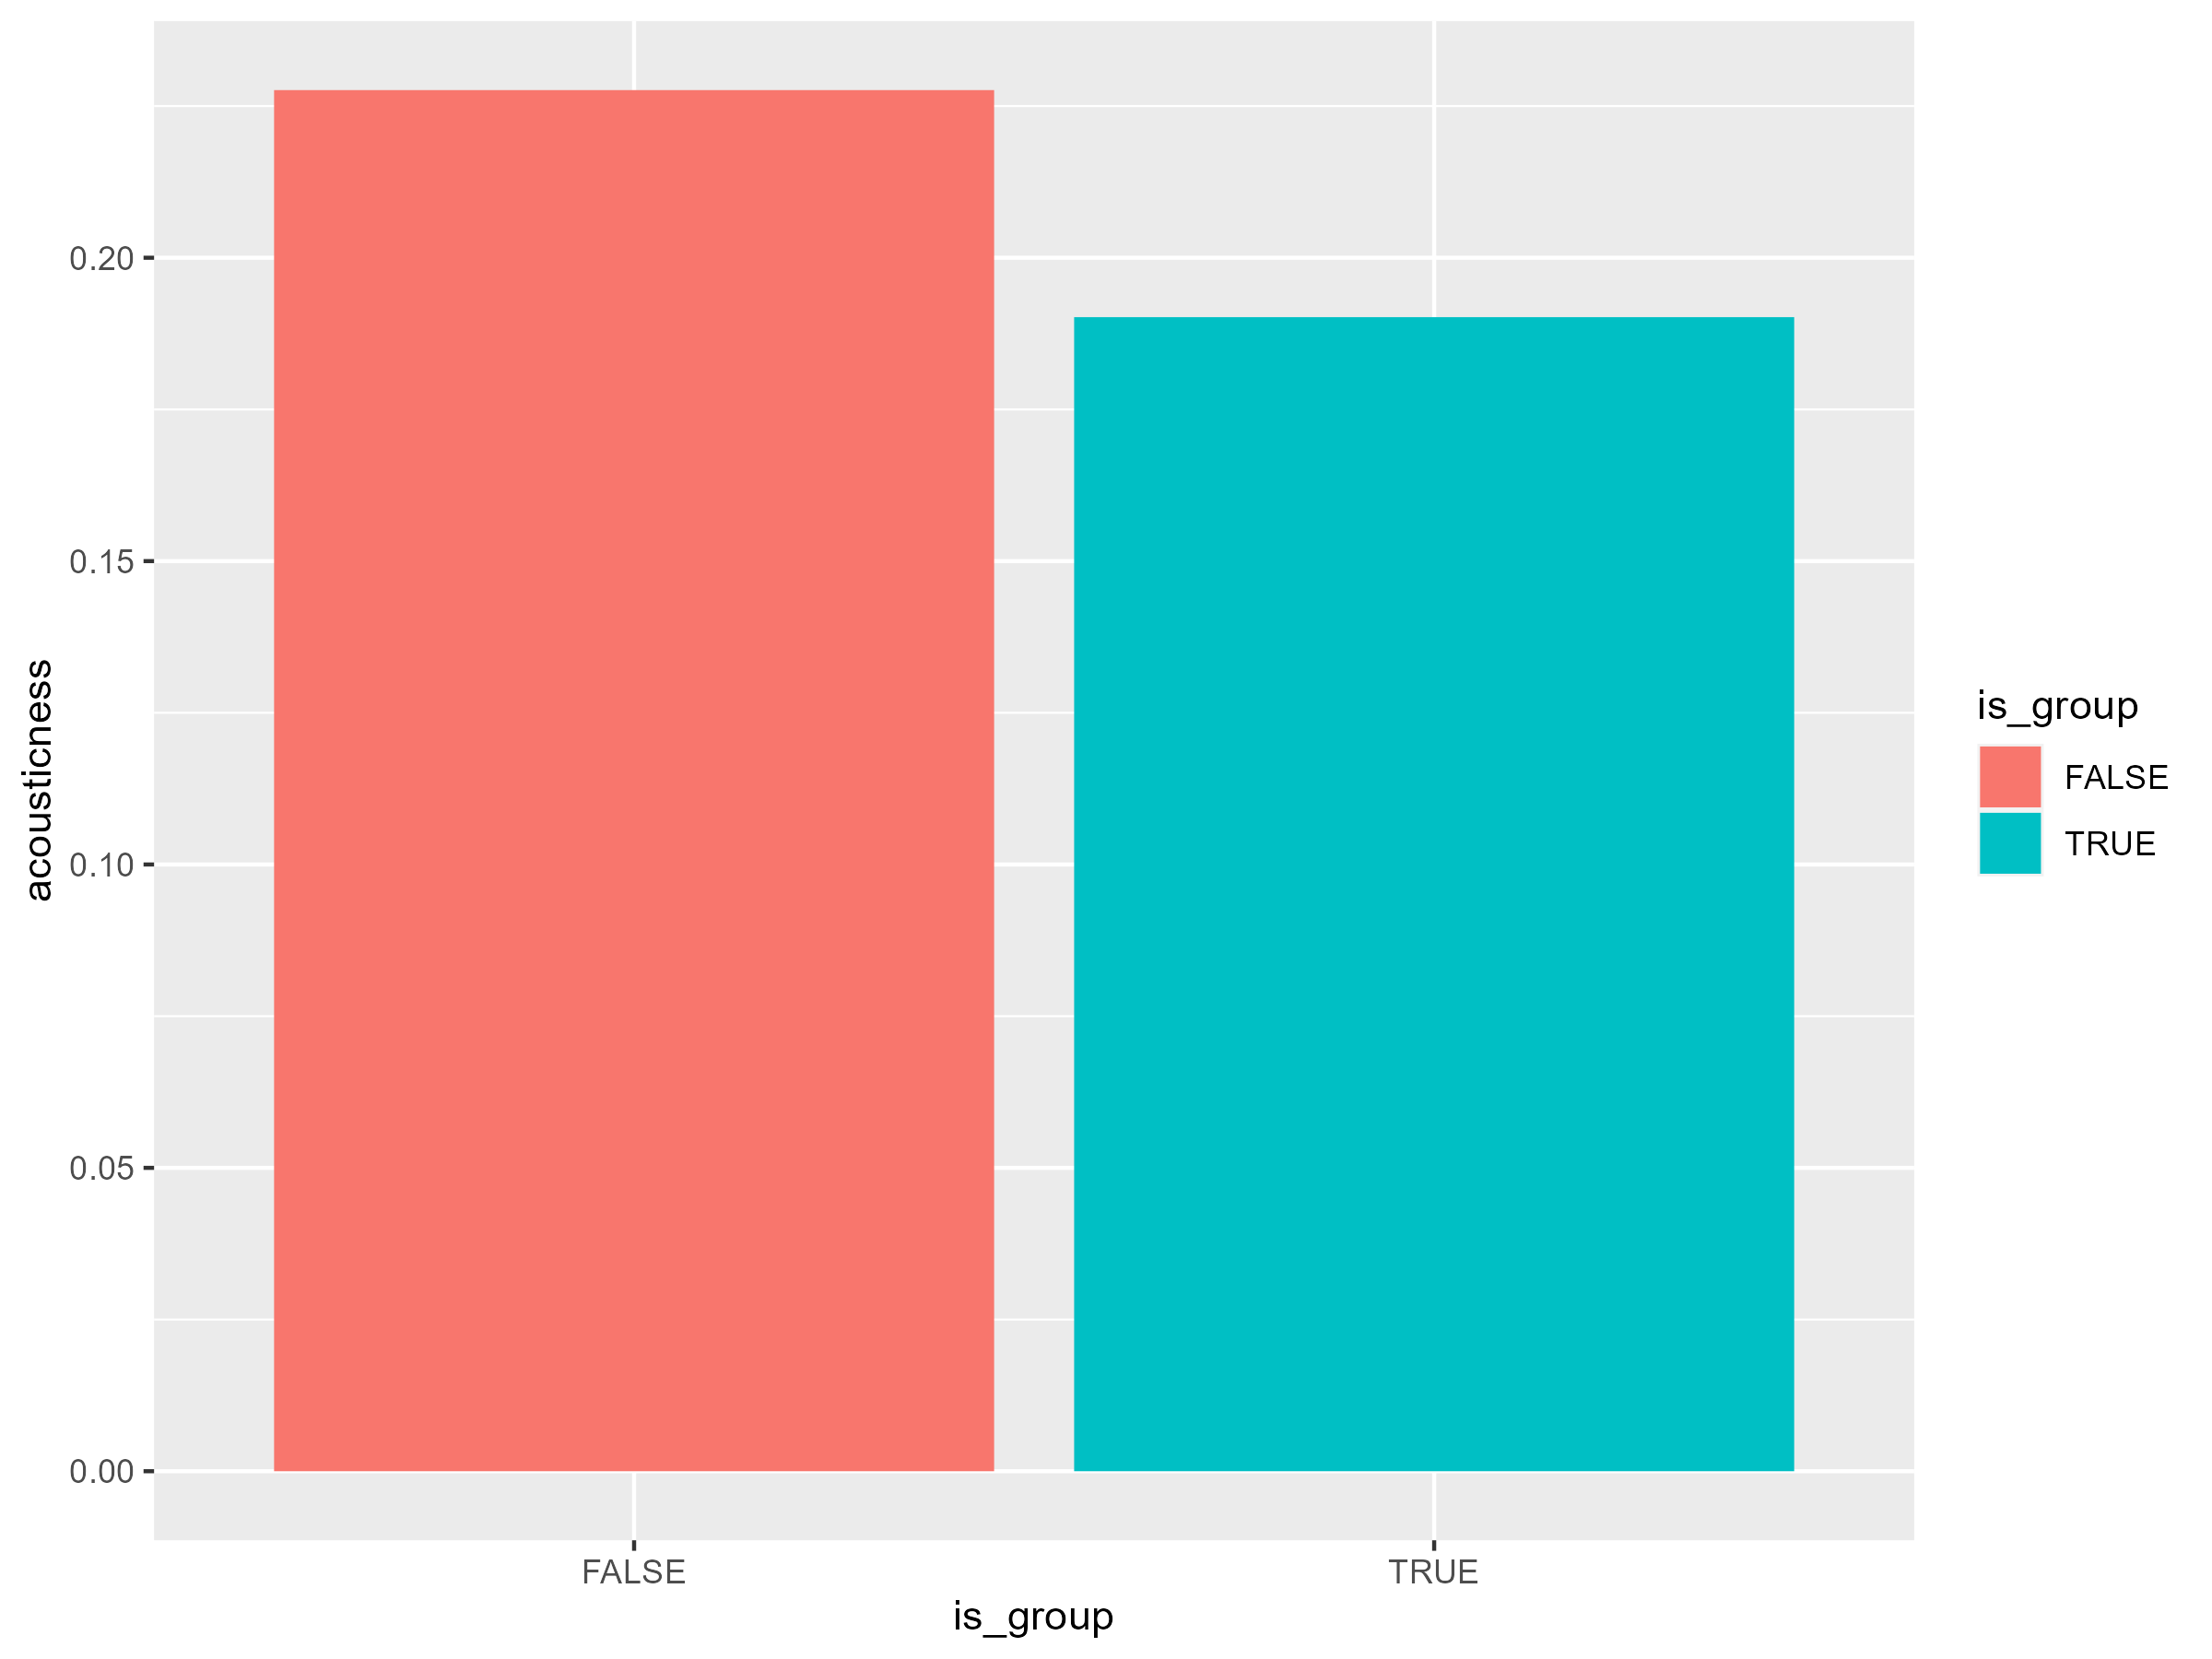
\includegraphics[width=0.95\linewidth]{Images/2_Bivariate/groupacoustic.png}
        \caption{Bar plot \textit{group} amb \textit{acousticness}}
        \label{fig:BivariateR_groupacustic}
    \end{minipage}%
\end{figure}

\begin{figure}[H]
\centering
    \begin{minipage}{.4\textwidth}
        \centering
        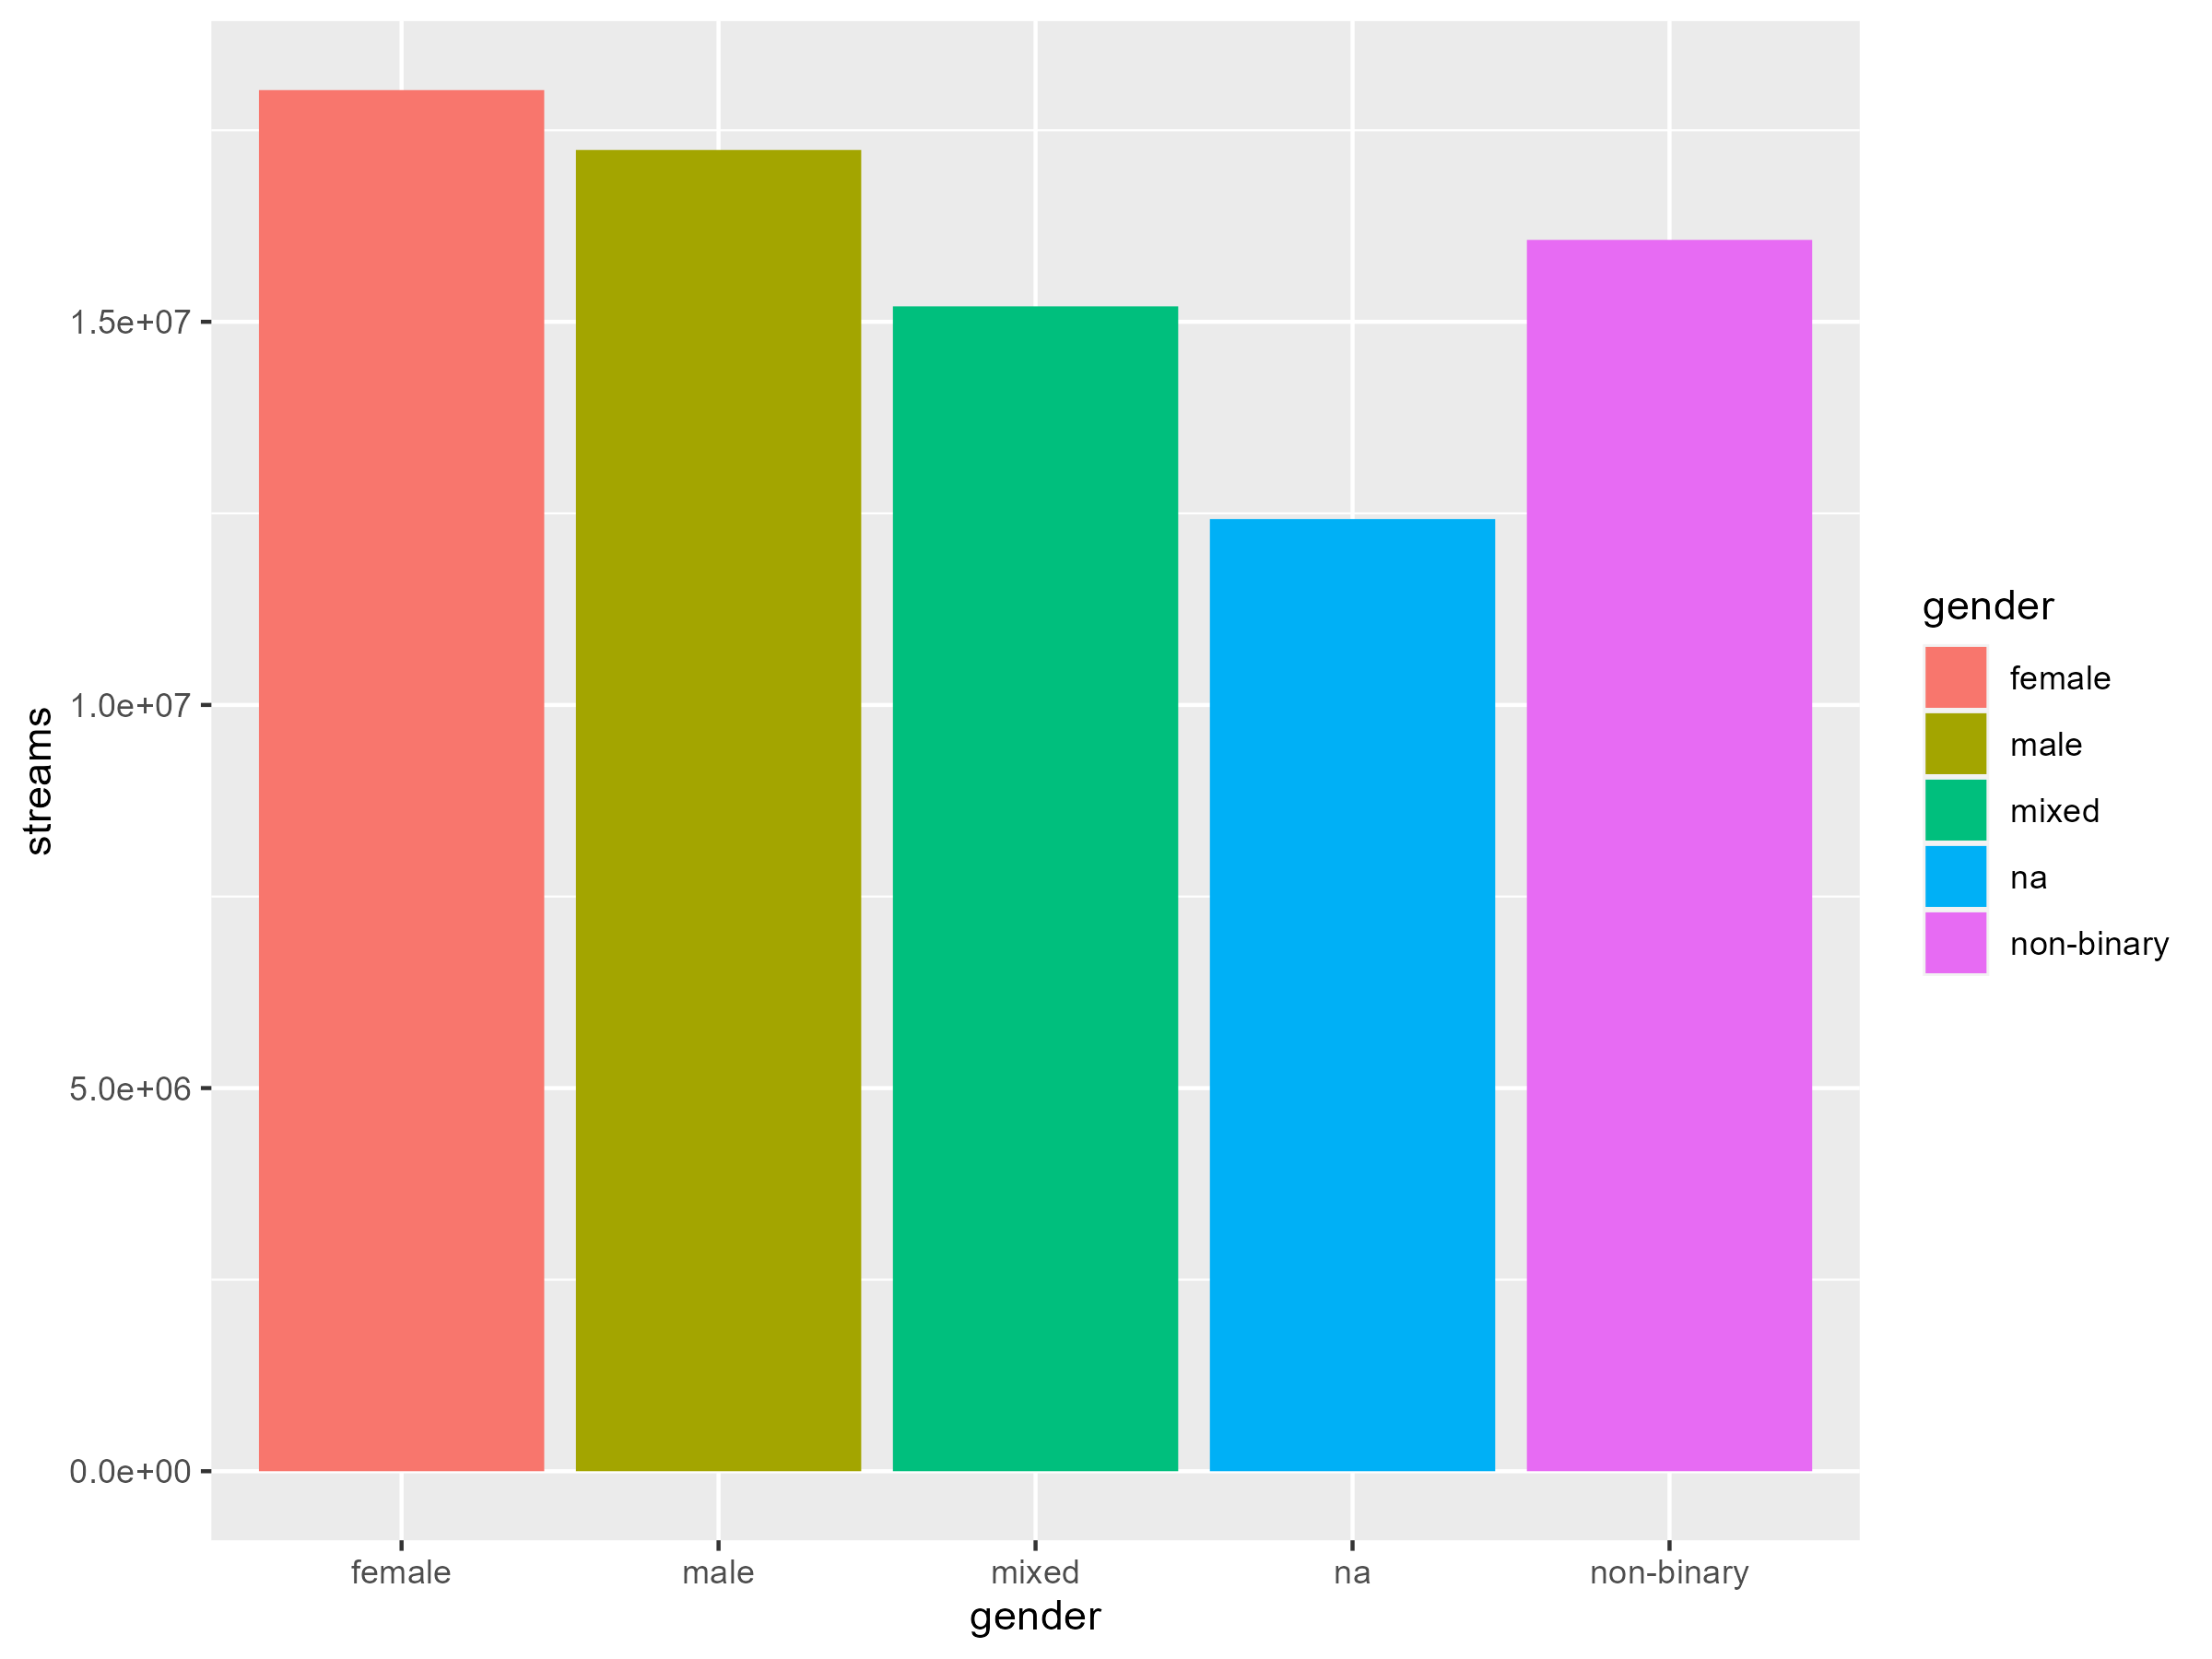
\includegraphics[width=0.95\linewidth]{Images/2_Bivariate/genderstreams.png}
        \caption{Bar plot \textit{gender} amb \textit{streams}}
        \label{fig:BivariateR_genderstreams}
    \end{minipage}%
    \begin{minipage}{.4\textwidth}
        \centering
        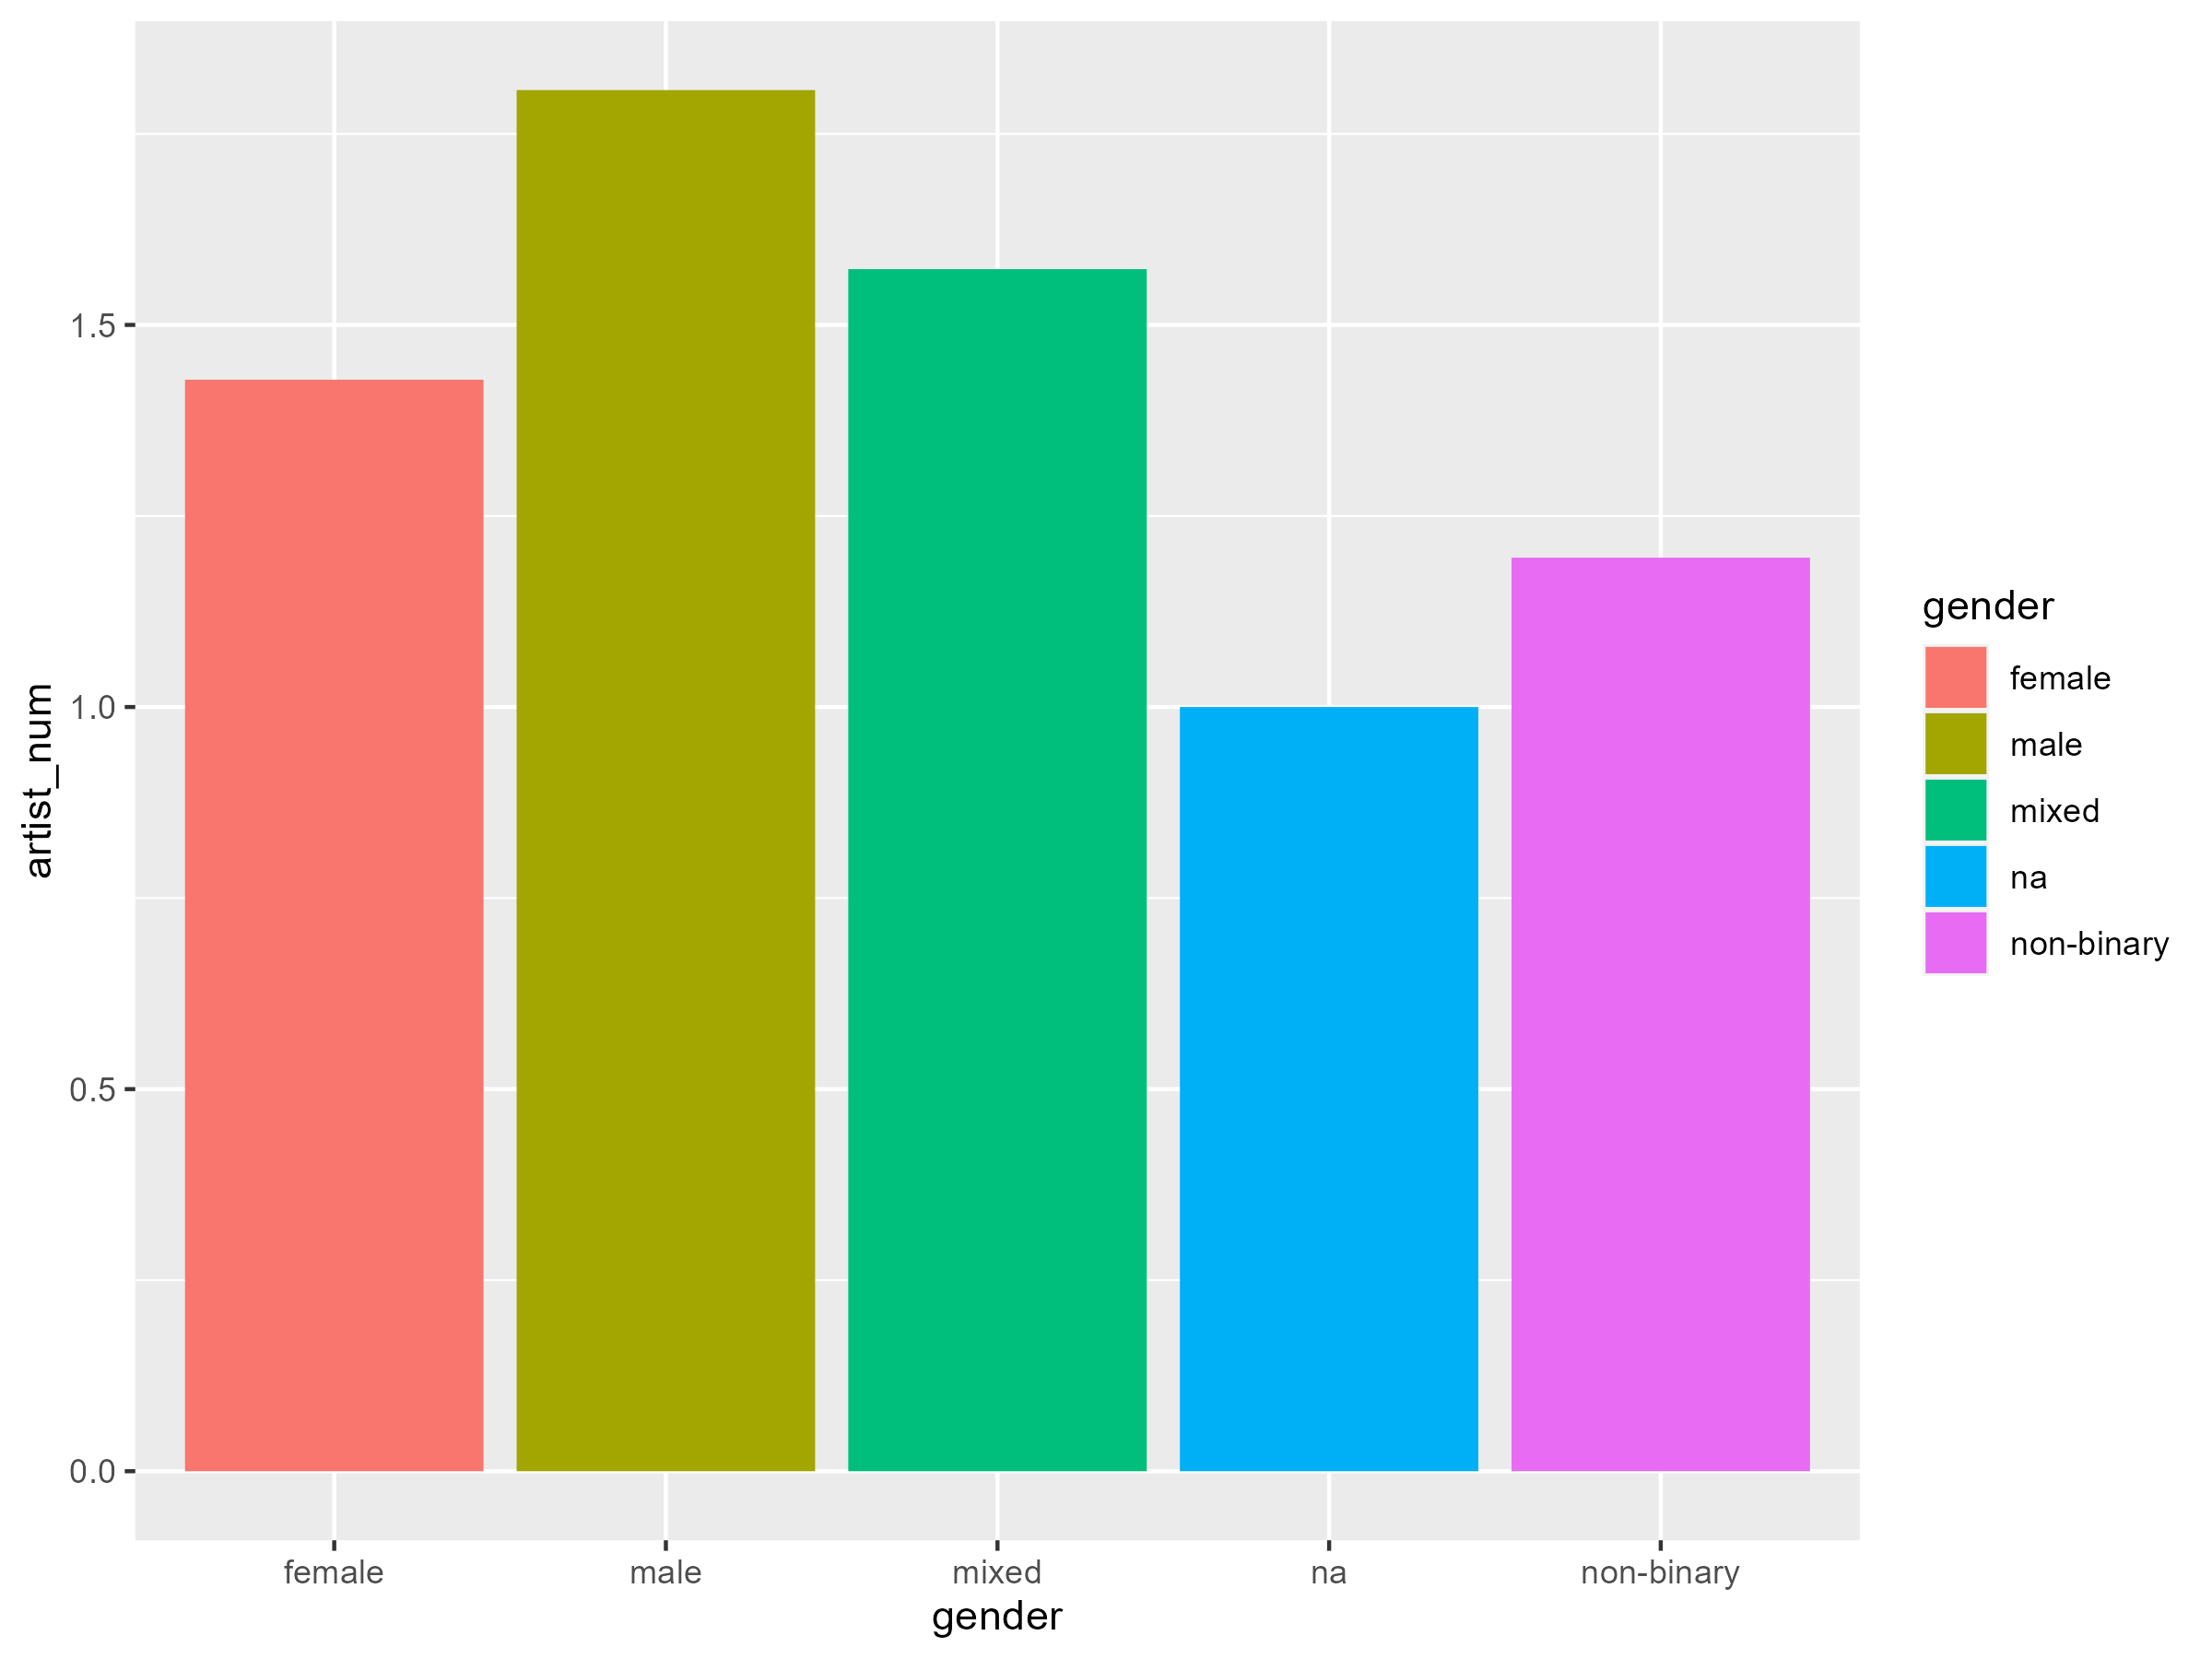
\includegraphics[width=0.95\linewidth]{Images/2_Bivariate/gendernum.png}
        \caption{Box plots \textit{gender} amb \textit{artist num}}
        \label{fig:BivariateR_gendernum}
    \end{minipage}%
\end{figure}

Analitzant la matriu de correlació (\ref{fig:BivariateR_correlation}), observem com hi ha bastanta correlació negativa entre acousticness i energy, fet que té sentit. Alhora, energy té correlació positiva amb loudness. Hi ha algunes variables que a penes tenen correlació amb cap altra, com és el cas de track\_popularity (excepte amb album popularity). Hi ha casos de variables que semblaria que podrien tenir una relació, com \textit{danceability} i \textit{energy}, però que resulta que no la tenen.

\begin{figure}[H]
    \centering
    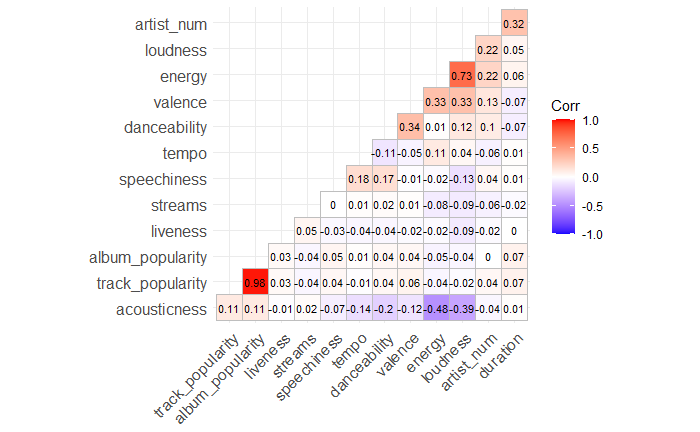
\includegraphics[width=0.8\textwidth]{Images/2_Bivariate/correlationvalues.png}
    \caption{Correlation matrix}
    \label{fig:BivariateR_correlation}
\end{figure}

Una alternativa de matriu de correlació és la figura \ref{fig:BivariateR_correlationdots} .Amb aquestes combinacions de variables numèriques, es pot veure usant scatter plots la correlació entre \textit{acousticness} i \textit{energy} (\ref{fig:BivariateR_acousticenergy}), \textit{energy} i \textit{loudness} (\ref{fig:BivariateR_energyloud}) o bé la poca entre \textit{danceability} i \textit{valence} (\ref{fig:BivariateR_danceval}).

\begin{figure}[H]
\centering
    \begin{minipage}{.4\textwidth}
        \centering
        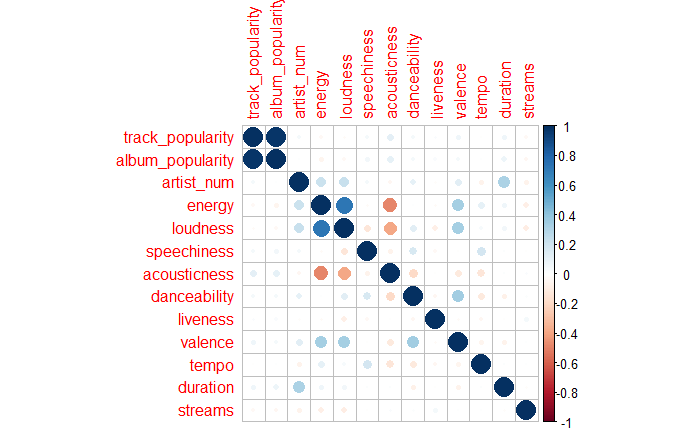
\includegraphics[width=0.95\linewidth]{Images/2_Bivariate/correlationdots.png}
        \caption{Matriu de correlació alternativa}
        \label{fig:BivariateR_correlationdots}
    \end{minipage}%
    \begin{minipage}{.4\textwidth}
        \centering
        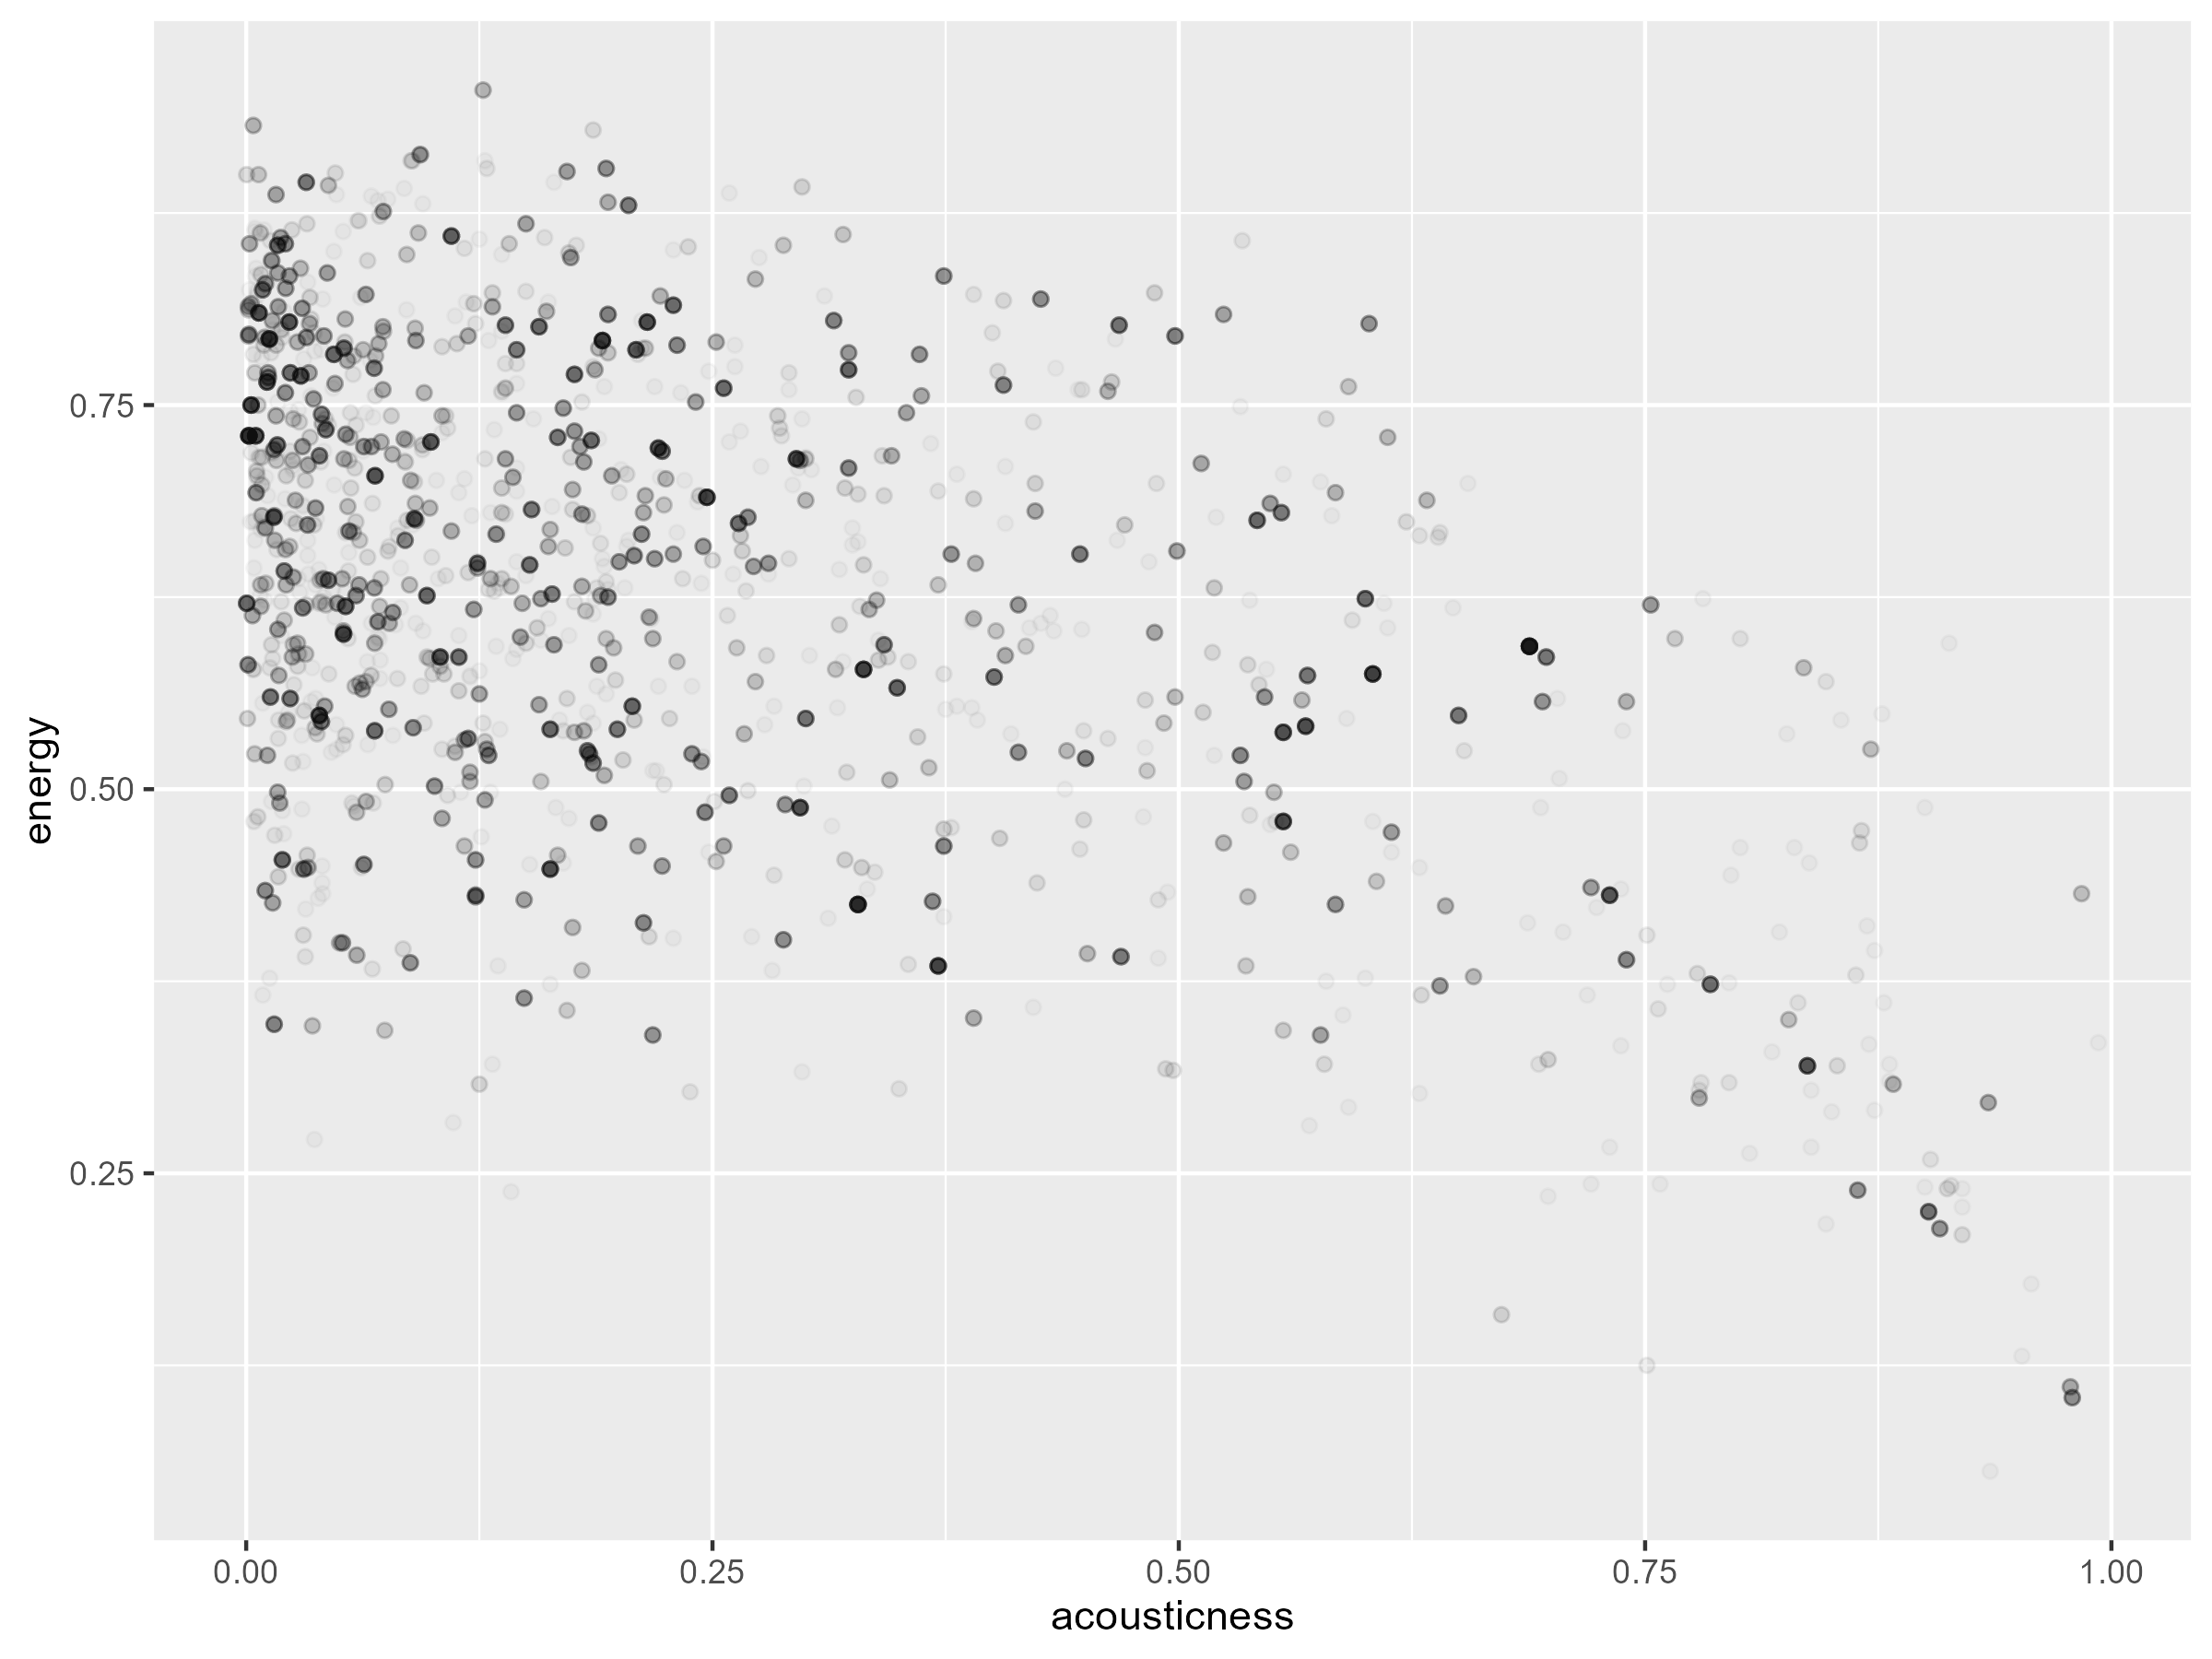
\includegraphics[width=0.95\linewidth]{Images/2_Bivariate/acousticenergy.png}
        \caption{Scatter plot de \textit{acousticness} amb \textit{energy}}
        \label{fig:BivariateR_acousticenergy}
    \end{minipage}%
\end{figure}
\begin{figure}[H]
\centering
    \begin{minipage}{.4\textwidth}
        \centering
        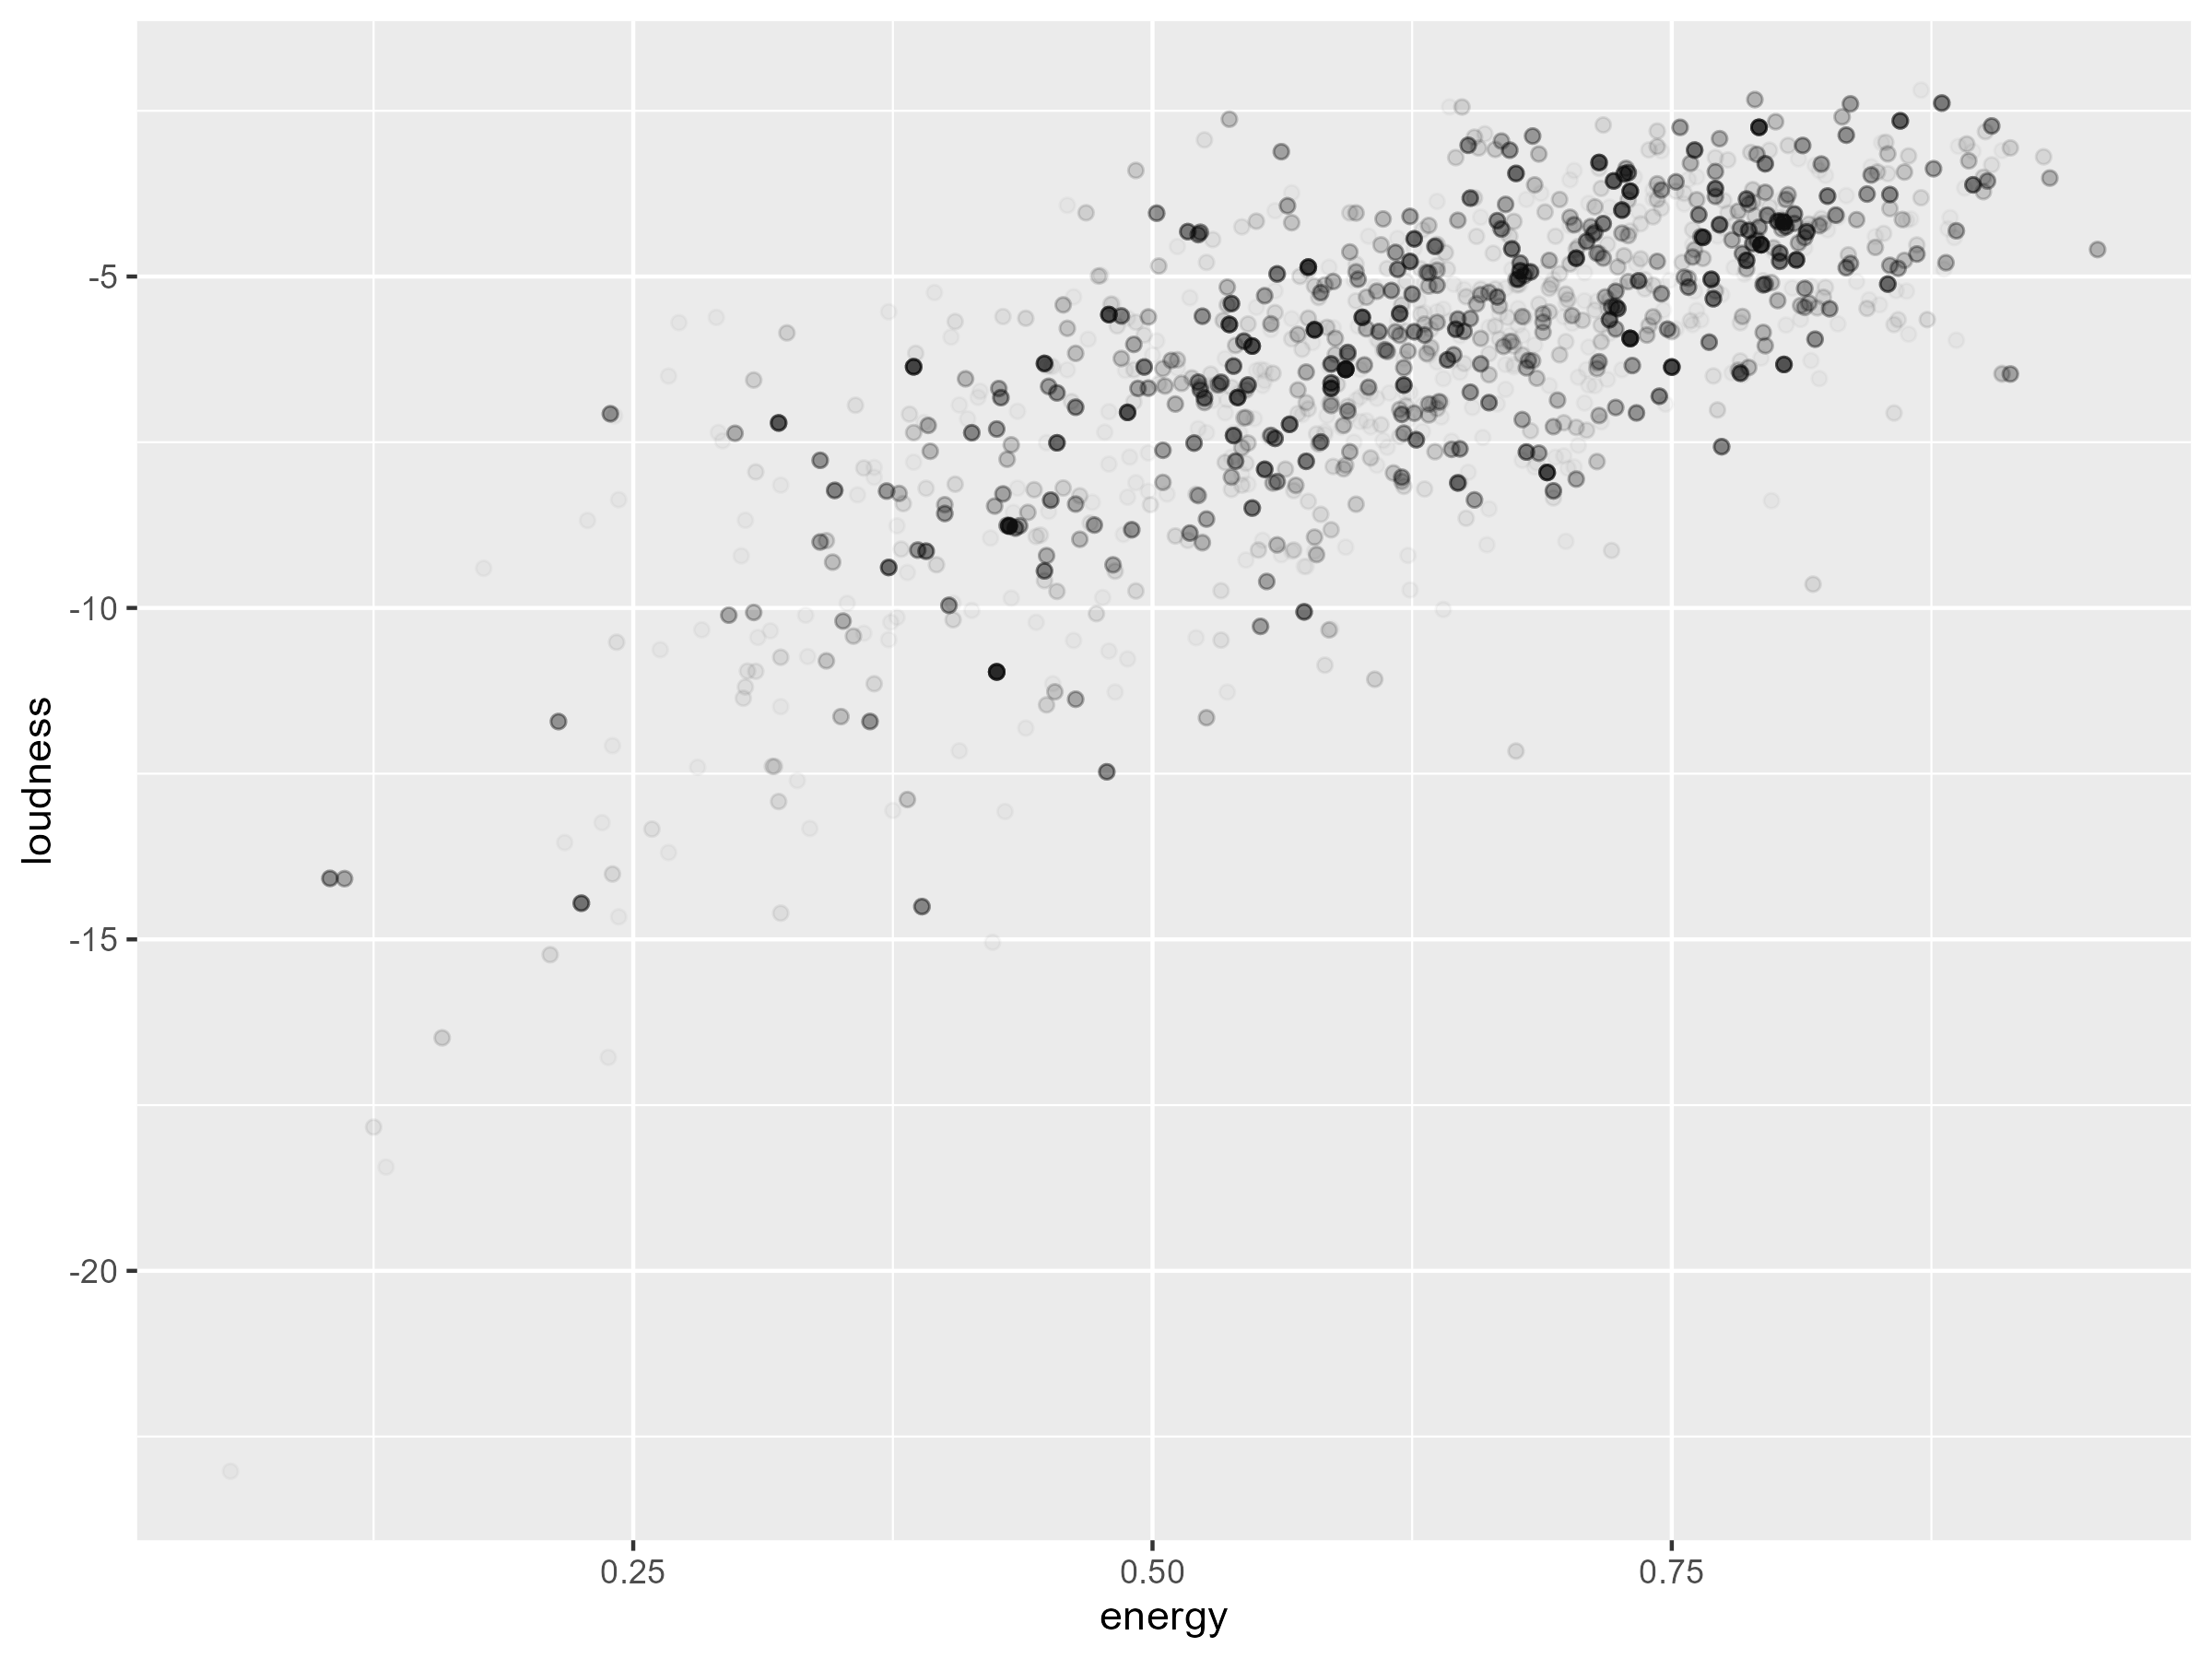
\includegraphics[width=0.95\linewidth]{Images/2_Bivariate/energyloudness.png}
        \caption{Scatter plot de \textit{energy} amb \textit{loudness}}
        \label{fig:BivariateR_energyloud}
    \end{minipage}%
    \begin{minipage}{.4\textwidth}
        \centering
        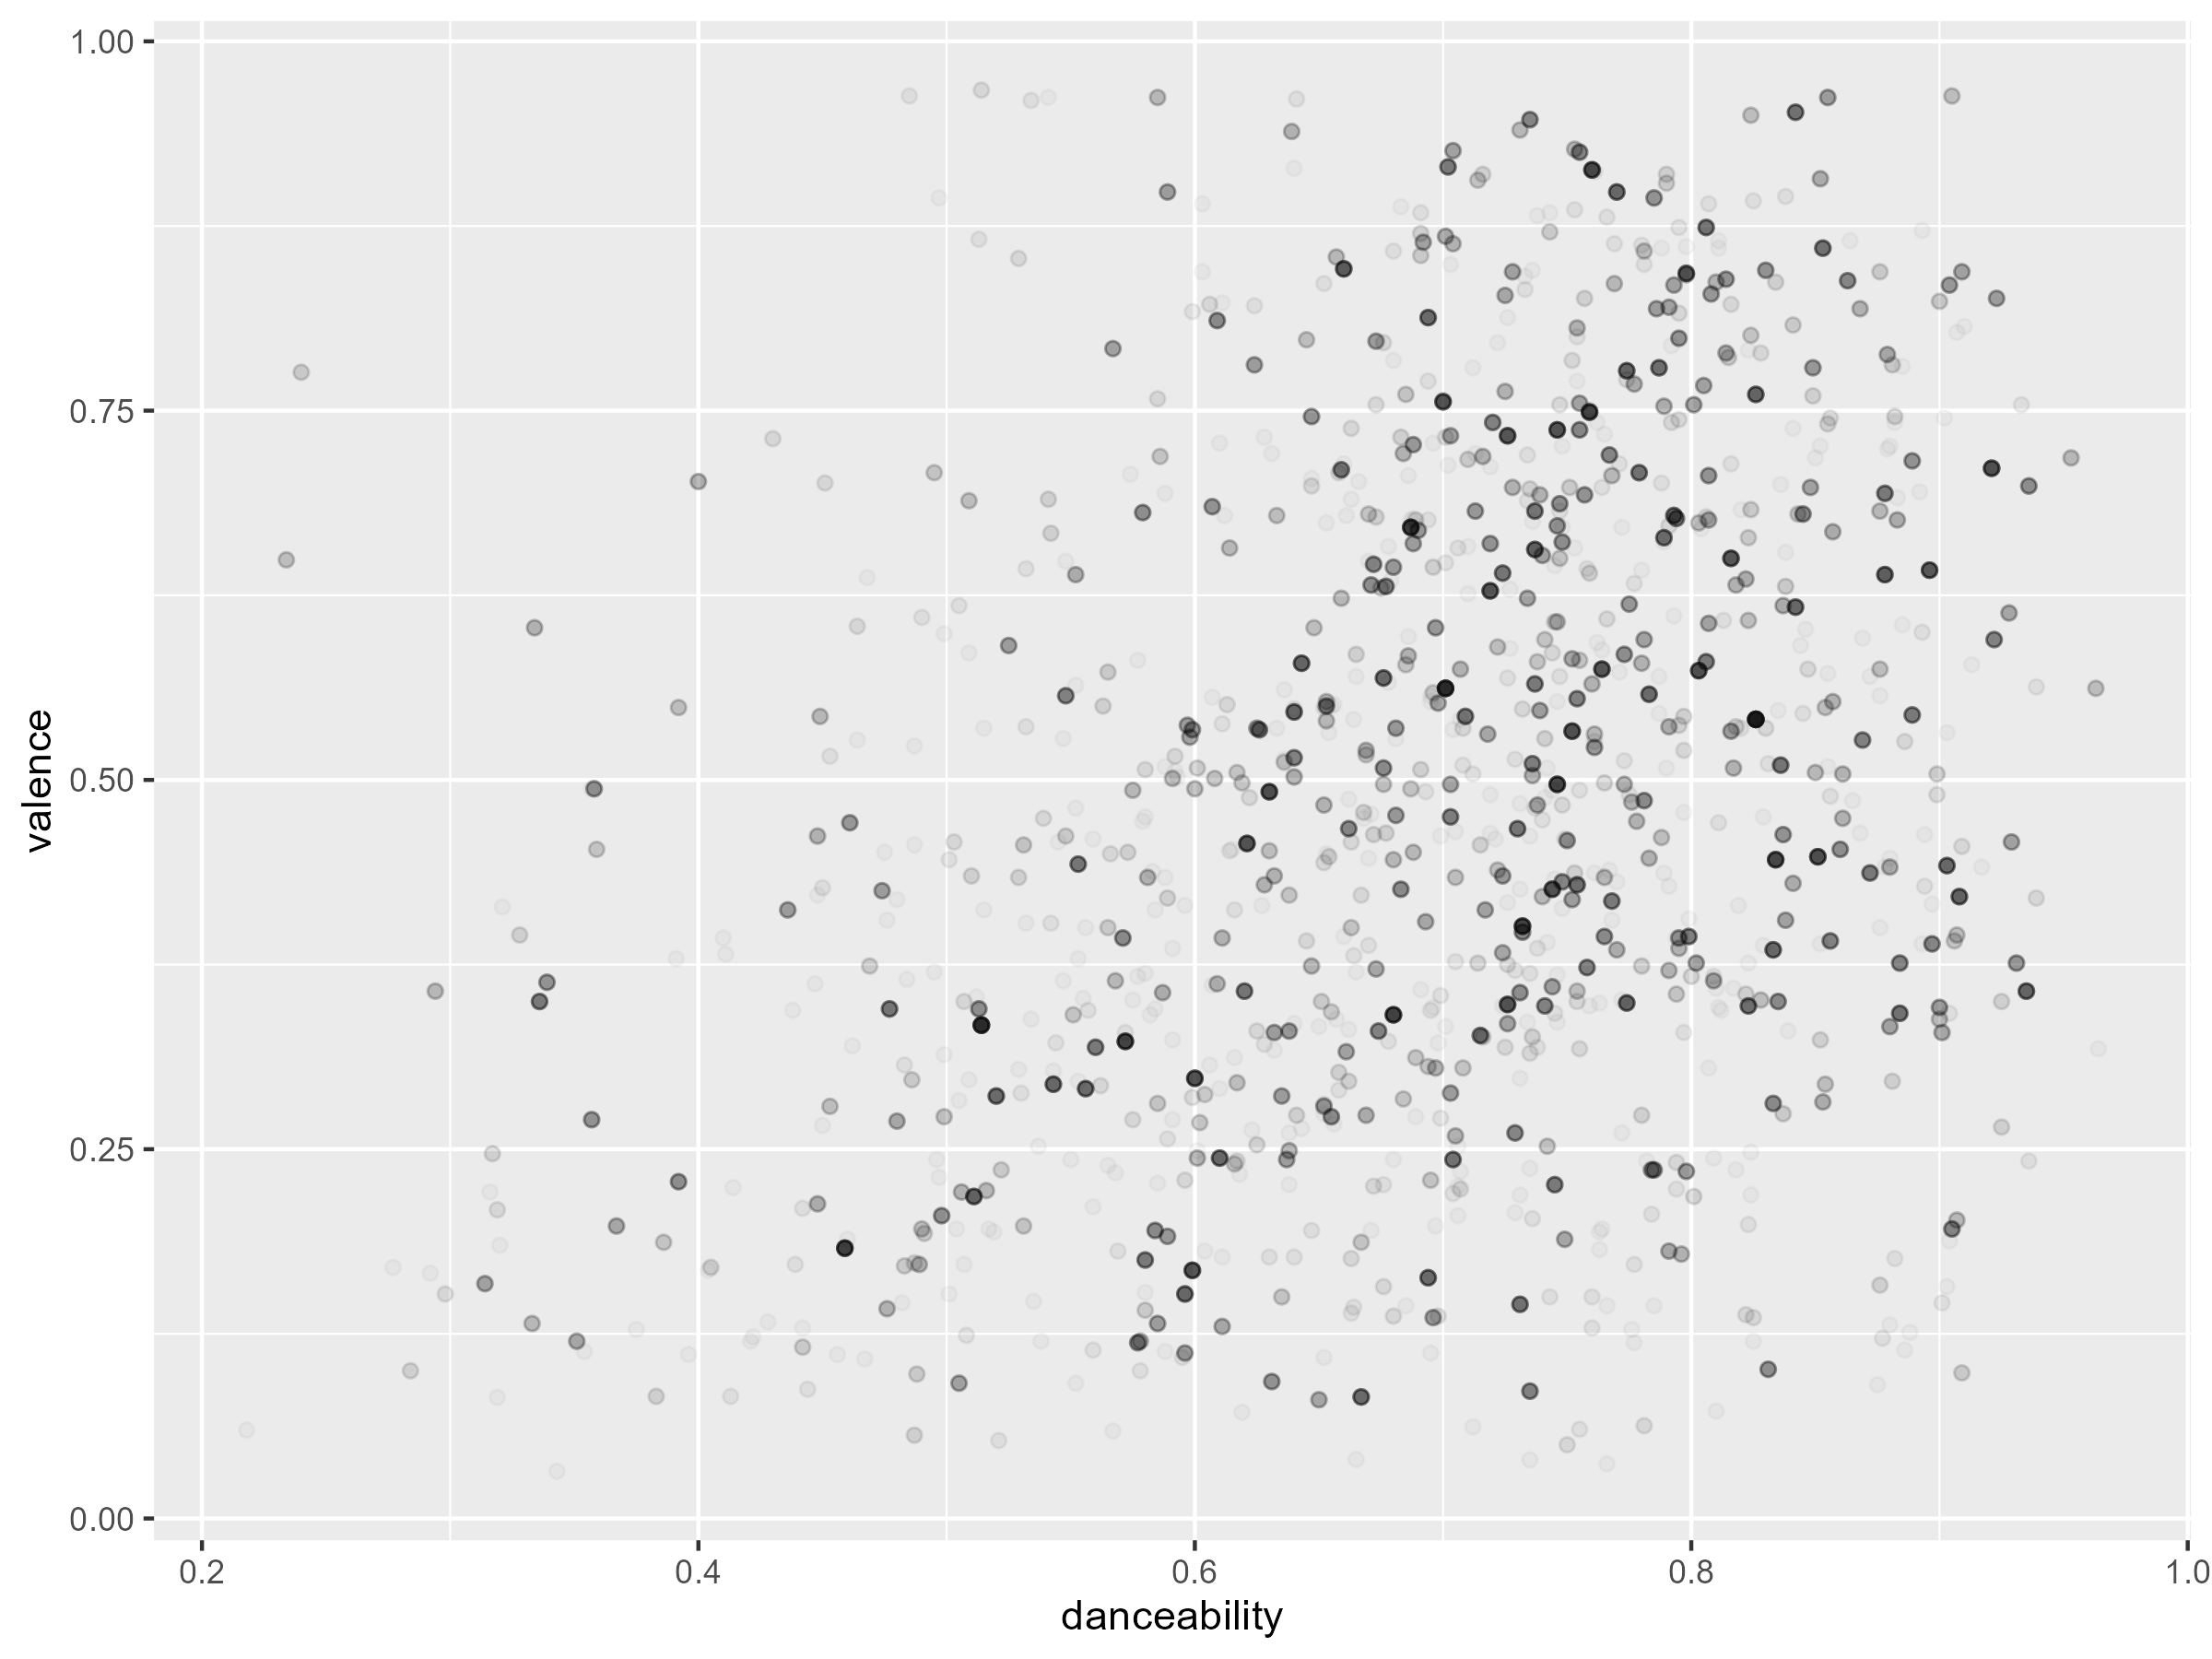
\includegraphics[width=0.95\linewidth]{Images/2_Bivariate/danceabilityvalence.png}
        \caption{Scatter plot de \textit{danceability} amb \textit{valence}}
        \label{fig:BivariateR_danceval}
    \end{minipage}%
\end{figure}

Finalment, pel que fa a les parelles de variables categòriques, es pot observar que hi ha molt poques cançons que siguin electro i no pop (per tant, la majoria de cançons electro serien electropop) (\ref{fig:BivariateR_electropop}). La majoria d'artistes del gènere femení realitzen cançons de pop (\ref{fig:BivariateR_popgender}), mentre que el hip hop el dominen els homes (\ref{fig:BivariateR_hiphopgender}). Hi ha poques cançons explícites que no siguin de hip hop, tan sols apareixen 5 cançons d'electro i latino, i no hi ha grups de latino (\ref{fig:BivariateR_latinogroup}).

\begin{figure}[H]
\centering
    \begin{minipage}{.4\textwidth}
        \centering
        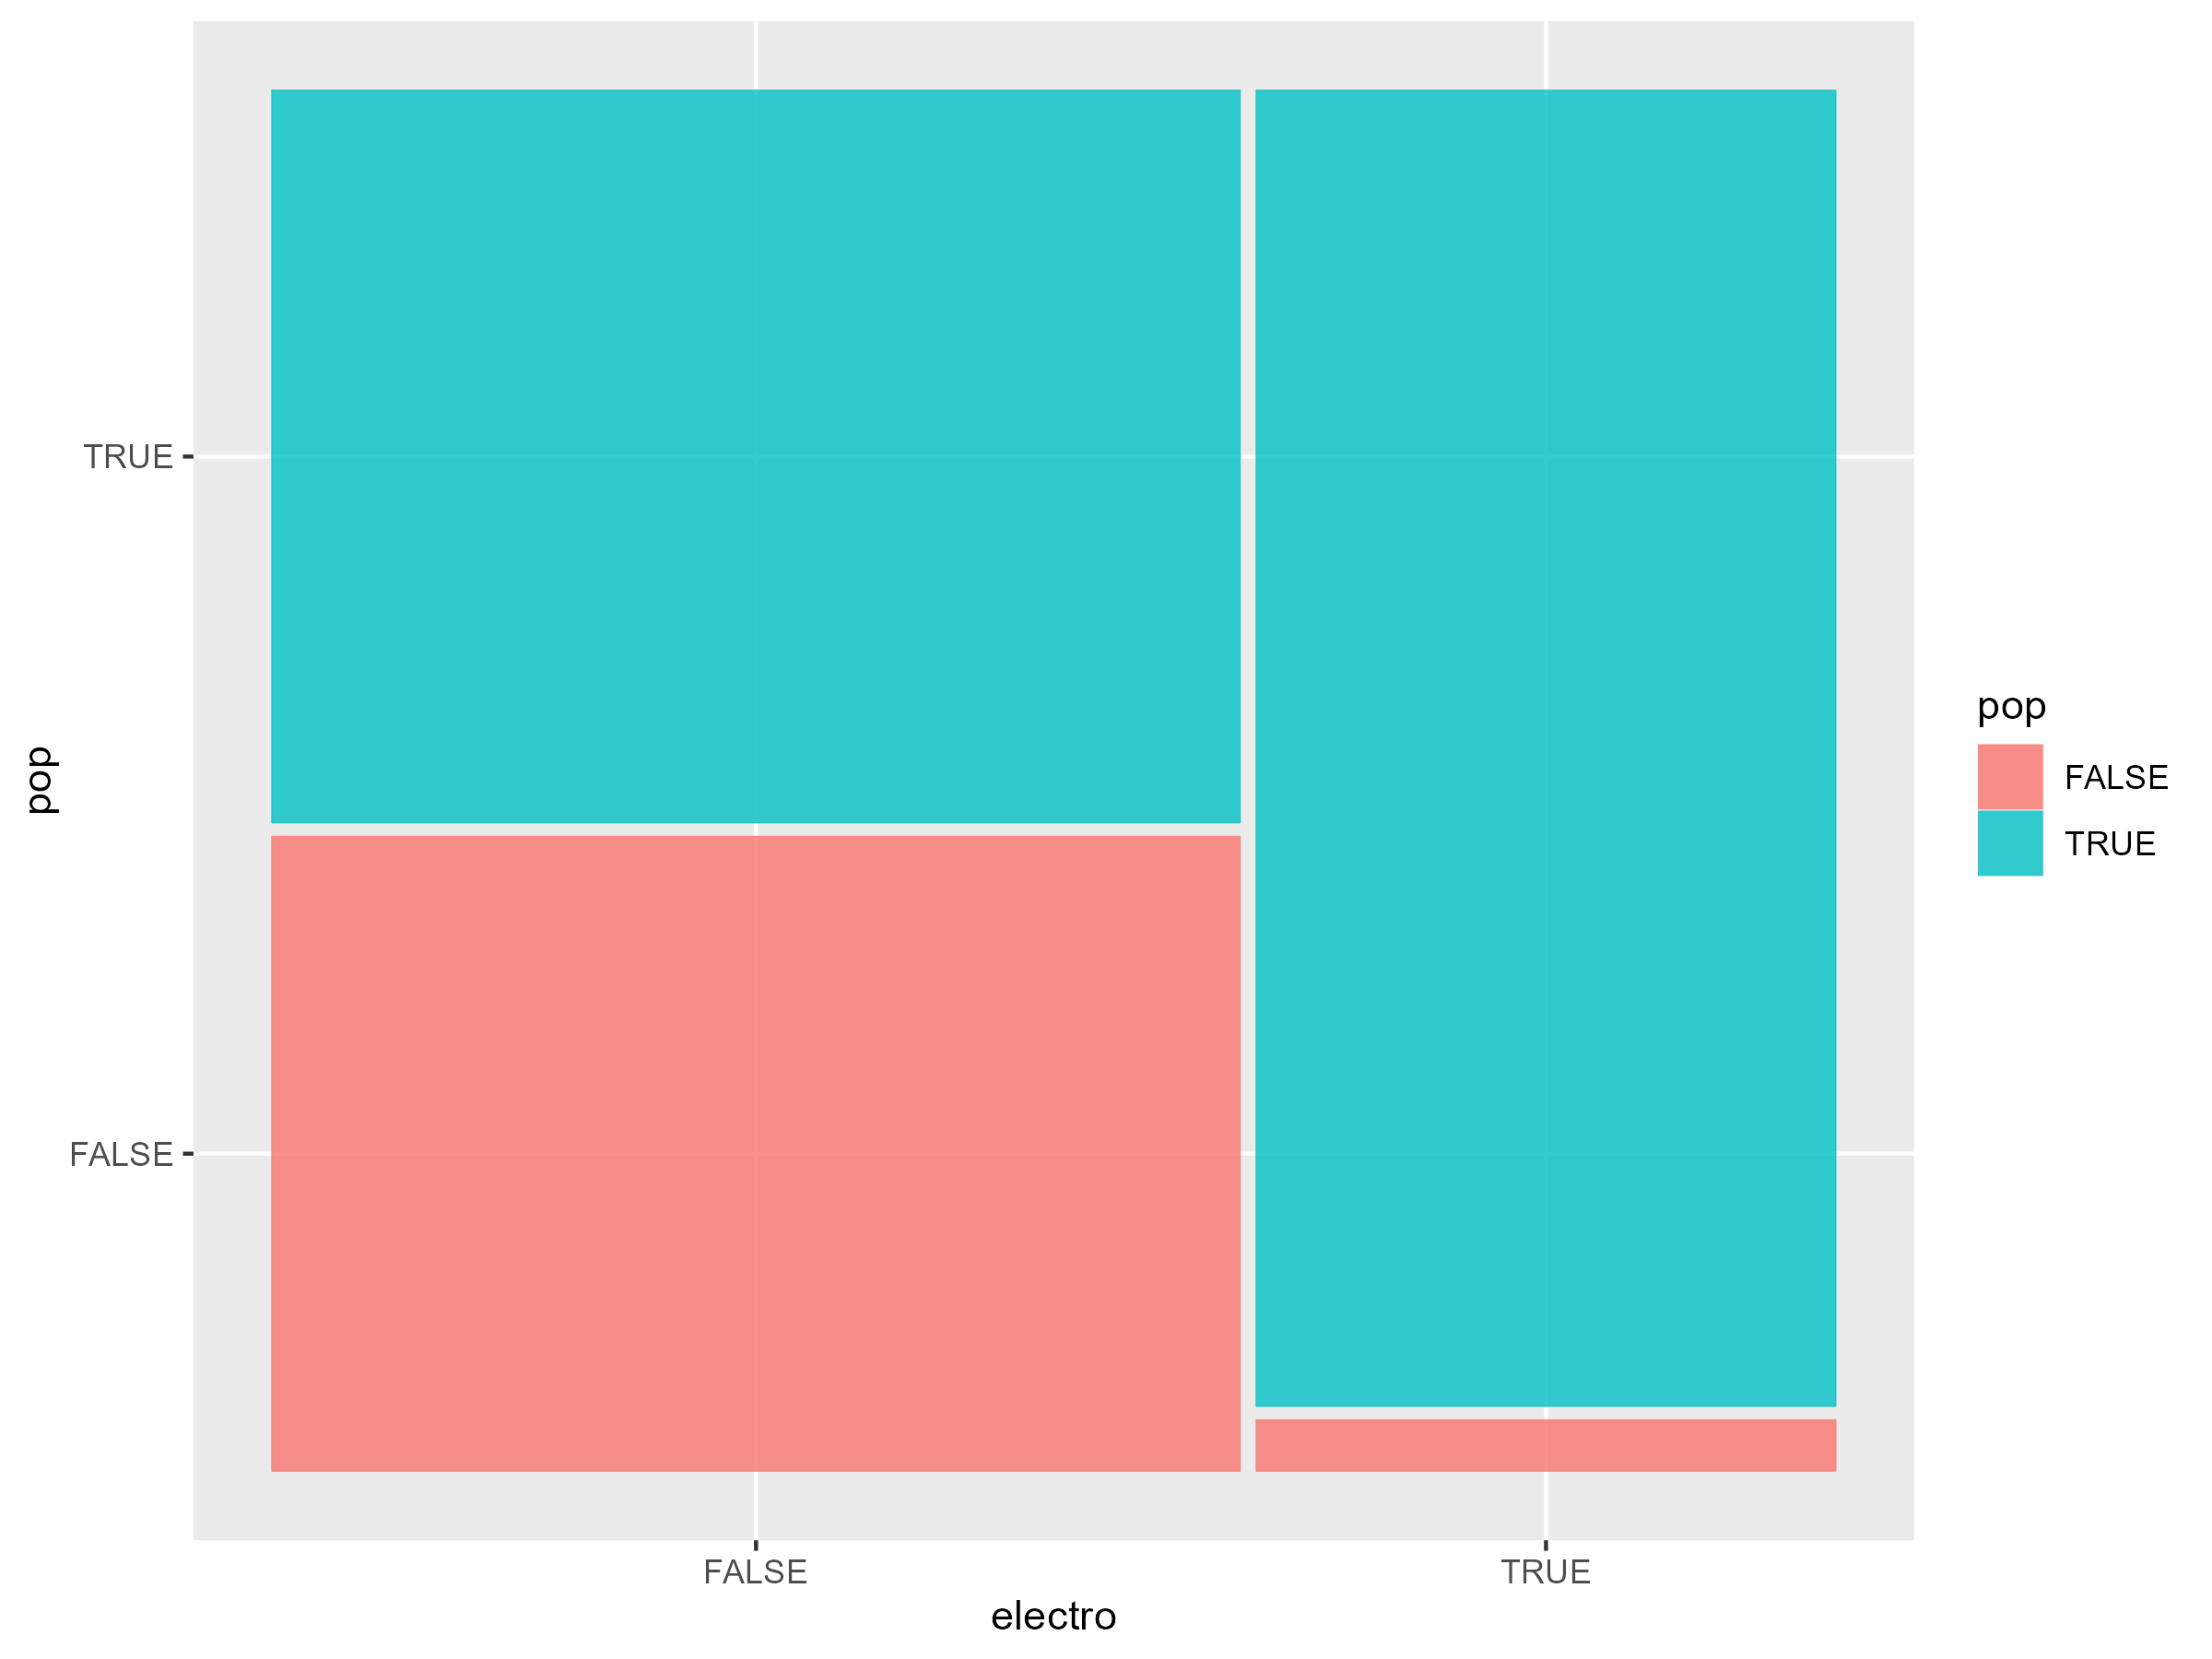
\includegraphics[width=0.95\linewidth]{Images/2_Bivariate/electropop.png}
        \caption{Bar plots \textit{electro} amb \textit{pop}}
        \label{fig:BivariateR_electropop}
    \end{minipage}%
    \begin{minipage}{.4\textwidth}
        \centering
        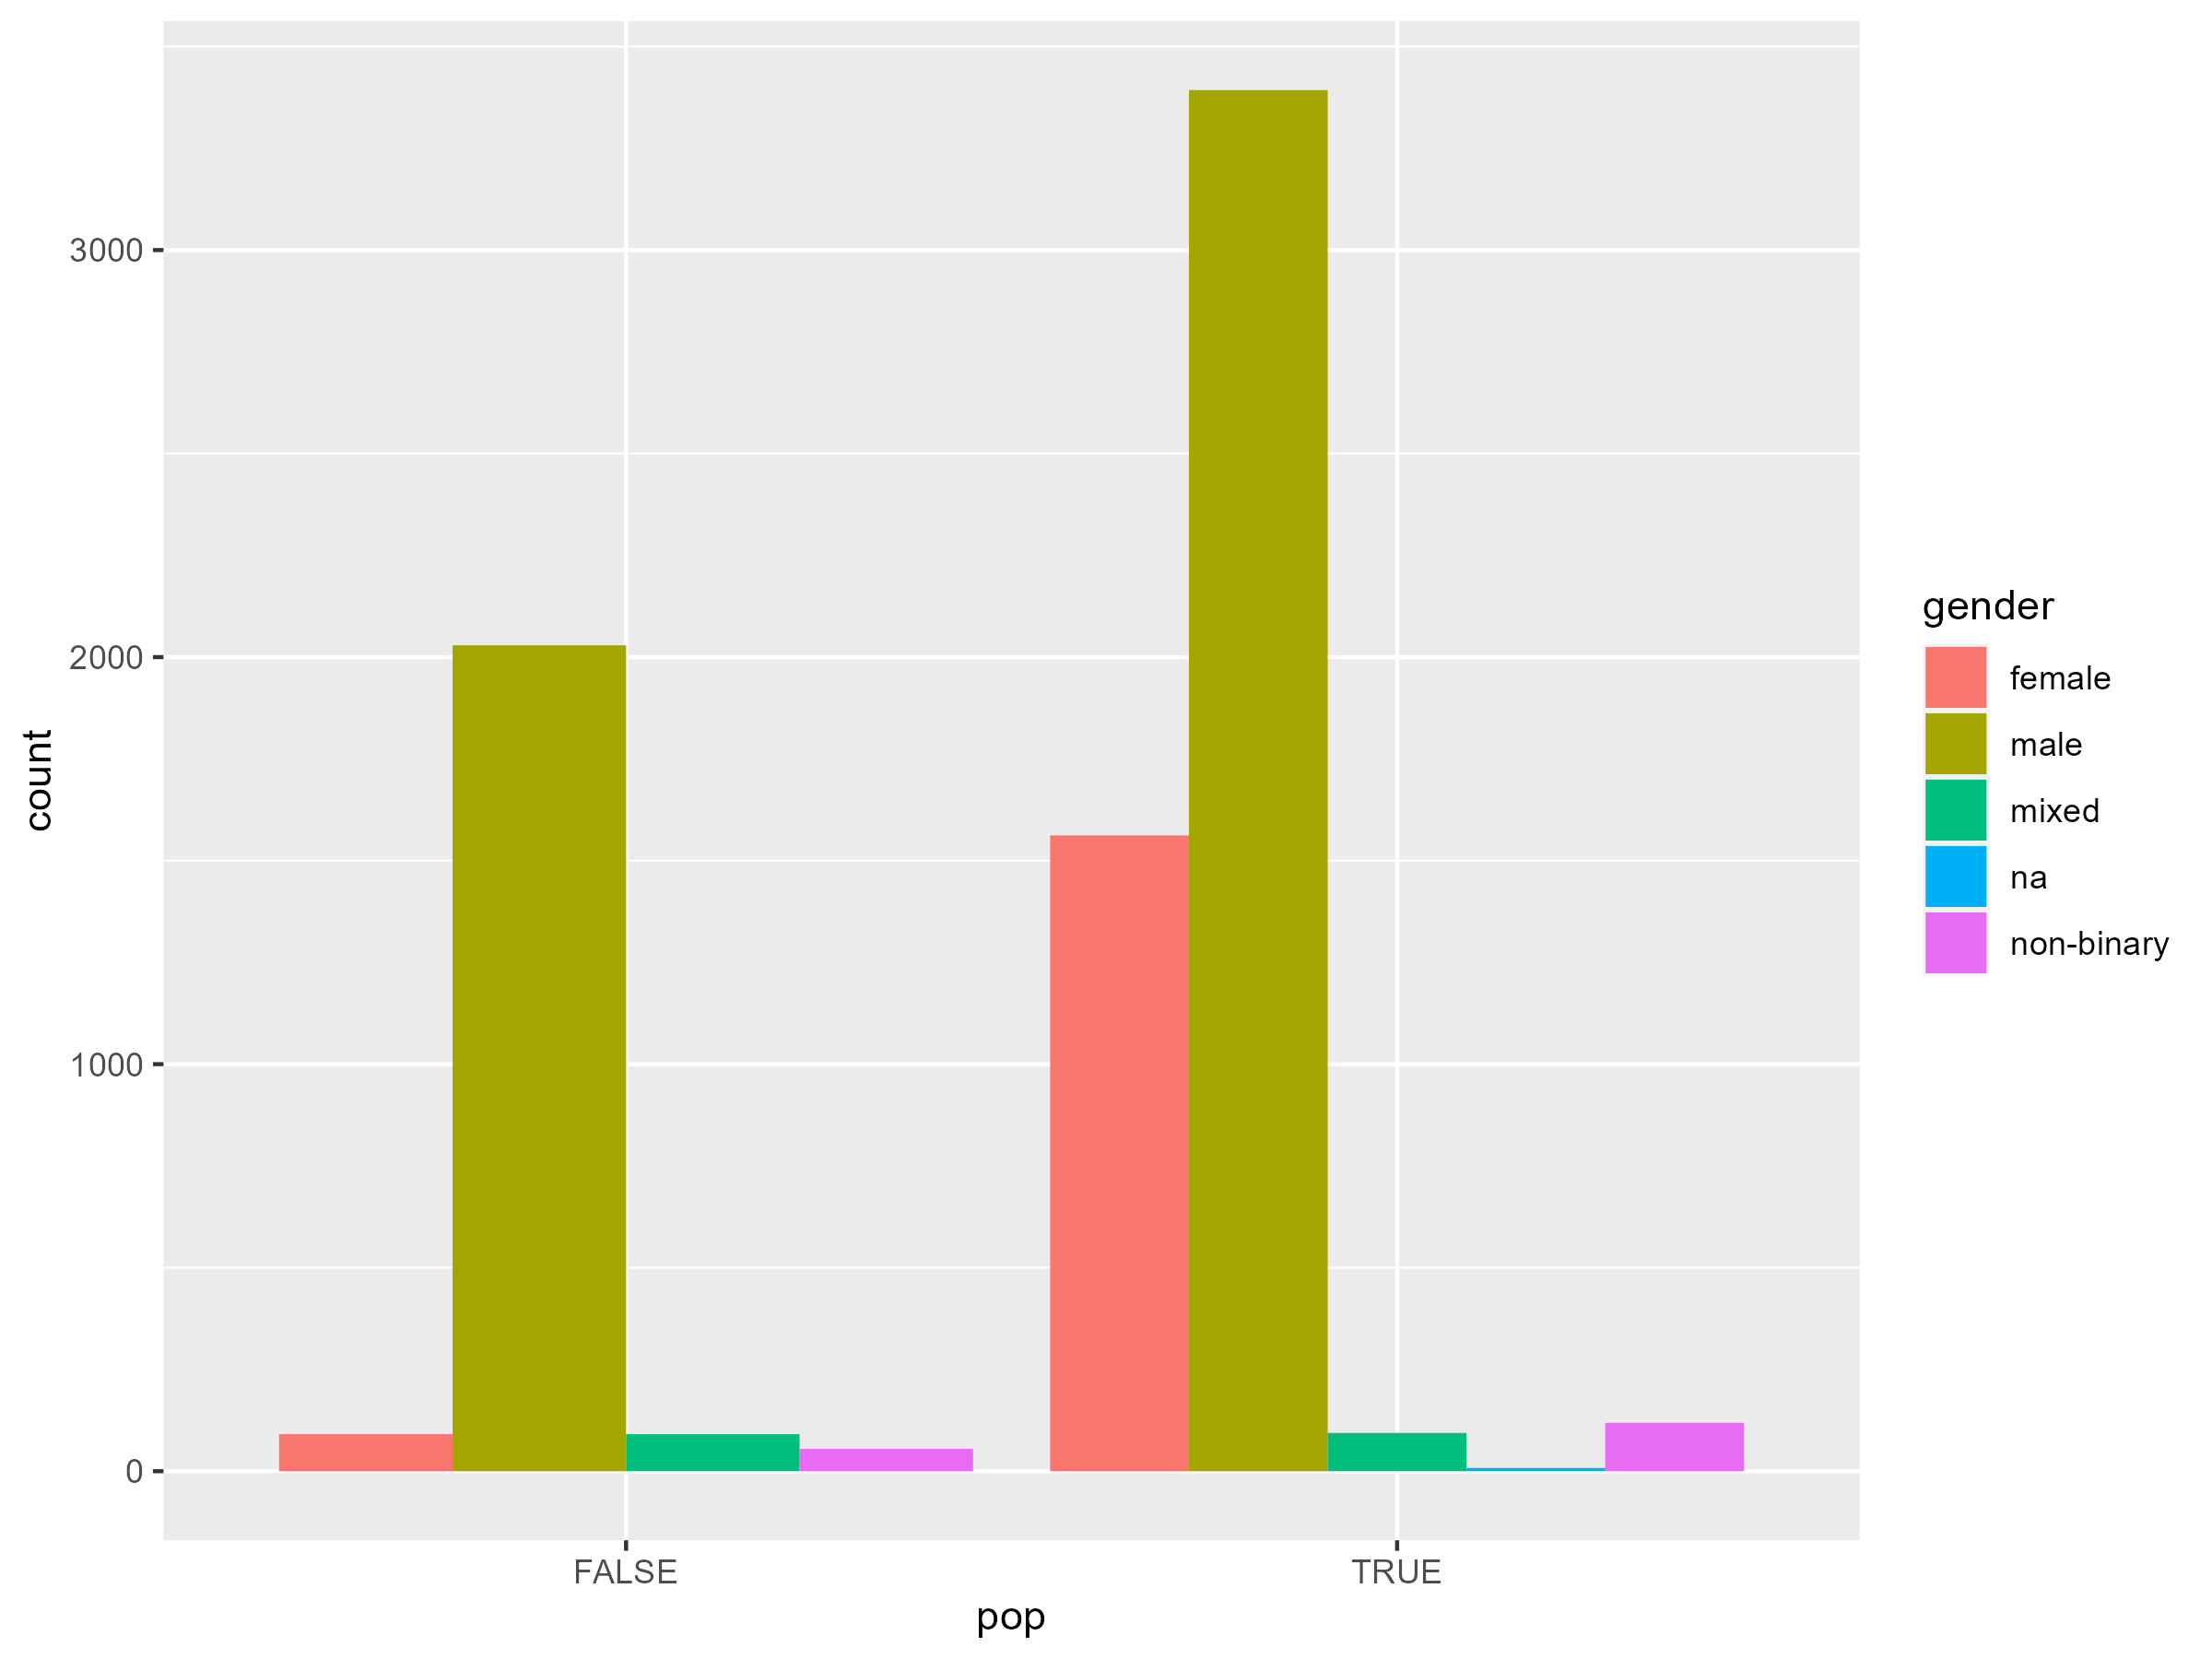
\includegraphics[width=0.95\linewidth]{Images/2_Bivariate/popgender.png}
        \caption{Bar plots \textit{gender} amb \textit{pop}}
        \label{fig:BivariateR_popgender}
    \end{minipage}%
\end{figure}
\begin{figure}[H]
\centering
    \begin{minipage}{.4\textwidth}
        \centering
        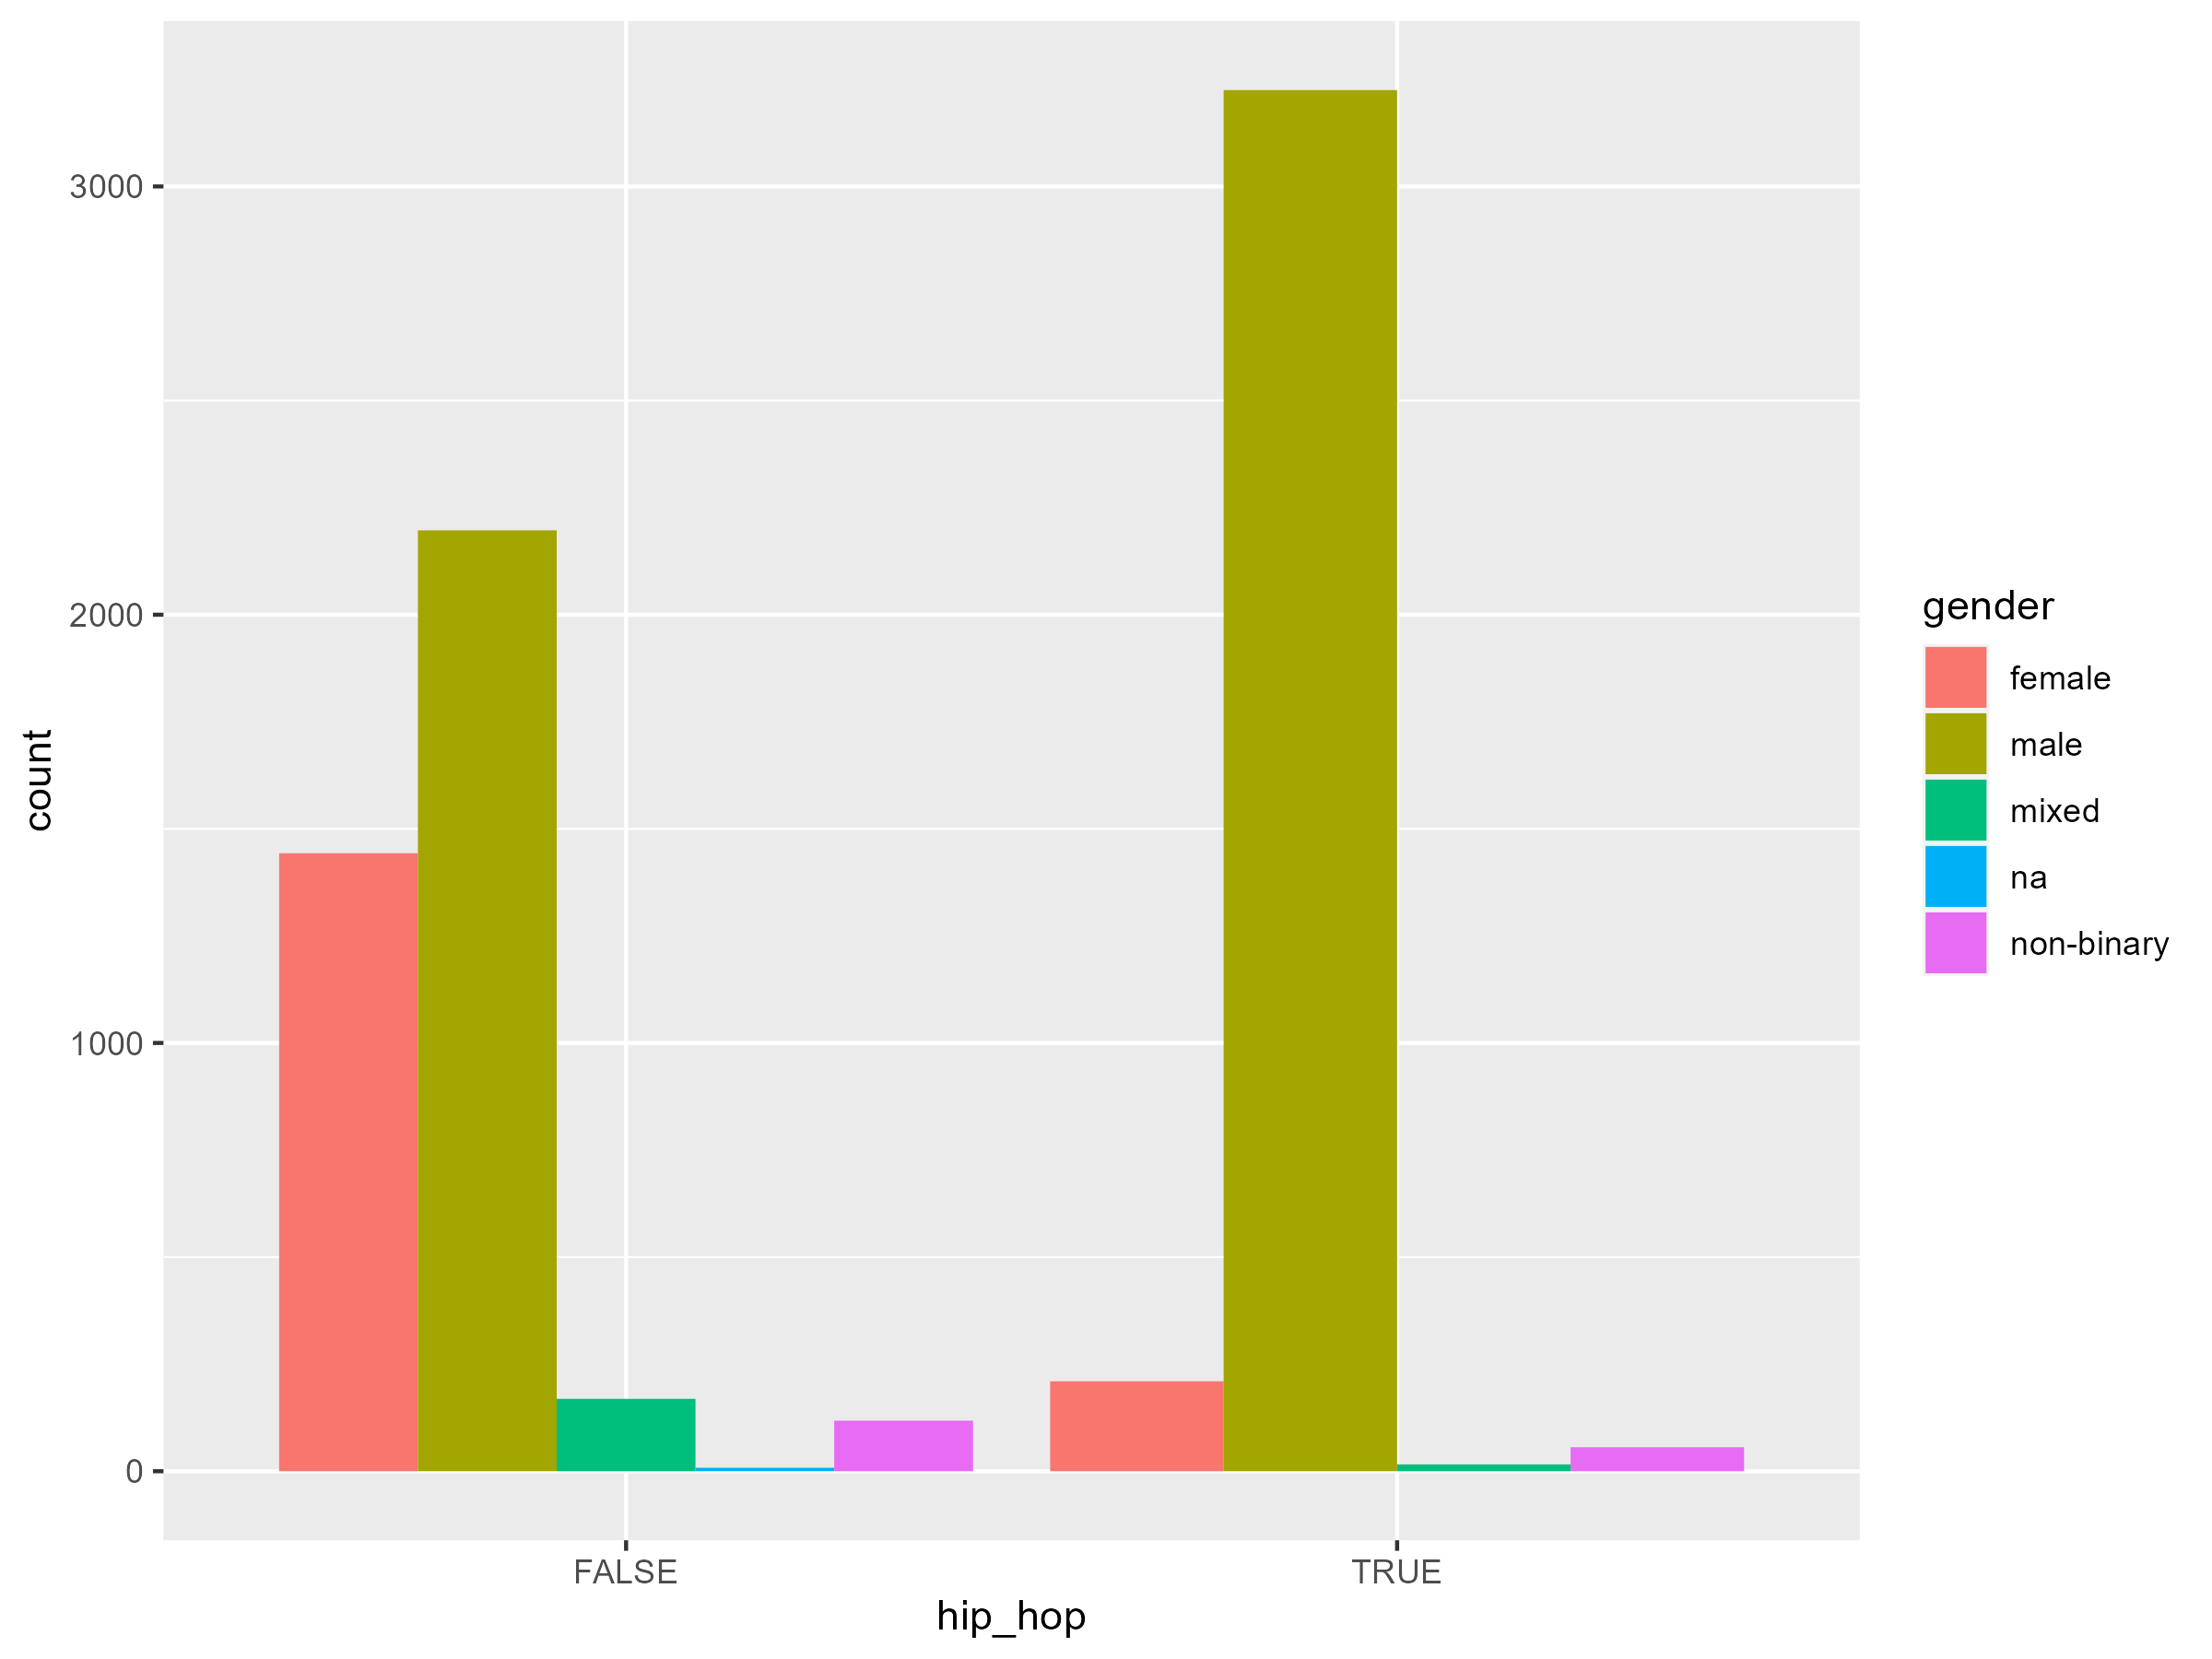
\includegraphics[width=0.95\linewidth]{Images/2_Bivariate/hiphopgender.png}
        \caption{Bar plost \textit{gender} amb \textit{hip hop}}
        \label{fig:BivariateR_hiphopgender}
    \end{minipage}%
    \begin{minipage}{.4\textwidth}
        \centering
        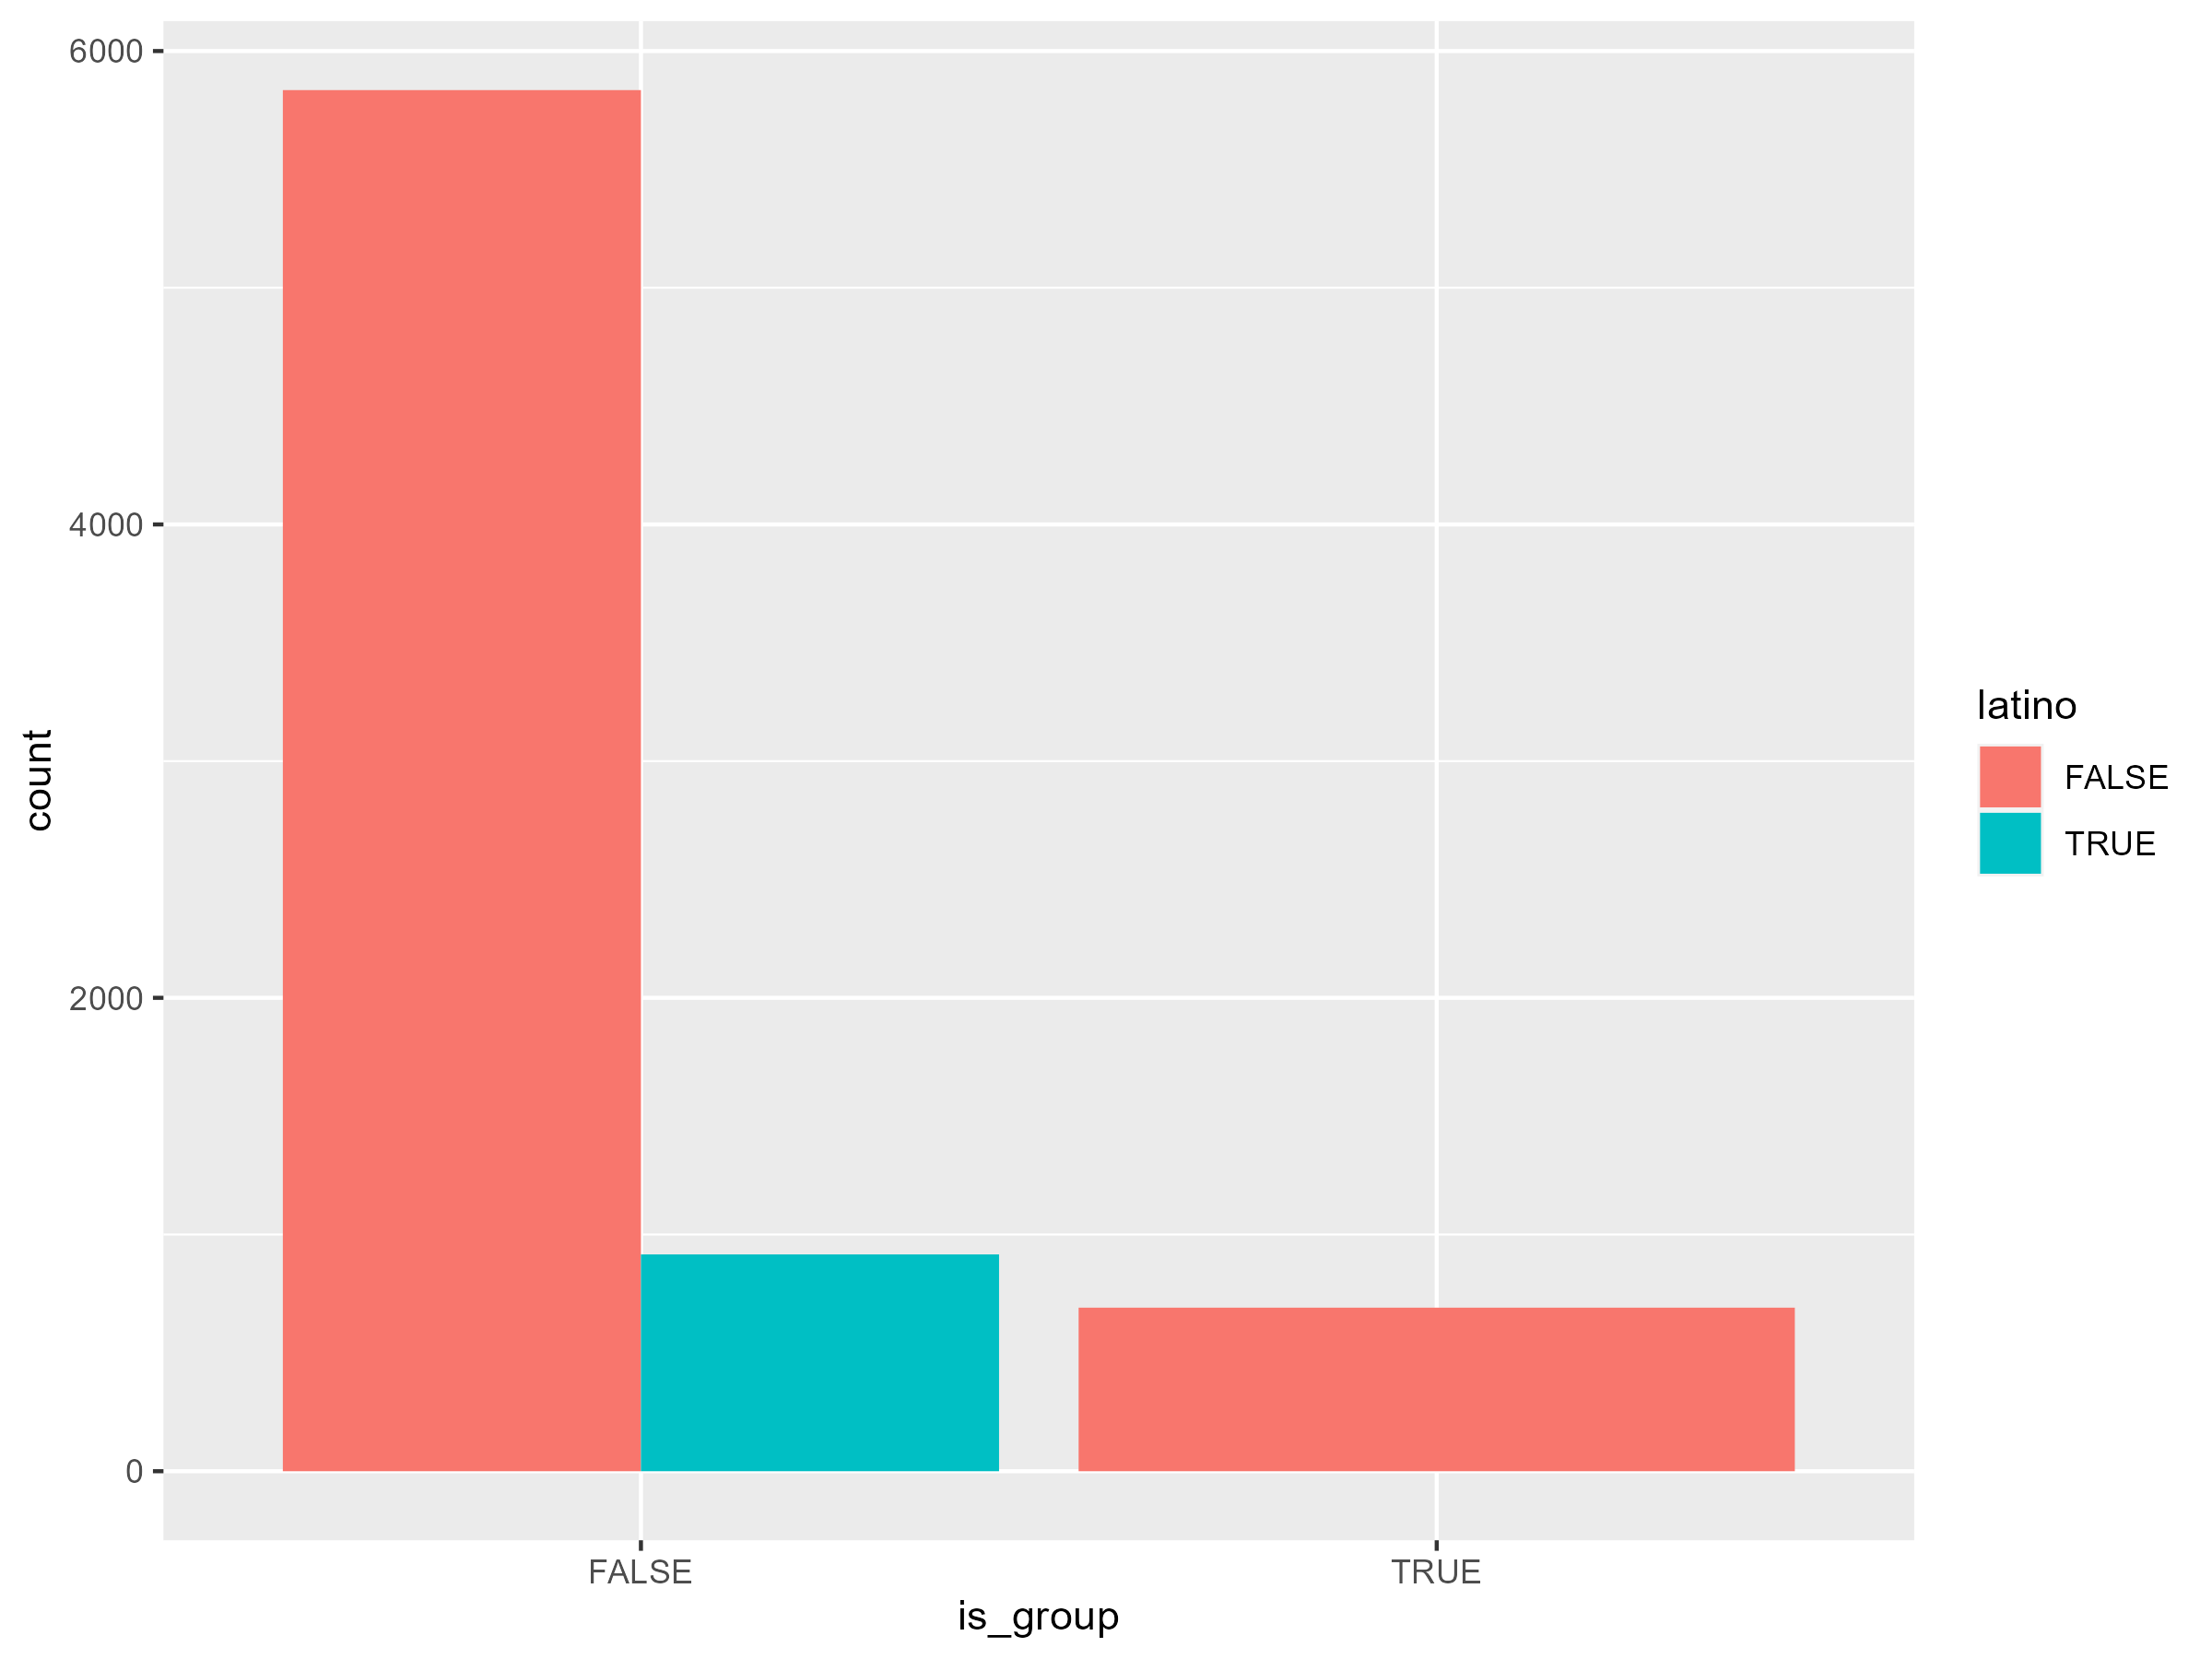
\includegraphics[width=0.95\linewidth]{Images/2_Bivariate/latinogroup.png}
        \caption{Box plots \textit{latino} amb \textit{is group}}
        \label{fig:BivariateR_latinogroup}
    \end{minipage}%
\end{figure}

En conclusió, amb aquest anàlisi bivariant no hem observat realment cap comportament estrany. En alguns casos, es podria arribar a considerar algun punt com a outlier bivariant, però aquest fet es deu més a que tenim dades bastant esparses. A més, hem observat que la majoria de les variables numèriques a penes tenen correlació entre elles, i les categòriques tampoc en tenen molta.

És important comentar que no s’han tractat outliers, encara que n’hi hagi (especialment en variables com artist followers o streams). L’argumentació per no eliminar-los, convertir-los en dades mancants i imputar-los o tractar-los d’alguna altra forma és principalment que es tracten de dades reals. No es pot no tenir en compte un artista que tot i tenir pocs seguidors hagi estat capaç de crear un hit, per exemple, ja que és un cas que va ocòrrer així en la realitat. Aquestes dades provenen de la API de Spotify directament, que està ben treballada i en principi no hauria de contenir dades errònies (ni se n’han detectat en aquest EDA inicial) i per tant no considerarem cap valor com a extrany.

Aquest anàlisi univariant i bivariant han permés definir quins eren els passos a dur a terme durant el preprocessament, que es comentaran a continuació.
